\input{glyphtounicode}\pdfgentounicode=1 % searchable, copyable text (pdflatex)
% ECCE by Example: worked calculations that show what ECCE does.
% Build: make   (lualatex, makeindex, bibtex; see README.md)
\documentclass[
	11pt,
	fleqn,
	a4paper,
]{LegrandOrangeBook}
% No font expansion: stretched glyphs make single words look like another font.
\microtypesetup{expansion=false}

\usepackage[english]{babel}
\usepackage{amsmath}
\usepackage{amssymb}
\usepackage{graphicx}
\usepackage{placeins}
\usepackage{float}
\usepackage[version=4]{mhchem}
\usepackage{siunitx}
\usepackage{makeidx}
\makeindex

\setcounter{tocdepth}{2}
\graphicspath{{figures/}}

% Conventions used throughout the book.
\newcommand{\ecceversion}{9.5.2}
% Menu paths and controls: \menu{Tools > Diffraction...}, \ctrl{Calculate}
\newcommand{\menu}[1]{\textbf{\sffamily #1}}
\newcommand{\ctrl}[1]{\textbf{\sffamily #1}}
% Commands and file names
\newcommand{\cmd}[1]{\texttt{#1}}
% The example set holding a chapter's finished calculation, when there is one (optional)
\newcommand{\eccexample}[1]{\par\noindent\textit{Example set:} \menu{#1}\par}
% Placeholder for a fact still to be checked (voice guide: never fill a gap)
\newcommand{\XXX}[1][]{\textcolor{red}{\textbf{XXX}#1}}
% The ECCE help page a chapter demonstrates (chapters.py check uses these)
\newcommand{\helppage}[1]{\par\noindent\textit{Help page:} \texttt{#1}\par}
% The ECCE release and commit a chapter's text (menus, steps, numbers) was
% checked against: \checkedwith{9.5.2}{89feafcb0}. chapters.py check reports
% chapters whose help pages changed in ECCE since that commit.
\newcommand{\checkedwith}[2]{\par\noindent\textit{Checked with ECCE #1} {\tiny(#2)}\par}


\addbibresource{references.bib}

\author{CA Ohlin}
\title{ECCE by Example}

\hypersetup{
	pdftitle={ECCE by Example},
	pdfauthor={CA Ohlin},
	pdfsubject={Computational chemistry with ECCE},
	pdfkeywords={ECCE, computational chemistry, quantum chemistry, molecular dynamics, diffraction},
	pdfcreator={LuaLaTeX},
}

\definecolor{ocre}{RGB}{243, 102, 25}

\chapterspaceabove{6.5cm}
\chapterspacebelow{6.75cm}

\setlength{\emergencystretch}{3em} % no lines into the margin
% Screenshots are large: without these, each one waits for a float page of its own
% at the end of the chapter, leaving half-empty pages behind.
\renewcommand{\topfraction}{0.85}
\renewcommand{\bottomfraction}{0.6}
\renewcommand{\textfraction}{0.12}
\renewcommand{\floatpagefraction}{0.75}
\setcounter{totalnumber}{4}
\usepackage{etoolbox}
\AtBeginEnvironment{figure}{\setkeys{Gin}{height=0.45\textheight,keepaspectratio}}
\usetikzlibrary{calc}
\begin{document}

\frontmatter

% Cover: figures/cover.png from calculations/cover/compose.sh (art only, with the
% accent band at 0.556-0.667 of the page height); the text is set here.
\thispagestyle{empty}
\begin{tikzpicture}[remember picture, overlay]
	\node[anchor=north west, inner sep=0pt] at (current page.north west)
		{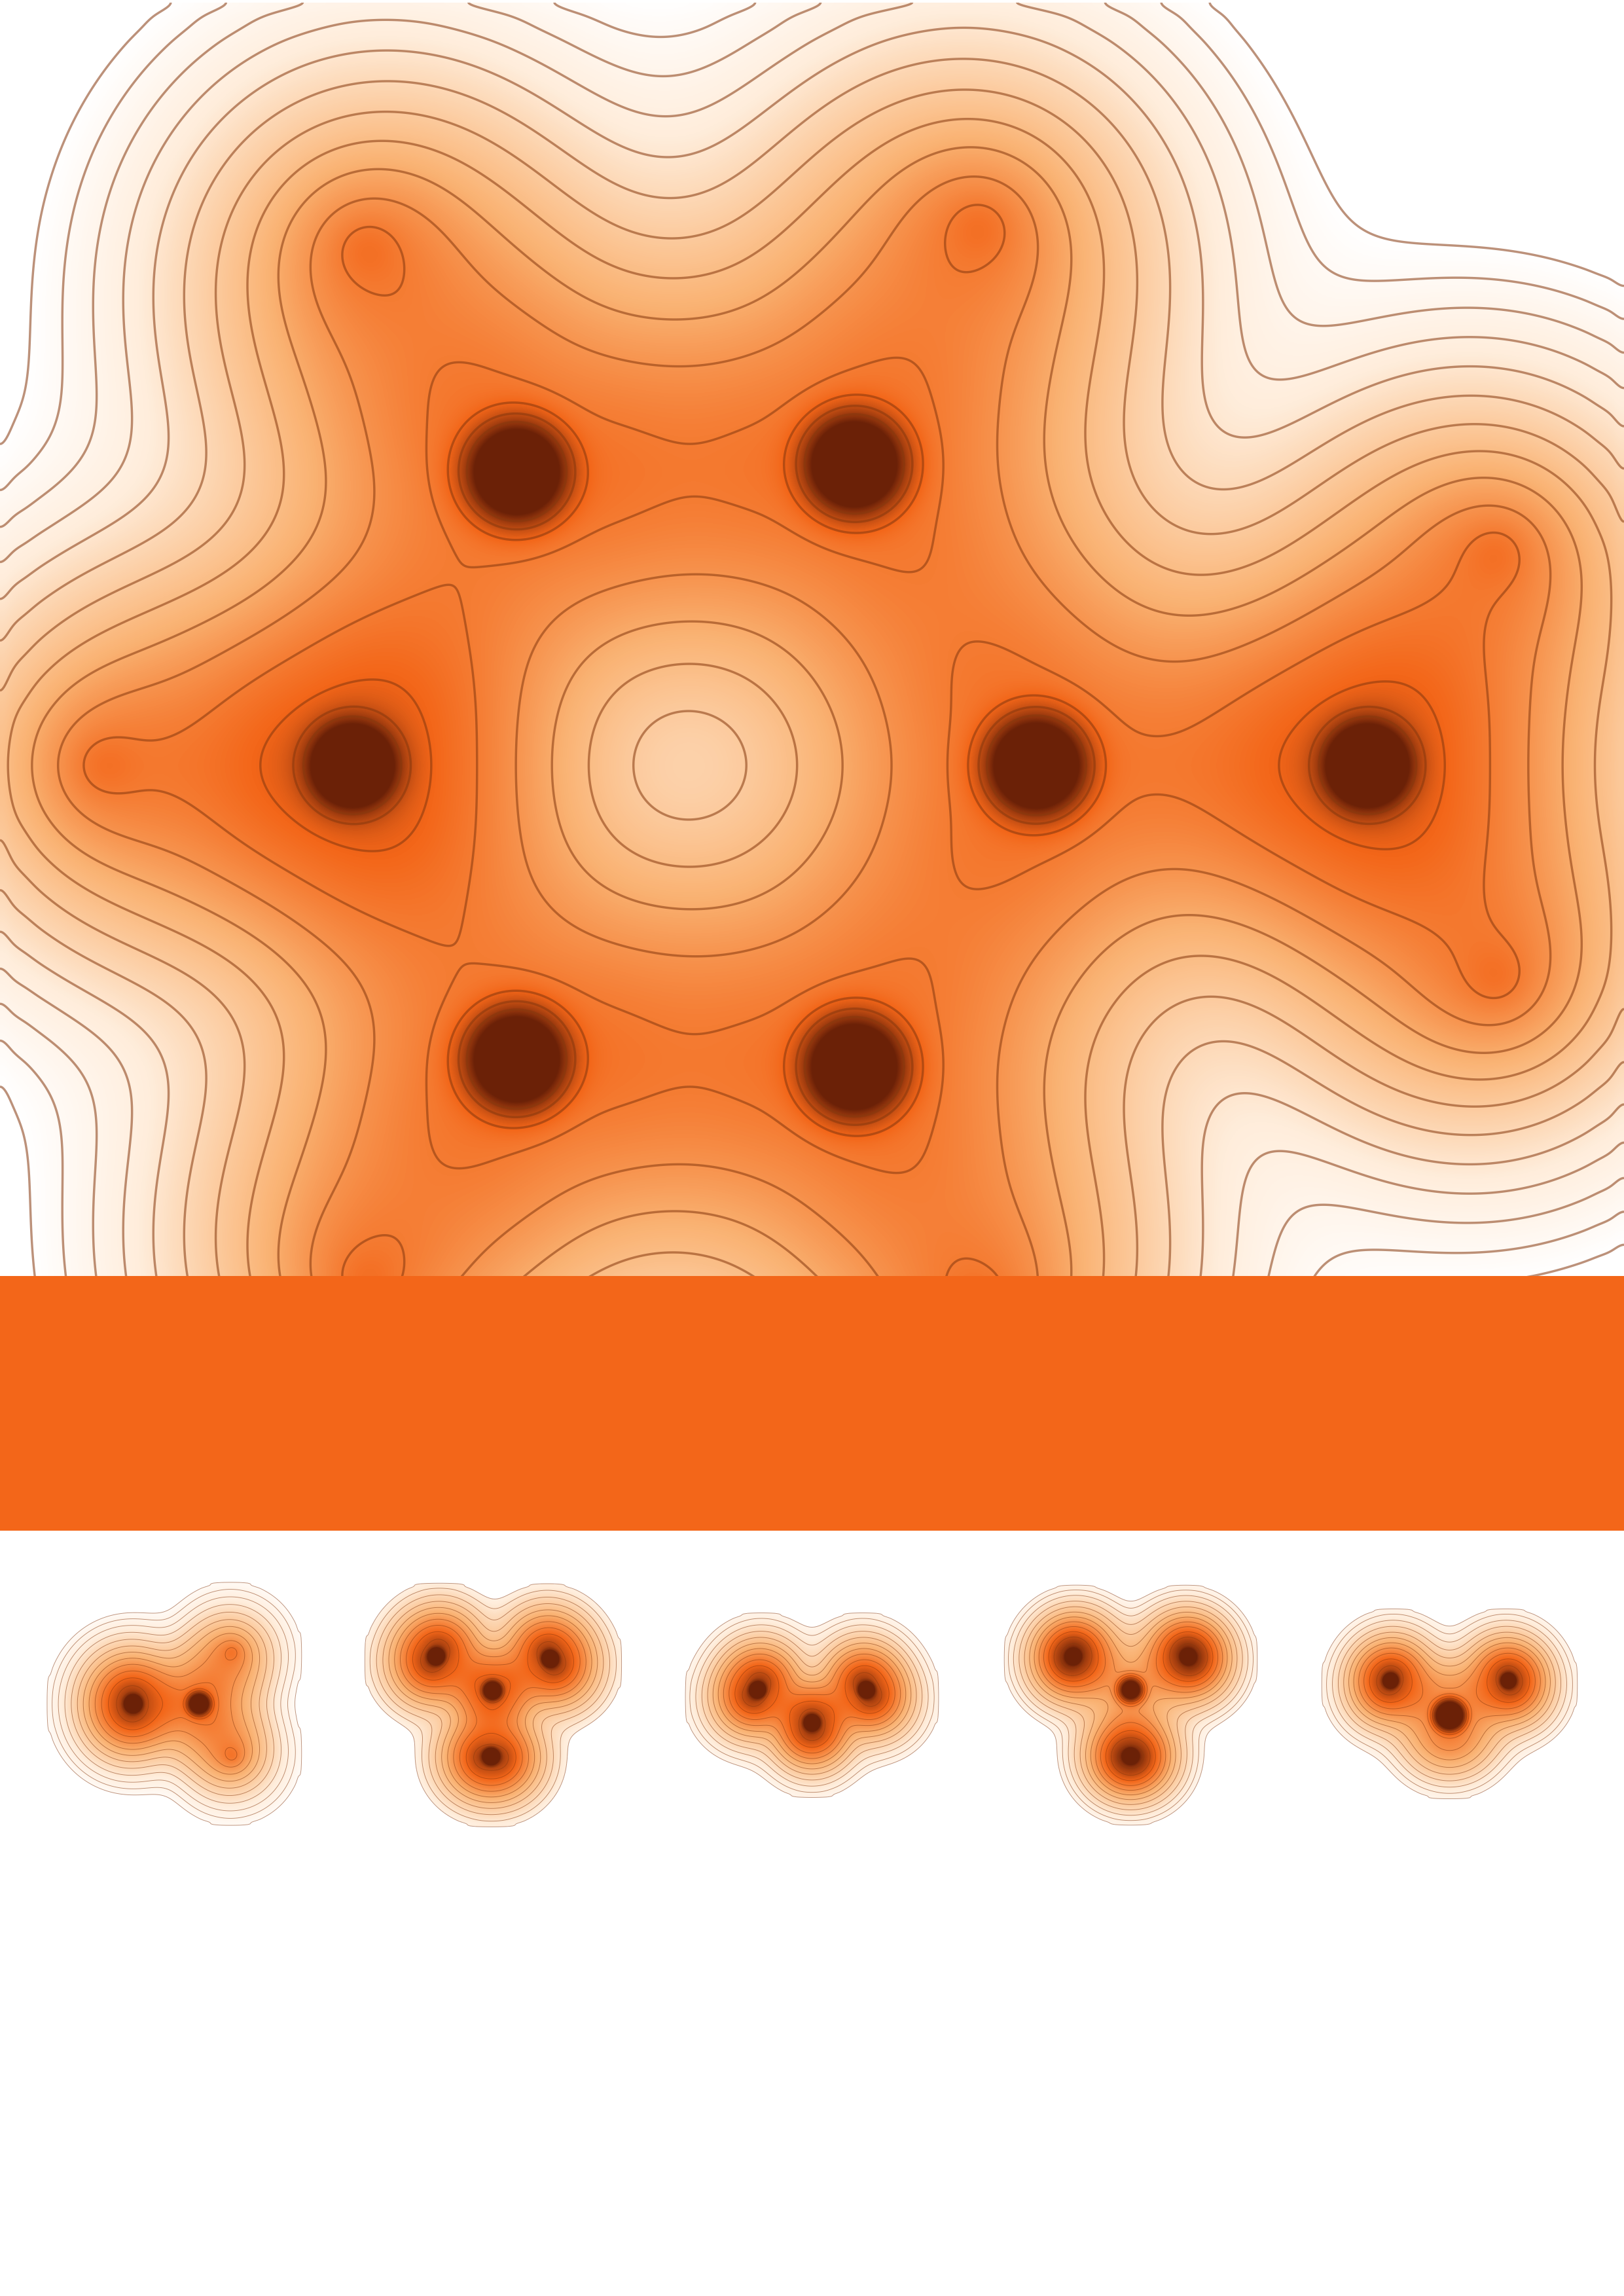
\includegraphics[width=\paperwidth,height=\paperheight]{figures/cover.png}};
	\node[anchor=west, inner sep=0pt, text width=0.86\paperwidth, align=left, text=white, font=\sffamily]
		at ($(current page.north west)!0.611!(current page.south west) + (0.07\paperwidth,0)$)
		{{\fontsize{34}{38}\selectfont\bfseries ECCE by Example\par}\vspace{8pt}
		 {\large Worked calculations with the Extensible Computational Chemistry Environment\par}};
	\node[anchor=south west, inner sep=0pt, font=\sffamily\huge\bfseries]
		at ($(current page.south west) + (0.07\paperwidth,0.07\paperheight)$) {CA Ohlin};
	\node[anchor=south east, inner sep=0pt, font=\sffamily\Large, text=ocre]
		at ($(current page.south east) + (-0.07\paperwidth,0.07\paperheight)$) {For ECCE \ecceversion};
\end{tikzpicture}
\null\newpage

\thispagestyle{empty}
~\vfill
\noindent Copyright \copyright\ 2026 CA Ohlin\\[6pt]
\noindent This book is licensed under the Creative Commons Attribution-NonCommercial-ShareAlike 4.0 International licence (CC BY-NC-SA 4.0), \url{https://creativecommons.org/licenses/by-nc-sa/4.0/}. It may be copied, adapted and shared for non-commercial purposes, with credit, under the same licence.\\[6pt]
\noindent The chapters were drafted with AI assistants (Claude, by Anthropic), which wrote text, ran calculations and made figures under the author's direction. The author reviews the content and is responsible for it.\\[6pt]
\noindent Cover image: the water dimer, calculated with ECCE-QM at B3LYP-D3(BJ)/def2-TZVP (the example \emph{h2o\_dimer} in the General Chemistry examples, Intermolecular interactions; Chapter~\ref{sec:hydrogen-bond}). All maps lie in the plane through the oxygen O1, its hydrogen H2 and the oxygen O4 of the other molecule. Top: molecular orbital 6; blue and orange are its two signs and the grey lines its nodes. Below, from the left: the total electron density, with logarithmic contours, and molecular orbitals 3, 4 and 8. The values are those of ECCE's Density Map; the colour fill was added for the cover.\\[6pt]
\noindent ECCE is free software, available from \url{https://github.com/FriendsofECCE/ECCE}. The screenshots in this book were taken with ECCE \ecceversion.


\pagestyle{empty}
\tableofcontents

\pagestyle{fancy}
\cleardoublepage

\mainmatter

\chapter*{About this book}
\addcontentsline{toc}{chapter}{About this book}
Each chapter of this book is one calculation carried out in ECCE from start to finish: the question it answers, what ECCE shows, a numbered procedure and the results. The purpose of the book is to show how ECCE is used for real work. Where a chapter's calculation is also in one of ECCE's example sets, the chapter says so, and the finished calculation can be opened and compared at any step.

The procedures use the menus and panels of ECCE \ecceversion; menu paths are written as \menu{Tools > Diffraction...}, buttons and fields as \ctrl{Calculate}, and commands as \cmd{ecce-xrd}. Everything a procedure does in the windows can also be done from the command line, and AGENTS.md in ECCE's documentation lists the commands.


The Teaching part is written for teachers. Each of its chapters takes a classical discovery or a core concept of chemistry, from the shells of the atom to Photograph 51, and shows how a calculation in ECCE makes it visible in a lecture or a demonstration: what to show, in which order, what the numbers mean and where the picture can mislead.


% Parts and chapters: chapters/plan.tex, written by chapters.py (make plan).
% Written by chapters.py: edit the PLAN there, not this file.
\part{Getting started}
\chapter{Your first calculation: water}
\label{ch:first-calculation}
\index{Builder}
\index{Calculation Editor}
\index{Launcher}
\index{Viewer}
\index{ECCE-QM}
\index{ORCA}
\index{Run states}
\index{Properties list}
\eccexample{Examples > Getting Started > ecceqm-water}
\helppage{first-calculation}
\helppage{example-calculations}
\helppage{viewer-panels}
\helppage{run-states}
\XXX[ chapter to be written]

\section{Background}

\section{What ECCE shows}

\section{Procedure}

\section{Results}

\section{Coupling with other codes}
% What feeds this calculation (a cheaper screen, a structure from another code)
% and what it feeds (refinement, a property from the code best at it); which
% steps a workflow or recipe automates and which are a manual hand-off.


\chapter{Organising calculations}
\label{ch:organizer}
\index{Organizer}
\index{Projects}
\index{Annotations}
\index{Move to...}
\index{Copy to...}
\index{Checks table}
\index{Re-Parse Outputs}
\index{Excluded calculations}
\eccexample{Examples > Getting Started}
\helppage{organizer-menus}
\helppage{rename-and-move}
\helppage{checks-table}
\helppage{reparse-outputs}
\helppage{excluded}
\XXX[ chapter to be written]

\section{Background}

\section{What ECCE shows}

\section{Procedure}

\section{Results}


\chapter{Running on this computer}
\label{ch:machines}
\index{Machines!this computer}
\index{localhost}
\index{Launcher}
\index{Run states}
\index{Codes!installing}
\eccexample{Examples > Getting Started}
\helppage{machines}
\helppage{running-codes-on-linux}
\helppage{running-codes-on-macos}
\helppage{running-codes-on-windows}
\XXX[ chapter to be written]

\section{Background}

\section{What ECCE shows}

\section{Procedure}

\section{Results}

\section{Coupling with other codes}
% What feeds this calculation (a cheaper screen, a structure from another code)
% and what it feeds (refinement, a property from the code best at it); which
% steps a workflow or recipe automates and which are a manual hand-off.


\chapter{Running on clusters and supercomputers}
\label{ch:hpc}
\index{HPC}
\index{Clusters}
\index{Supercomputers}
\index{Register Machines}
\index{Queues}
\index{Slurm}
\index{PBS}
\index{HTCondor}
\index{Allocations}
\index{Projects (accounts)}
\index{ssh}
\index{ssh keys}
\index{Two-factor authentication}
\index{Scratch}
\index{Job scripts}
\index{Modules (environment modules)}
\index{Launch Selected}
\index{Reconnect}
\index{ecce-launch}
\index{ecce-reconnect}
\index{Moving a job to another machine}

\checkedwith{9.5.3-dev}{4c8b4b851}
\helppage{register-machines}
\helppage{allocations}
\helppage{launch-selected}
\helppage{reconnect-selected}
A laptop is fine for a water molecule, but most research calculations need more cores, more memory and more time than a desktop computer offers, and they go to a cluster: a shared machine run by a university or a national centre, where jobs wait in a queue and are charged to a project's allocation. Running a code there by hand means logging in, copying files, writing a batch script in the queue manager's own language, submitting it, watching the queue and copying the results back. ECCE does all of this itself once the cluster has been described to it, and this chapter shows how. The examples use Kebnekaise at HPC2N in Umeå, a Slurm cluster with environment modules, which is typical of the machines most of us will meet.

\section*{This requires}
An account on a cluster that you can reach with ssh, a project to charge jobs to, and the codes you want to run installed there (on most clusters as environment modules). Nothing needs to be installed on the cluster for ECCE itself.

\section{What ECCE needs to know}
\index{Machine Registration}
For a cluster, ECCE needs the same three things as for the computer we sit at (Chapter~\ref{ch:machines}), that the machine exists, where the codes are, and which queues it has, plus two more: how to log in, and what the batch script should contain. All of it is entered once, in \menu{Tools > Register Machines...}, and stored in a few small files in \texttt{\textasciitilde/.ECCE}. Most settings come in two layers. A \emph{site setting} belongs to the installation and is shared by everyone who uses it, so that a teacher or an administrator can describe a cluster once for a whole class. A \emph{user setting} is your own, and it \emph{replaces} the site setting rather than being added to it. The small tag next to each value says which applies (\emph{from site}, \emph{your value} or \emph{not set}).

\section{Registering the cluster}
\index{Register Machines!new cluster}
\begin{enumerate}
	\item In \menu{Register Machines}, choose \menu{New Machine}. On the \menu{Machine} tab, enter the login host in \menu{Machine} (for Kebnekaise, \texttt{kebnekaise.hpc2n.umu.se}) and a short name for the list in \menu{Name}, set \menu{Nodes} and \menu{Processors}, and enter your user name, your project's account and a run directory on the cluster.
	\item On the \menu{Queues} tab, choose the \menu{Queue manager} (Slurm here) and tick \menu{Allocation accounts used}, since every job on Kebnekaise is charged to a project. Rather than typing the queues, choose \menu{Discover queues...}: ECCE logs in, runs \texttt{sinfo}, and fills in each partition with its processor, wall-time and memory limits. Tick the ones you want, add them, and enter the defaults yourself, since discovery leaves them empty.
	\item On the \menu{Codes} tab, select each code you will run. On a cluster with environment modules, enter the modules the code needs in \menu{Modules} (the job script then runs \texttt{module load} with them), and either the program's full path in \menu{Program} or press \menu{Find}, which asks the cluster where the program is. Note that \menu{Find} runs only the login setup of the \menu{Connection} tab before it searches, not the code's \menu{Modules}, so a program that exists only after a \texttt{module load} is found only if that command is in the login setup; otherwise type its path.
	\item Choose \menu{Save}.
\end{enumerate}
\index{Discover queues}\index{Modules (environment modules)}

Two buttons check the description before a real job depends on it. \menu{Preview job script...} on the \menu{Job script} tab shows the script ECCE would write for a code and a queue, with each line labelled by the tab that produced it, so that a wrong module or a missing account line is seen at once. \menu{Test submission...} on the \menu{Queues} tab sends a script with this queue's request lines and no calculation to the queue manager, which for Slurm is \texttt{sbatch --test-only}, and reports whether it would be accepted. Note that this is the moment to find out that an account is spelt wrongly or a partition needs a quality-of-service line, rather than after a job has waited an hour in the queue.

The request lines themselves, the \texttt{\#SBATCH} lines at the top of the script, usually come from the site and are right as they are. Where your account needs one more line, \menu{Copy site setting} puts the site's lines in your own box, where you add the line and save; the words that start with \texttt{\$}, such as \texttt{\$wallTime} and \texttt{\$totalprocs}, are placeholders that ECCE fills in for each job.

\section{Logging in}
\index{ssh}\index{ssh keys}\index{Two-factor authentication}
ECCE logs in with ssh. If you have an ssh key set up for the cluster, as most of us do, ECCE uses it and asks for nothing; otherwise it asks for the password in its own window, and can remember it in the computer's password store (the Keychain on macOS, the Credential Manager on Windows, a keyring on Linux) if you tick \menu{Remember on this computer}. One login is shared by everything ECCE does on that machine during the session, the launch, the job monitoring, the transfer of results and the Allocations window. A cluster that requires a two-factor login ECCE cannot answer can still be used through the \texttt{dummy} machine, for which ECCE writes the input and the job script and stops, leaving the submission and the import of the results to you (\menu{File > Import Calculation from Output File...}, Chapter~\ref{ch:structures}).

\section{Launching, waiting and coming back}
\index{Launcher}\index{Reconnect}\index{Launch Selected}
In the Launcher, choose the cluster in \menu{Machine:}. The Launcher now asks for the queue, the number of nodes and cores, the memory and the wall time, and, if the machine has more than one allocation profile, which allocation to charge. \menu{Launch} copies the input and the job script to the run directory, submits the job and follows it. While the job waits in the queue the calculation is \emph{Submitted}; once it starts it is \emph{Running}, and the Progress box shows its energies and steps as the output grows, just as on \texttt{localhost}. The calculation's summary in the Organizer shows the account the job was charged to and how much of its wall time is left.

Cluster jobs often run for longer than we keep a laptop open. Closing ECCE does not affect the job, but ECCE stops following it, and the calculation is shown as \emph{Waiting for Login}. At the next start ECCE takes it up again, or at once with \menu{Run Mgmt > Reconnect Selected...}, which can reconnect many calculations in one step; when the job has finished in the meantime, its output is fetched and read as usual. \emph{Running?} means that the connection was lost for the moment while the job was running.

Many calculations at once are launched with \menu{Run Mgmt > Launch Selected...}, which uses the settings stored in each calculation and can send them all to another machine, so that a series prepared and tested on \texttt{localhost} can be moved to the cluster unchanged. The same is available from a terminal and to scripts as \texttt{ecce-launch on=MACHINE queue=QUEUE wall=H:MM} followed by the calculations (Chapter~\ref{ch:scripting}).
\index{ecce-launch}\index{ecce-reconnect}\index{Moving a job to another machine}

\section{Allocations}
\index{Allocations}
A cluster charges each job to a project, and running out of hours halfway through a series is avoidable. \menu{Tools > Allocations...} in the Organizer shows, for each machine and account, how much of the allocation has been used, as the cluster itself reports it (on Slurm machines by default with \texttt{sshare}, and at HPC2N and the other NAISS centres with \texttt{projinfo}, entered as the machine's \menu{Allocation command} on the \menu{Connection} tab). If you have more than one allocation on the same cluster, for example a course allocation and a research project, each gets its own \emph{allocation profile} with its account, directories and default queue, and the Launcher lets you choose between them; a calculation remembers which profile it was launched with.

\section{Coupling with other codes}
A cluster is where the expensive end of a coupled chain runs. The usual pattern is to screen and optimise cheaply on \texttt{localhost}, with xTB or ECCE-QM, and to send only the few structures that matter to a density functional or coupled-cluster calculation on the cluster, choosing the cluster in the Launcher of the new calculation made with \menu{New from This} (Chapter~\ref{ch:coupling}). Nothing else in the calculation changes when it moves between machines.

\chapter{Registering codes: programs, environments and new codes}
\label{ch:code-registration}
\index{Code registration}
\index{Registering a code}
\index{Codes!environment variables}
\index{Codes!job script}
\index{EDML}
\index{Parsers}
\index{Input generators}
\index{Adding a new code}
\index{Pseudopotential paths}


\XXX[ chapter to be written]

\section{Background}

\section{What ECCE shows}

\section{Procedure}

\section{Results}

\section{Coupling with other codes}
% What feeds this calculation (a cheaper screen, a structure from another code)
% and what it feeds (refinement, a property from the code best at it); which
% hand-off is made (usually by hand: a new calculation from this one's
% structure or orbitals in another code); a workflow only where it pays.


\chapter{Building and importing structures}
\label{ch:structures}
\index{Builder!import}
\index{Structure Library}
\index{SMILES}
\index{Add from SMILES}
\index{Replace Group}
\index{Clean}
\index{Constraints}
\index{Dummy atoms}
\index{Importing calculations}
\eccexample{Examples > Getting Started}
\helppage{importing-a-structure}
\helppage{importing-a-calculation}
\helppage{bonds-and-clean}
\helppage{constraints-and-dummy-atoms}
\XXX[ chapter to be written]

\section{Background}

\section{What ECCE shows}

\section{Procedure}

\section{Results}


\chapter{ECCE from scripts and AI assistants}
\label{ch:scripting}
\index{Command line}
\index{AGENTS.md}
\index{ecce-rerun}
\index{ecce-reparse}
\index{Series of calculations}
\index{AI assistants}
\eccexample{Examples > Getting Started}
\helppage{scripting-and-ai}
\helppage{new-series}
\XXX[ chapter to be written]

\section{Background}

\section{What ECCE shows}

\section{Procedure}

\section{Results}

\section{Coupling with other codes}
% What feeds this calculation (a cheaper screen, a structure from another code)
% and what it feeds (refinement, a property from the code best at it); which
% steps a workflow or recipe automates and which are a manual hand-off.



\part{Methods}
\chapter{Coupling computations: screening, refinement and hand-offs between codes}
\chaptermark{Coupling computations}
\label{ch:coupling}
\index{Coupling computations}
\index{New from This}
\index{Screening}
\index{Refinement}
\index{Hand-offs between codes}
\checkedwith{9.5.3-dev}{5b6fbfa5e}
\helppage{crest}
\helppage{xtb}
\helppage{new-series}

Most research problems are too large for the method that would be trusted to give the answer and too open for a single guess to be enough. The usual way out is to let a cheap method look at many candidates and an expensive one look at a few, and to let each property come from the code that is best at it. ECCE stores every calculation with its structure, its results and the setup that produced them, so that the structure leaving one code can enter the next without being retyped, and without a file format in between. This chapter shows how such hand-offs are made, with one worked example, the conformers of ibuprofen taken from CREST through xTB to ORCA, and then describes the same pattern for periodic models, for molecular dynamics and for a structure that several codes treat in turn.
\index{Codes!CREST}\index{Codes!xTB}\index{Codes!ORCA}

Coupling in this sense is done by hand, one calculation made from another, in the Organizer and the Builder. Chapter~\ref{ch:workflows} describes how a chain that is run often can be drawn once and launched as a unit; the steps are the same, and doing them by hand a few times is the best way to see what the chain does.

\section{Background}
\index{Screening funnel}\index{Multi-level calculations}

\subsection{The screening funnel}
A flexible molecule has no single structure. Ibuprofen, \chem{C13H18O2}, has five rotatable single bonds, in the isobutyl group, between the ring and the propionic acid group, and in the carboxyl group, and each combination of their rotations is a conformer. A conformer search with a tight-binding method \cite{pracht2020,bannwarth2019} finds the local minima in minutes, but the energies of tight-binding methods are good enough to separate conformers only roughly, and a density functional calculation on every conformer is the cost that the search was meant to avoid. A funnel solves this by passing a growing amount of effort to a shrinking set of structures: a force field or tight-binding search generates and ranks the conformers, a better tight-binding method re-optimises the lowest ones, and a composite density functional method refines the structure that is left (Fig.~\ref{fig:coupling-funnel}).

Three points decide whether a funnel works. The cheap step has to keep every structure that the expensive step could prefer, which is why the window of the search and the number of structures passed on are generous. The ranking at one level does not have to agree with that of the next in detail, only to put the structures the next level prefers within reach; the example below shows what this looks like. And the energies of different methods are never put on one scale. The funnel compares structures and orders, and each method's energies are read against that method's own lowest value.
\index{Energies!comparison between methods}

\begin{figure}[htb]
	\centering
	\begin{tikzpicture}[node distance=7mm]
		\node[calcbox, text width=0.80\linewidth] (start) {\textbf{xTB}, GFN2-xTB, Geometry\\ the structure built from SMILES \hfill 1 structure};
		\node[calcbox, text width=0.80\linewidth, below=of start] (crest) {\textbf{CREST}, GFN-FF, Conformer Search, 6~kcal/mol window\\ the conformer ensemble \hfill 21 conformers};
		\node[calcbox, text width=0.66\linewidth, below=11mm of crest] (xtb) {\textbf{xTB}, GFN2-xTB, Geometry\\ the distinct conformers re-optimised \hfill 8 structures};
		\node[calcbox, text width=0.52\linewidth, below=of xtb] (sp) {\textbf{ORCA}, r2SCAN-3c, Energy\\ ranking on the xTB structures \hfill 8 energies};
		\node[calcbox, text width=0.38\linewidth, below=of sp] (opt) {\textbf{ORCA}, r2SCAN-3c, Geometry\\ the refined structure \hfill 1 structure};
		\draw[handoff] (start) -- node[handofflabel, right=2pt] {final geometry as the start} (crest);
		\draw[handoff] (crest) -- node[handofflabel, right=2pt] {\cmd{ecce-ensemble pick}, then\\ \menu{New Calculation from Selected...}} (xtb);
		\draw[handoff] (xtb) -- node[handofflabel, right=2pt] {\cmd{ecce-series} with an ORCA template} (sp);
		\draw[handoff] (sp) -- node[handofflabel, right=2pt] {one conformer, from its xTB structure} (opt);
	\end{tikzpicture}
	\caption{The screening funnel of this chapter for ibuprofen. Each box is one kind of calculation in ECCE, with its code, theory and run type and the number of structures it handles; each arrow is the hand-off from one to the next and the ECCE route for it. The effort per structure grows downwards and the number of structures shrinks.}
	\label{fig:coupling-funnel}
	\index{Screening funnel!flow chart}
\end{figure}

\subsection{Other hand-offs}
The funnel is one of four patterns that the rest of the book uses.
\begin{itemize}
	\item \emph{Multi-level calculations}: the geometry at a lower level, an energy or a property at a higher one.
	\item \emph{Across scales and models}: parameters or charges from a quantum calculation into molecular dynamics, snapshots from a trajectory into quantum calculations, a periodic model into a cluster for a molecular code.
	\item \emph{One structure, each property from the best code}: the same coordinates in several programs, each asked what it does best.
\end{itemize}

\section{What ECCE shows}
\index{Conformers panel}\index{Properties list!Conformers}\index{Geometry Trace}
\index{Properties list!Geometry Trace}

A finished CREST calculation has a \menu{Conformers} panel in the \menu{Properties} list of the Builder, under \menu{Geometry}. It has one row for each conformer in CREST's final list, lowest first, with a picture of the structure, the rank, the energy relative to the lowest one in kcal/mol, and the Boltzmann population in percent at 298.15~K. Clicking a row shows that structure in the 3-D view, ticking several rows and choosing \menu{New Calculation from Selected...} asks once for the code and makes one calculation for each of them, with the structure of the row, the Geometry Optimization run type and the charge and multiplicity of the CREST calculation. Below the table a plot of energy against rank marks the chosen structure.
\index{Conformers panel!New Calculation from Selected}\index{Conformers panel!Export .csv}

A conformer search from a molecule with many near-degenerate conformers returns many structures that differ by a rotation of a methyl group. The command \cmd{ecce-ensemble pick} reads the same stored ensemble and merges members whose heavy atoms lie within a given distance after a fit (\SI{0.5}{\angstrom} by default), which gives a list of distinct structures. Each pick is also checked against the input structure, for a change of protonation or of bound ions, and the report says if the check fails.
\index{Commands!ecce-ensemble}\index{Distinct conformers}

For the step from xTB to ORCA, ECCE makes a calculation from a template, a calculation whose code, theory, run type, basis set and launch settings are wanted, with a list of structures or stored calculations as the sources of the geometry. The command is \cmd{ecce-series}, and a stored calculation brings its own final geometry, charge and multiplicity.
\index{Commands!ecce-series}\index{New Series}\index{Template calculation}
In a workflow the same hand-off is the \menu{New step} window, which takes the final geometry of the selected box into a step of another code (Chapter~\ref{ch:workflows}).

\section{Procedure}
\index{CREST!conformer search}\index{Conformer search}

The calculation uses ibuprofen, built from the SMILES string \texttt{CC(C)Cc1ccc(cc1)C(C)C(=O)O}. Everything is done in one project folder, so that the calculations are next to one another in the Organizer and each can be chosen as the source of the next.
\begin{enumerate}
	\item In the Organizer, make a project and, with \menu{File > New}, an xTB calculation. In the Builder choose \menu{Tools > Add from SMILES...} and enter the string, and set the run type to Geometry with the theory GFN2-xTB.
	\index{Tools menu!Add from SMILES...}\index{SMILES}
	\item Launch the calculation. CREST starts from an optimised structure and fails from an unoptimised one, which is why this step is first.
	\item Click the \menu{CREST} code button in the code bar to make a CREST calculation and give it the structure of the xTB result, with the run type \menu{Conformer Search} and the theory \menu{GFN-FF}. Leave the \menu{Energy window} at 6~kcal/mol, and launch.
	\index{CREST!Theory}\index{CREST!Energy window}\index{GFN-FF}
	\item When the calculation is complete, open it in the Builder and choose \menu{Properties > Geometry > Conformers}. Sort the table by the column heads if wanted. To keep the distinct conformers only, run \cmd{ecce-ensemble pick} on the calculation with the number of picks wanted, here eight.
	\item In the table ctrl-click the conformers to be refined and choose \menu{New Calculation from Selected...}. Choose xTB; the new calculations are Geometry optimisations, named after the CREST calculation with \texttt{\_conf} and the rank. Select them and choose \menu{Run Mgmt > Launch Selected...}.
	\index{Run Mgmt menu!Launch Selected...}
	\item Make the ORCA template: a calculation with the code ORCA, the theory \menu{DFT}, the functional \menu{r2SCAN-3c} in \menu{Theory Details}, the run type Geometry (or Energy for a ranking only) and the cores and machine to be used. The composite carries its own basis set, so no basis set is chosen.
	\index{r2SCAN-3c}\index{Composite methods}\index{ORCA!Theory Details}
	\item Run \cmd{ecce-series} with the template, the folder and the xTB calculations as sources, then select the new calculations and launch them as before.
	\item To compare the structures before and after a step, select several rows of the \menu{Conformers} panel; they are fitted onto the first one and the key under the table lists the heavy-atom RMSD of each.
	\index{Conformers panel!Superposing members}\index{RMSD}
\end{enumerate}

The calculations of this chapter were made headless, through ECCE's own Launch with decks written by the same scripts as in the Calculation Editor, in an isolated data folder (ECCE 9.5.3-dev, \cmd{nice} level 19, at most four cores). The harness stores the structure and deck of each calculation and not the Calculation Editor setup, so the xTB and ORCA calculations were made one by one with the structures of the picked conformers, which is what steps 5 to 7 produce; \cmd{ecce-ensemble pick} was run as described. The steps in the Organizer and Builder follow the help pages of ECCE; step 5 to 7 were not driven through the windows for this chapter.

\section{Results}
\index{Ibuprofen}

\subsection{CREST and GFN-FF}
The GFN2-xTB optimisation of the SMILES structure took 33~s and the CREST search with GFN-FF, on two cores, 236~s. CREST kept 21 conformers within 6~kcal/mol of the lowest one. The Conformers panel (Fig.~\ref{fig:coupling-conformers}) shows the lowest first, and the first four are within 0.12~kcal/mol of one another, a spread that no method of this class can resolve. \cmd{ecce-ensemble pick} with a merge distance of \SI{0.5}{\angstrom} returned the same first eight as separate structures, so all eight differ in the heavy-atom skeleton by more than that distance, and each differs from the lowest by \SIrange{0.8}{1.7}{\angstrom} in heavy-atom RMSD.
\index{Heavy-atom RMSD}

\begin{figure}[htb]
	\centering
	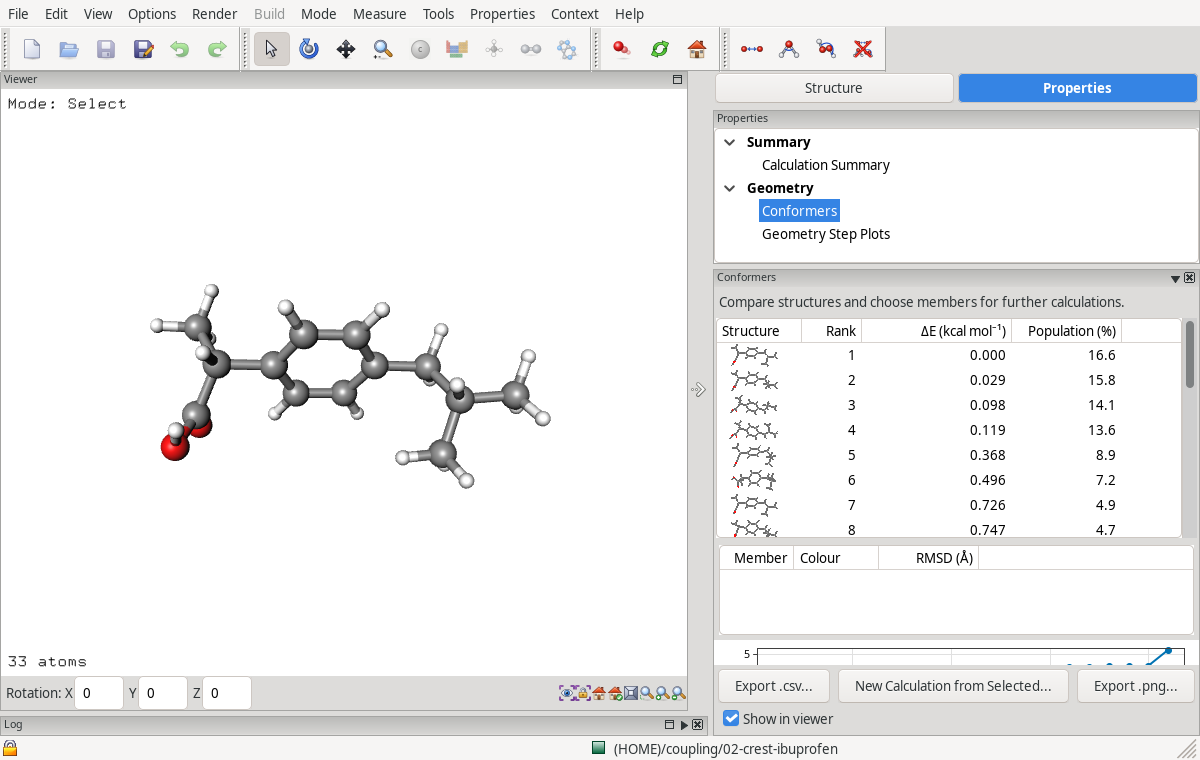
\includegraphics[width=\linewidth]{coupling/crest-conformers.ecce-9.5.3-dev.png}
	\caption{The \menu{Conformers} panel for the CREST search on ibuprofen. The rows give rank, relative energy and population within GFN-FF; the 3-D view shows the lowest conformer on a white background.}
	\label{fig:coupling-conformers}
\end{figure}

\subsection{xTB and the ranking}
Each of the eight picks was optimised with GFN2-xTB (\SIrange{33}{48}{\second} each) and then given a single-point energy with ORCA and r2SCAN-3c \cite{grimme2021} on the xTB structure (\SIrange{33}{102}{\second} on four cores), so that the order of the conformers at the three levels could be set side by side. Table~\ref{tab:coupling-rank} gives the order and, for each method, the energy relative to that method's own lowest conformer. The columns are not to be subtracted from one another.
\index{Ranking of conformers}

\begin{table}[htb]
	\centering
	\caption{Eight distinct conformers of ibuprofen at three levels. Each energy column is relative to the lowest conformer of that column, in kcal/mol; conformer 3 is the lowest at the xTB level and conformer 4 at the r2SCAN-3c level.}
	\label{tab:coupling-rank}
	\begin{tabular}{rrrrrrr}
		\toprule
		Conformer & \multicolumn{2}{c}{GFN-FF} & \multicolumn{2}{c}{GFN2-xTB} & \multicolumn{2}{c}{r2SCAN-3c} \\
		 & rank & rel. & rank & rel. & rank & rel. \\
		\midrule
		1 & 1 & 0.00 & 3 & 0.01 & 2 & 0.09 \\
		2 & 2 & 0.03 & 2 & 0.01 & 4 & 0.11 \\
		3 & 3 & 0.10 & 1 & 0.00 & 3 & 0.10 \\
		4 & 4 & 0.12 & 4 & 0.02 & 1 & 0.00 \\
		5 & 5 & 0.37 & 6 & 0.47 & 6 & 0.64 \\
		6 & 6 & 0.50 & 5 & 0.45 & 5 & 0.60 \\
		7 & 7 & 0.73 & 8 & 0.75 & 7 & 1.56 \\
		8 & 8 & 0.75 & 7 & 0.74 & 8 & 1.60 \\
		\bottomrule
	\end{tabular}
\end{table}

Inside each of three groups, conformers 1 to 4, 5 and 6, and 7 and 8, the order changes from one method to the next, and the differences within a group are a few hundredths of a kcal/mol at the xTB level and about a tenth at the r2SCAN-3c level, so the order inside a group has no meaning at any of the levels. The groups themselves keep their order at all three: the first four are always lowest, the pair 5 and 6 next, the pair 7 and 8 highest. This is the situation for which the funnel is designed. A cut at the lowest conformer of the cheap method would have dropped conformer 4, which the most expensive method puts first, and a cut after four conformers would have kept it. Passing on several conformers, and not one, costs a few minutes here.
\index{Funnel!choice of the number of structures}

The group structure is itself a result for ibuprofen: the four lowest conformers are separated from the rest by a gap that is larger than the differences inside them, and at the GFN-FF level the populations of all eight conformers are above 4 percent, so that a Boltzmann average over this molecule at room temperature would need more than the lowest one. Whether the gap persists at a higher level is a question for a calculation at that level and is not settled by this table.

\subsection{Refinement with ORCA}
The conformer that xTB put lowest, conformer 3, was optimised with r2SCAN-3c in ORCA from its xTB structure (Fig.~\ref{fig:coupling-orca}). The optimisation converged in 10 steps and \SI{341}{\second} on four cores, and moved the heavy atoms by \SI{0.096}{\angstrom} (RMSD after a fit). In the carboxyl group the C=O bond is \SI{1.201}{\angstrom} in the xTB structure and \SI{1.209}{\angstrom} after the optimisation, the C--O single bond \SI{1.340}{\angstrom} and \SI{1.357}{\angstrom}, and the O--H bond \SI{0.971}{\angstrom} in both. A step from tight-binding to a density functional therefore changes bond lengths by a few hundredths of an ångström and leaves the conformer as it was, which is what makes the hand-off of the structure sensible.
\index{Geometry optimisation!ORCA}\index{Bond lengths!carboxyl group}

\begin{figure}[htb]
	\centering
	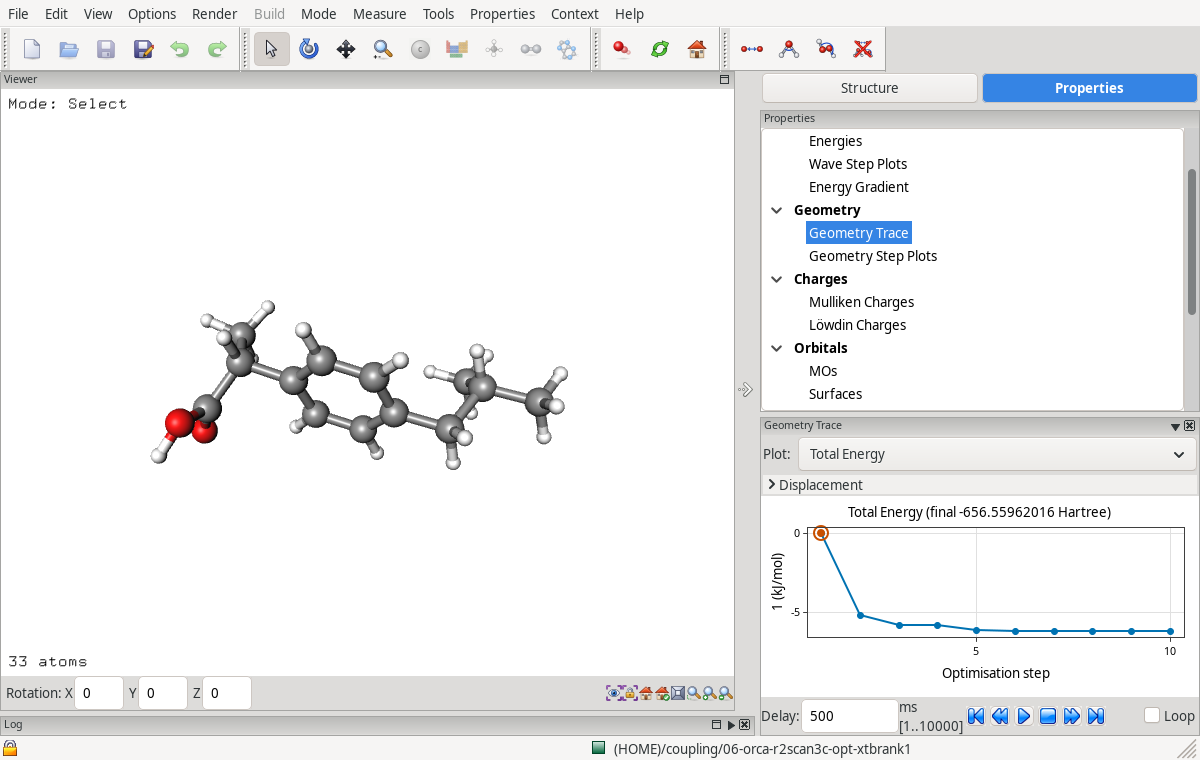
\includegraphics[width=\linewidth]{coupling/orca-opt-trace.ecce-9.5.3-dev.png}
	\caption{The ORCA r2SCAN-3c optimisation of ibuprofen conformer 3 in the Builder, with the \menu{Geometry Trace} panel plotting the energy of each optimisation step relative to the first.}
	\label{fig:coupling-orca}
\end{figure}

The calculations are in the repository of this book under \texttt{calculations/coupling}, in the order of the funnel: \texttt{01-xtb} the starting structure, \texttt{02-crest} the search, \texttt{03-xtb} the eight re-optimisations, \texttt{05-orca} the eight single points and \texttt{06-orca} the optimisation. A real project would stop earlier or later, depending on what the structure is wanted for. Frequencies and free energies, for instance, would be one more calculation on the last structure, in the same code, from \menu{New from This > Continue from Last Geometry}.
\index{New from This!Continue from Last Geometry}

\section{Across scales and from periodic models}
\index{Periodic models!to clusters}\index{Cluster models}

The hand-offs below were not run for this chapter. They are what the help pages of ECCE describe, and each is given with the page that describes it so that it can be checked against the version in use.

\emph{A periodic model into a cluster for a molecular code.} ECCE has no command that cuts a cluster out of a periodic structure and caps the cut bonds in one step. The pieces exist in the Builder: \menu{Edit > Select Within Distance...} selects the atoms, or whole molecules, within a distance of the current selection (with an option to keep the original selection), \menu{Edit > Reverse Selection} and \menu{Edit > Delete Selection} remove the rest, and the \menu{Delete Lattice} button of the Periodic Builder removes the cell. \menu{Build > Add Hydrogen} fills open valences from the atom shapes. That works for an organic fragment, but on a cut oxide every added atom needs checking. A new calculation then hands the cluster to a molecular code, for example through \cmd{ecce-series} with a template of that code. The user decides which atoms to keep and how to saturate the surface, and compares the cluster with the periodic model for the property of interest, not for the total energy.
\index{Select Within Distance}\index{Edit menu!Select Within Distance...}\index{Periodic Builder!Delete Lattice}\index{Edit menu!Delete Selection}\index{Edit menu!Reverse Selection}

\emph{A machine-learned potential into a quantum code.} A MACE calculation of a periodic cell or a molecule is cheap enough to optimise a structure first; the help page of the MLP code advises a Geometry run followed by a new calculation from its last structure for the property that needs a minimum. The same step, a new calculation in Quantum ESPRESSO or CP2K from the final geometry, is the hand-off from the machine-learned potential to the quantum code. Chapter~\ref{ch:mlp} describes the potential.
\index{MACE}\index{Codes!MACE}

\emph{Molecular dynamics and quantum chemistry.} A trajectory (a \texttt{.trj} or multi-frame \texttt{.xyz} file) opens in the Builder with \menu{File > Open...}, and a frame that is saved as a structure can be the source of a new calculation by the same route as above. \menu{Edit > Take Coordinates From...} puts the coordinates of chosen atoms of one calculation of the same folder into another that has the same atoms in the same order, with an optional alignment first, which is how a QM-optimised ligand is put back into a larger system.
\index{Take Coordinates From}\index{Trajectories!to quantum chemistry}

\section{One structure, each property from the best code}
\index{Properties!from different codes}

The last pattern needs no new mechanism. One structure, for instance the r2SCAN-3c structure of conformer 3 above, is the source of several calculations that differ in the code: the orbitals and a population analysis in ORCA, a vibrational spectrum from xTB or from ECCE-QM, a dipole moment or a surface from another code, each made from the same stored geometry by \cmd{ecce-series} or by the \menu{New step} window, so that the coordinates are exactly the same in each. Within one code, \menu{New from This > Continue from Final Orbitals} starts the new calculation from the orbitals of the finished one for ORCA, Gaussian 16, NWChem, ECCE-QM, MOPAC, CP2K and Quantum ESPRESSO, which saves iterations for a larger basis set.
\index{Continue from Final Orbitals}\index{Series of calculations}
What each code does best is a question for the chapters of the field in which the property matters. The only rule that the coupling itself adds is the one used in Table~\ref{tab:coupling-rank}: the properties of different codes are read side by side, as structures, orders and quantities of the same kind, and the total energies of different methods are not subtracted.

\section{Where next}
The chapters of the Organic part use the funnel from the CREST search onwards (Chapter~\ref{ch:crest}), and the Inorganic part adds the solvation shell and the counter ions (Chapter~\ref{ch:pom-solvation}). The Materials part takes the periodic route (Chapters~\ref{ch:cp2k}, \ref{ch:mlp} and~\ref{ch:crystals}) and the Biochemistry part the docking funnel (Chapter~\ref{ch:docking}). Chapter~\ref{ch:workflows} shows how to draw a chain once and launch it as a unit.

\chapter{A project done with an AI assistant}
\label{ch:ai-project}
\index{AI assistants}
\index{Claude Code}
\index{AGENTS.md}
\index{ECCE skill}
\index{Series of calculations}


\XXX[ chapter to be written]

\section{Background}

\section{What ECCE shows}

\section{Procedure}

\section{Results}

\section{Coupling with other codes}
% What feeds this calculation (a cheaper screen, a structure from another code)
% and what it feeds (refinement, a property from the code best at it); which
% hand-off is made (usually by hand: a new calculation from this one's
% structure or orbitals in another code); a workflow only where it pays.


\chapter{Workflows and recipes: when to automate a chain}
\label{ch:workflows}
\index{Workflows}
\index{Recipes}
\index{Auto-run}
\index{Launch Ready Steps}
\index{Writing a recipe}
\index{ecce-workflow}
\eccexample{Examples > Workflows}
\helppage{workflows}
\helppage{recipes}
\helppage{writing-a-recipe}
\XXX[ chapter to be written]

\section{Background}

\section{What ECCE shows}

\section{Procedure}

\section{Results}

\section{Coupling with other codes}
% What feeds this calculation (a cheaper screen, a structure from another code)
% and what it feeds (refinement, a property from the code best at it); which
% hand-off is made (usually by hand: a new calculation from this one's
% structure or orbitals in another code); a workflow only where it pays.


\chapter{QSAR: descriptors, PCA and PLS}
\label{ch:qsar}
\index{QSAR}
\index{Descriptors}
\index{PCA}
\index{PLS}
\index{Batch Add from SMILES}
\index{ecce-qsar}
\eccexample{Examples > QSAR}
\helppage{qsar-table}
\helppage{qsar-analysis}
\helppage{batch-from-smiles}
\XXX[ chapter to be written]

\section{Background}

\section{What ECCE shows}

\section{Procedure}

\section{Results}


\chapter{ECCE-QM, the built-in quantum chemistry program}
\label{ch:ecce-qm}
\index{ECCE-QM}
\index{Analytic Hessian}
\index{D3 dispersion}
\eccexample{Examples > Getting Started > ecceqm-water}
\helppage{ecce-qm}
\helppage{ecce-qm-files}
\XXX[ chapter to be written]

\section{Background}

\section{What ECCE shows}

\section{Procedure}

\section{Results}


\chapter{What a calculation approximates: Hartree-Fock, DFT and Jacob's ladder}
\label{ch:hf-dft}
\index{Hartree-Fock}
\index{Density functional theory}
\index{Jacob's ladder}
\index{Electron correlation}
\index{Chemical accuracy}
\index{Model chemistry}
\eccexample{Examples > Computational > H2 dissociation with RHF, UHF and CCSD}

\XXX[ chapter to be written]

\section{Background}

\section{What ECCE shows}

\section{Procedure}

\section{Results}


\chapter{Basis sets: from minimal to the complete basis set limit}
\label{ch:basis-sets}
\index{Basis sets}
\index{Zeta}
\index{Polarisation functions}
\index{Diffuse functions}
\index{Complete basis set limit}
\index{Effective core potentials}
\eccexample{Examples > Getting Started}

\XXX[ chapter to be written]

\section{Background}

\section{What ECCE shows}

\section{Procedure}

\section{Results}


\chapter{Restricted and unrestricted calculations}
\label{ch:restricted-unrestricted}
\index{RHF}
\index{UHF}
\index{ROHF}
\index{Open shells}
\index{Spin contamination}
\eccexample{Examples > Getting Started}

\XXX[ chapter to be written]

\section{Background}

\section{What ECCE shows}

\section{Procedure}

\section{Results}

\section{Coupling with other codes}
% What feeds this calculation (a cheaper screen, a structure from another code)
% and what it feeds (refinement, a property from the code best at it); which
% hand-off is made (usually by hand: a new calculation from this one's
% structure or orbitals in another code); a workflow only where it pays.


\chapter{Choosing methods and checking inputs}
\label{ch:methods-choice}
\index{Composite methods}
\index{r2SCAN-3c}
\index{Verify}
\index{Input checks}
\eccexample{Examples > Getting Started}
\helppage{orca-composite-methods}
\XXX[ chapter to be written]

\section{Background}

\section{What ECCE shows}

\section{Procedure}

\section{Results}


\chapter{Results, reports and citations}
\label{ch:results}
\index{results.h5}
\index{Supporting Information}
\index{Citing ECCE}
\index{Export}
\eccexample{Examples > Getting Started}
\helppage{results-file-format}
\helppage{si-export}
\helppage{citing-ecce}
\XXX[ chapter to be written]

\section{Background}

\section{What ECCE shows}

\section{Procedure}

\section{Results}

\section{Coupling with other codes}
% What feeds this calculation (a cheaper screen, a structure from another code)
% and what it feeds (refinement, a property from the code best at it); which
% steps a workflow or recipe automates and which are a manual hand-off.



\part{Physical chemistry}
% Part overview, set before the part's first chapter.
\checkedwith{9.5.3-dev}{a9b2d49c8}

Physical chemistry asks the questions that every other field relies on: how much energy a reaction releases, how high the barrier is that it has to cross and therefore how fast it goes, how the energy of a molecule changes as its shape changes, what happens to a bond as it is pulled apart, and where the electrons actually are. The chapters of this part answer them one at a time, and because the methods are general, the other parts of the book refer back to them.

A calculation gives an electronic energy for molecules at rest, while what we measure is an enthalpy or a Gibbs energy at room temperature. The step between the two is a frequency calculation, which supplies the zero-point energy and the thermal contributions of translation, rotation and vibration, and ECCE's Energy Calculator then combines the results of several calculations into reaction enthalpies and Gibbs energies at the temperature we choose. Chapter~\ref{ch:thermochemistry} works through a gas-phase reaction this way, with the common refinement of a higher-level single point on the optimised geometries.

Barriers need a transition state, which is a different kind of target from a minimum because the optimiser has to go uphill along one coordinate and downhill along all others. ECCE sets up the searches the codes offer (an eigenvector-following search from a guess, QST2 and QST3 from reactant and product structures in Gaussian~16, and NEB-TS in ORCA), and a transition state is only accepted once its frequencies show exactly one imaginary mode. An IRC then follows that mode down in both directions and shows which reactant and product the barrier actually connects, which is the check that a transition state belongs to the reaction we had in mind. The Eyring equation turns the activation Gibbs energy into a rate constant. All of this is in Chapter~\ref{ch:reaction-rates}.

Where there is no single transition state to find, or where we want the whole energy profile along one coordinate, a relaxed scan is the tool: one bond length, angle or dihedral is stepped while everything else is optimised at each point. Chapter~\ref{ch:scans} uses it for the rotation of butadiene about its central bond and for locating the barrier between its conformers.

Pulling a bond apart is where the simplest methods break down, and that makes it instructive. Restricted Hartree--Fock forces both electrons of the bond to stay paired and so dissociates \chem{H2} into a mixture of atoms and ions, unrestricted Hartree--Fock gets the limit right at the cost of a spin-contaminated wavefunction in between, and a correlated method such as CCSD shows what the curve should look like. Chapter~\ref{ch:bond-dissociation} compares the three, and Chapter~\ref{ch:basis-sets} shows how a result converges as the basis set grows.

Finally, much of chemical reasoning is about where the electrons are, and ECCE draws it directly: frontier orbitals and partial charges in Chapter~\ref{ch:density-views}, and molecular orbital diagrams built from a calculation, with the symmetry of each orbital and the atomic orbitals it comes from, in Chapter~\ref{ch:mo-analysis}.

\chapter{Thermochemistry: optimisation, frequencies and high-level single points}
\label{ch:thermochemistry}
\index{Thermochemistry}
\index{Enthalpy}
\index{Gibbs energy}
\index{Zero-point energy}
\index{Energy calculator}
\index{Single point}
\eccexample{Examples > Organic Chemistry > Reactions}
\helppage{thermochemistry}
\helppage{energy-calculator}
\helppage{compare-energies}
\XXX[ chapter to be written]

\section{Background}

\section{What ECCE shows}

\section{Procedure}

\section{Results}


\chapter{Transition states, reaction paths and rates}
\label{ch:reaction-rates}
\index{Transition state}
\index{IRC}
\index{QST3}
\index{Rate constant}
\index{Tunnelling}
\index{Reaction overview}
\index{ecce-rate}
\eccexample{Examples > Workflows > SN2 Cl- and CH3Br}

\XXX[ chapter to be written]

\section{Background}

\section{What ECCE shows}

\section{Procedure}

\section{Results}


\chapter{Potential energy scans and conformations}
\label{ch:scans}
\index{Potential energy scan}
\index{Relaxed scan}
\index{Conformations}
\index{Torsion}
\eccexample{Examples > Organic Chemistry > Conformations}

\XXX[ chapter to be written]

\section{Background}

\section{What ECCE shows}

\section{Procedure}

\section{Results}

\section{Coupling with other codes}
% What feeds this calculation (a cheaper screen, a structure from another code)
% and what it feeds (refinement, a property from the code best at it); which
% hand-off is made (usually by hand: a new calculation from this one's
% structure or orbitals in another code); a workflow only where it pays.


\chapter{Bond dissociation: RHF, UHF and CCSD}
\label{ch:bond-dissociation}
\index{Bond dissociation}
\index{RHF}
\index{UHF}
\index{CCSD}
\index{Spin contamination}
\index{Static correlation}
\eccexample{Examples > Computational > H2 dissociation with RHF, UHF and CCSD}

\XXX[ chapter to be written]

\section{Background}

\section{What ECCE shows}

\section{Procedure}

\section{Results}


\chapter{Frontier orbitals and partial charges}
\label{ch:density-views}
\eccexample{Examples > Getting Started}
\helppage{natural-population-analysis}
\label{sec:dv-fmo}
\index{Frontier orbitals}\index{Molecular orbitals}\index{HOMO}\index{LUMO}\index{Diels--Alder reaction}\index{Natural population analysis}\index{Hirshfeld charges}
\index{Butadiene!frontier orbitals}\index{Ethene!frontier orbitals}

Before we calculate a reaction, it is worth asking what brings the two molecules together. For the Diels--Alder reaction of butadiene with ethene there are two candidates: the attraction between partial charges on the atoms that form the new bonds, and the overlap between the highest occupied orbital (HOMO) of one molecule and the lowest unoccupied orbital (LUMO) of the other. In this chapter we look at both for the two reactants, using the gauche butadiene and the ethene optimised in Chapter~\ref{ch:scans}. The reaction itself is the subject of Chapter~\ref{ch:reaction-rates}.

\section*{This requires}
\index{Requirements!ORCA}
ORCA, as in Chapter~\ref{ch:scans}. The natural charges are computed by ECCE itself from the stored orbitals, so no NBO program is needed.

\section{Background}
\index{Partial charges!models}
A partial charge is not something a molecule has in the way it has a dipole moment; it is the result of a rule for dividing the electron density among the atoms, and different rules give different numbers. Natural population analysis (NPA) assigns the density to natural atomic orbitals, which makes its charges stable when the basis set changes. Hirshfeld charges divide the density at each point in proportion to the densities of the free atoms, which gives much smaller charges. We should therefore compare charges only within one scheme, and look for signs and trends rather than for the values themselves.

In frontier orbital theory, the [4+2] cycloaddition is allowed because the HOMO of one partner and the LUMO of the other have the same symmetry with respect to the mirror plane that both keep along the reaction, so that their lobes at the two reacting ends can overlap in phase at once. The smaller the energy gap between the two orbitals, the stronger the interaction. Note that the energies of Kohn--Sham orbitals from a DFT calculation are not ionisation or attachment energies, so we compare them only with each other, from the same method.

\section{What ECCE shows}
\index{MOs panel}
For any calculation that stores orbitals, the \menu{MOs} panel lists every orbital with its energy, occupation, symmetry and composition by atom and shell, and draws the selected one as a surface. Under \menu{Properties > Charges} are the charge schemes the code wrote, and Natural (NPA) charges that ECCE computes itself from the stored orbitals, the same way for every code; \cmd{ecce-npa} gives them on the command line. The \menu{Density Map}, \menu{Density Profile} and \menu{Surfaces} panels show the density and the orbitals in a plane, along a line and in three dimensions.

\section{Procedure}
\index{MOs panel}\index{Charges!Natural (NPA), computed by ECCE}
\begin{enumerate}
	\item Open the finished gauche-butadiene calculation of Chapter~\ref{ch:scans} in the Viewer (\menu{Tools > Viewer...}) and choose \menu{Properties > Orbitals > MOs}. The table lists every orbital with its energy, occupation, symmetry and the atoms it sits on; the HOMO is selected when the panel opens.
	\item Click \ctrl{Compute} to draw the selected orbital as a surface, then select the next row, the LUMO, and click \ctrl{Compute} again. The line below the table gives each orbital's composition by atom and shell.
	\item Choose \menu{Properties > Charges > Natural (NPA) Charges, computed by ECCE}. The charges are calculated when the row is first selected and are kept with the calculation; tick \ctrl{Show in viewer} to colour the atoms by charge. Choose \menu{Hirshfeld Charges} for comparison.
	\item Repeat the three steps for the ethene calculation.
\end{enumerate}
The same natural charges are printed on the command line by \cmd{ecce-npa}, with the populations of each shell and the natural electron configuration of each atom.

\section{Results}
\index{Butadiene!charges}\index{Ethene!charges}
Table~\ref{tab:dv-charges} gives the charges of the carbon atoms. In both schemes the terminal carbons of butadiene, C1 and C4, and the carbons of ethene are negative, and they are the atoms that form the two new bonds. Since like charges repel, the partial charges cannot be what draws the reacting carbons together. The two schemes differ by a factor of five in the size of the charges, which is the point made above: only the sign and the order are worth comparing.

\begin{table}[htbp]
	\centering
	\caption{Partial charges (in $e$) of the carbon atoms of gauche butadiene and ethene, B3LYP-D3BJ/def2-TZVP.}
	\label{tab:dv-charges}
	\begin{tabular}{lrr}
		\hline
		Atom & NPA & Hirshfeld \\
		\hline
		Butadiene C1, C4 (terminal) & $-0.365$ & $-0.071$ \\
		Butadiene C2, C3 (central) & $-0.220$ & $-0.030$ \\
		Ethene C & $-0.379$ & $-0.068$ \\
		\hline
	\end{tabular}
\end{table}

The frontier orbitals tell a different story (figure~\ref{fig:dv-homo-lumo}). The HOMO of butadiene, at $-6.59$~eV, is the $\pi$ orbital usually called $\psi_2$: the MOs panel puts 32\,\% of it on each of C1 and C4 and 16\,\% on each of C2 and C3, with a node across the central bond. Its lobes at the two ends have opposite sign above the molecular plane, which is the same pattern as in the $\pi^*$ LUMO of ethene, at $-0.05$~eV, so the two overlap in phase at both new bonds. The LUMO of butadiene ($\psi_3$, $-1.02$~eV) and the HOMO of ethene ($\pi$, $-7.57$~eV) match in the same way.

\begin{figure}[htbp]
	\centering
	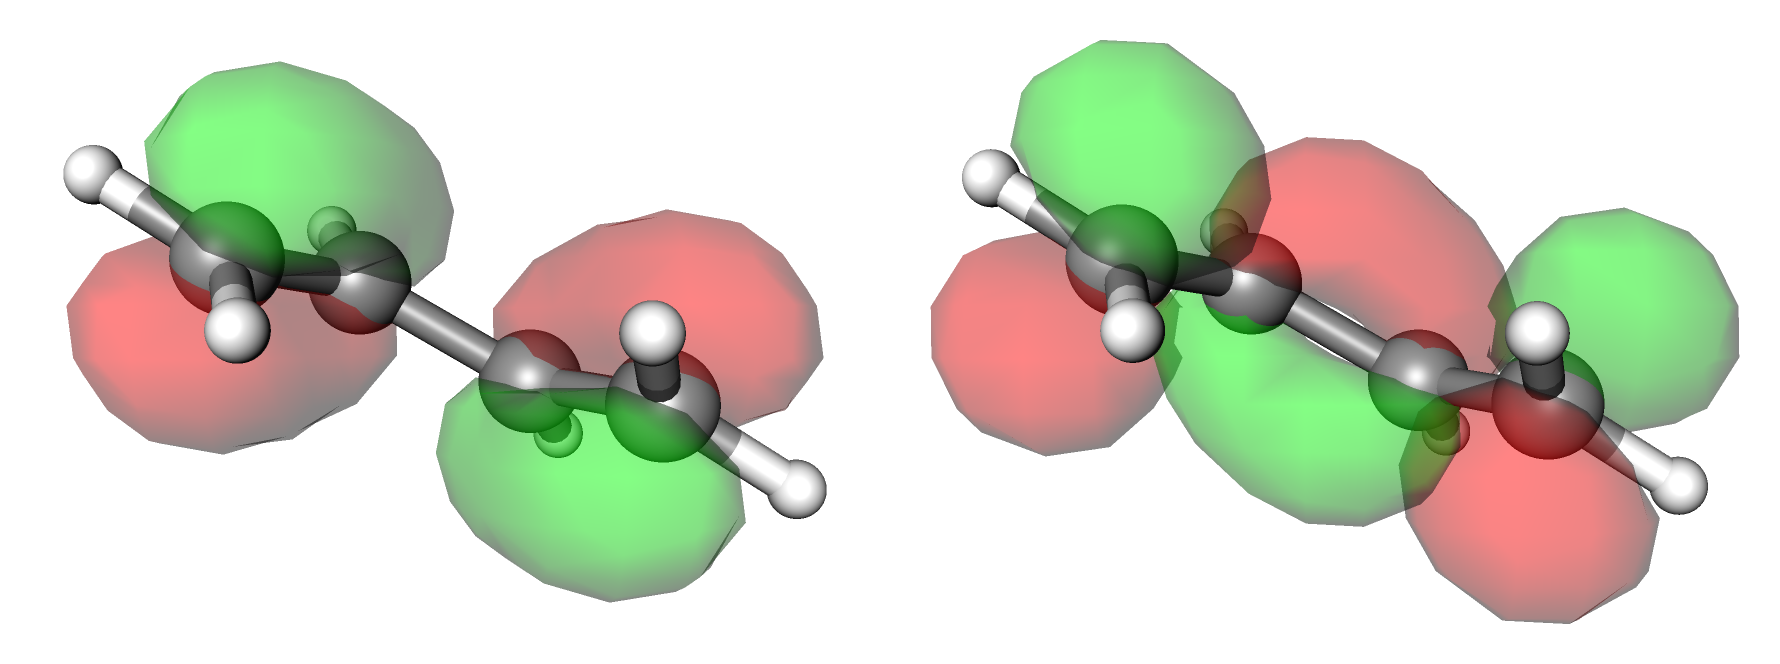
\includegraphics[width=0.9\linewidth]{density-views/homo-lumo-scis.ecce-9.5.3-dev.png}
	\caption{The HOMO (left, $\psi_2$) and the LUMO (right, $\psi_3$) of gauche butadiene, computed in the \menu{MOs} panel and seen from the same direction, onto the carbon chain with the molecule tilted about \ang{25} from face-on; the two colours are the two signs of the orbital. In the HOMO each half of the molecule, a terminal and a central carbon, carries one lobe of the same sign, and the sign changes across the central C2--C3 bond: there is a node between C2 and C3. In the LUMO the sign changes across each terminal bond, C1--C2 and C3--C4, and the two central carbons share one lobe across C2--C3.}
	\label{fig:dv-homo-lumo}
\end{figure}

The two possible gaps are almost the same: \SI{6.54}{eV} from the HOMO of butadiene to the LUMO of ethene, and \SI{6.55}{eV} from the HOMO of ethene to the LUMO of butadiene. For the parent reaction, neither direction of electron flow is preferred, and both interactions together make the reaction go. Substituents change this: an electron-donating group on the diene raises its HOMO and an electron-withdrawing group on the dienophile lowers its LUMO, which narrows the first gap and is why such pairs react much faster. So the answer to the question we started with is that the reaction is controlled by orbital overlap, not by the charges.

\XXX[figure: ethene HOMO and LUMO seen from the side (retake once ECCE lights a turned view from the camera); figure: NPA charges on the atoms]

\section{Coupling with other codes}
% What feeds this calculation (a cheaper screen, a structure from another code)
% and what it feeds (refinement, a property from the code best at it); which
% hand-off is made (usually by hand: a new calculation from this one's
% structure or orbitals in another code); a workflow only where it pays.
Natural charges computed by ECCE come from the orbitals that ECCE stores for every code, so a charge from an ORCA calculation and one from a Gaussian or ECCE-QM calculation are defined the same way, and a structure handed from one code to another keeps a comparable set of charges.

\chapter{Molecular orbital diagrams from a calculation}
\label{ch:mo-analysis}
\index{MO diagram}
\index{Molecular orbitals}
\index{Orbital symmetry}
\index{Bond order}
\eccexample{Examples > Inorganic Chemistry}
\helppage{mo-diagram}
\XXX[ chapter to be written]

\section{Background}

\section{What ECCE shows}

\section{Procedure}

\section{Results}



\part{Spectroscopy and spectrometry}
% Part overview, set before the part's first chapter.
\checkedwith{9.5.3-dev}{a9b2d49c8}

A spectrum is often the only direct evidence we have of a molecule, and calculations are used in spectroscopy for two reasons that pull in slightly different directions: to assign a measured spectrum, which means knowing which band belongs to which motion or transition, and to predict a spectrum that has not been measured, which means knowing how far to trust the calculated positions and intensities. The chapters of this part cover the spectra that ECCE reads from the codes and draws, and in each case they show both how to get the spectrum and what it can be compared with.

Vibrational spectra come from a frequency calculation, the same calculation that supplies the thermochemistry of Chapter~\ref{ch:thermochemistry}. ECCE draws the IR and, where the code computes activities, the Raman spectrum, animates each normal mode, and labels it with its symmetry and with how much of each internal coordinate it contains, so that a band can be called a C=O stretch because the calculation says so rather than because it sits where C=O stretches usually sit (Chapter~\ref{ch:vibrations}). A calculated spectrum is not a measured one, since harmonic frequencies are systematically too high and the intensities belong to an isolated molecule, and Chapter~\ref{ch:ir-experiment} shows how to put a measured spectrum next to the calculated one, scale the frequencies and match the bands.

Electronic spectra need excited states. ECCE reads the TD-DFT and CIS excitation energies, oscillator strengths and symmetries that ORCA and Gaussian~16 print, together with the orbital transitions that make up each state, and draws them as a UV--vis spectrum. Chapter~\ref{ch:excited-states} uses this to connect a colour to the orbitals involved, and is also explicit about where TD-DFT with common functionals goes wrong.

Magnetic resonance is the other main source of structural evidence. For NMR, ECCE reads the shielding tensors from Gaussian~16 and ORCA and turns the isotropic shieldings into a spectrum once a reference shielding is given, which is the step that makes a calculated shielding comparable with a measured chemical shift (Chapter~\ref{ch:nmr}). For open-shell molecules, ORCA's EPR g-tensors and hyperfine couplings are read in the same way (Chapter~\ref{ch:epr}).

The coupling between codes matters here as much as anywhere. A spectrum is only as good as the structure it is computed for, and the usual route is to find the conformers first (Chapter~\ref{ch:crest}), optimise the relevant ones, compute the spectrum of each and weight them by their Boltzmann populations, rather than computing the spectrum of the one structure that happened to be drawn.

\chapter{IR and Raman spectra and mode symmetry}
\label{ch:vibrations}
\index{IR spectrum}
\index{Raman spectrum}
\index{Normal modes}
\index{Mode symmetry}
\index{Scaling factors}
\eccexample{Examples > Spectroscopy}
\helppage{mode-composition}
\helppage{match-bands}
\helppage{displacement}
\XXX[ chapter to be written]

\section{Background}

\section{What ECCE shows}

\section{Procedure}

\section{Results}

\section{Coupling with other codes}
% What feeds this calculation (a cheaper screen, a structure from another code)
% and what it feeds (refinement, a property from the code best at it); which
% steps a workflow or recipe automates and which are a manual hand-off.


\chapter{Comparing spectra with experiment}
\label{ch:ir-experiment}
\index{Experimental spectrum}
\index{Difference spectrum}
\index{Scaling factors}
\eccexample{Examples > Spectroscopy > Sulfate coordination}
\helppage{ir-spectrum-difference-experiment}
\XXX[ chapter to be written]

\section{Background}

\section{What ECCE shows}

\section{Procedure}

\section{Results}


\chapter{Electronic excitations}
\label{ch:excited-states}
\index{TD-DFT}
\index{UV-vis}
\index{Excited states}
\eccexample{Examples > Spectroscopy}

\XXX[ chapter to be written]

\section{Background}

\section{What ECCE shows}

\section{Procedure}

\section{Results}


\chapter{NMR shielding and chemical shifts}
\label{ch:nmr}
\index{NMR}
\index{Chemical shift}
\index{Shielding tensor}
\index{GIAO}


\XXX[ chapter to be written]

\section{Background}

\section{What ECCE shows}

\section{Procedure}

\section{Results}

\section{Coupling with other codes}
% What feeds this calculation (a cheaper screen, a structure from another code)
% and what it feeds (refinement, a property from the code best at it); which
% hand-off is made (usually by hand: a new calculation from this one's
% structure or orbitals in another code); a workflow only where it pays.

\XXX[ECCE today: per-atom shielding tensors (Gaussian 16, ORCA, NWChem), no spectrum yet (issue 384).]

\chapter{EPR parameters: g-tensors and hyperfine couplings}
\label{ch:epr}
\index{EPR}
\index{g-tensor}
\index{Hyperfine coupling}
\index{Spin density}


\XXX[ chapter to be written]

\section{Background}

\section{What ECCE shows}

\section{Procedure}

\section{Results}

\section{Coupling with other codes}
% What feeds this calculation (a cheaper screen, a structure from another code)
% and what it feeds (refinement, a property from the code best at it); which
% hand-off is made (usually by hand: a new calculation from this one's
% structure or orbitals in another code); a workflow only where it pays.

\XXX[ECCE today: g-tensors and hyperfine couplings are not read yet (ORCA, issue 820); spin densities are.]


\part{Organic chemistry}
% Part overview, set before the part's first chapter.
\checkedwith{9.5.3-dev}{a9b2d49c8}

Most computational work in organic chemistry asks one of a handful of questions: what a molecule looks like, which of its shapes it actually adopts, how stable it is relative to an isomer or a product, how fast it reacts and by which path, and what its spectra should look like. This part, together with the reaction and spectroscopy chapters it points to, shows how each of these is done in ECCE and how the answer from one code is handed to the next.

The first question is about bonding rather than energies. When we draw ethene with two sp$^2$ carbons and a $\pi$ bond, we are using a localised picture that the canonical orbitals of a calculation do not show directly. ECCE-QM can transform the occupied orbitals into localised ones and label each bond with its hybrid composition, so that the textbook picture can be checked against the calculation and its limits seen; Chapter~\ref{ch:localised-bonds} does this for ethane, ethene and ethyne.

Conformers come next, because nearly every property of a flexible molecule is an average over the shapes it adopts at room temperature, and a structure optimised from one drawn geometry is only one of them, and not necessarily the lowest. In ECCE the route is CREST, which searches conformational space with the semi-empirical GFN2-xTB method and returns an ensemble with Boltzmann weights (Chapter~\ref{ch:crest}). The same program finds the likely protonation sites and tautomers of a molecule (Chapter~\ref{ch:protonation}), which matters whenever an acid--base equilibrium or a hydrogen shift decides what is actually present in solution.

These searches are affordable only because xTB is cheap, and Chapter~\ref{ch:xtb} shows what xTB is good for on its own: geometries, a first look at reaction energies, and screening a set of molecules before anything expensive is run. The pattern that runs through the rest of the book starts here. A cheap method ranks many candidates, a density functional calculation in ORCA, Gaussian~16 or ECCE-QM refines the few that matter, and the hand-off between them is made in ECCE, usually by hand with \menu{New from This}, or with a workflow when the chain is long enough to be worth automating (Chapters~\ref{ch:coupling} and \ref{ch:workflows}). Note that the energies of the two levels are never compared with each other; the cheap method only decides which structures go on.

Reactions are treated in the Physical chemistry part, since the methods are not specific to organic chemistry. Reaction and activation energies, enthalpies and Gibbs energies are covered in Chapter~\ref{ch:thermochemistry}; finding a transition state, confirming it by its single imaginary frequency and following the reaction path down to reactants and products with an IRC in Chapter~\ref{ch:reaction-rates}; and rotational barriers and other relaxed scans in Chapter~\ref{ch:scans}. The organic examples that ship with ECCE, substitution against elimination for fluoride and chloroethane, and keto--enol tautomerism with and without a water molecule as a proton relay, were made for these chapters.

Spectra are where the calculations meet experiment. IR and Raman spectra, with the symmetry and composition of each mode, are in Chapter~\ref{ch:vibrations}, the comparison of a calculated spectrum with a measured one in Chapter~\ref{ch:ir-experiment}, UV--vis spectra in Chapter~\ref{ch:excited-states}, and NMR chemical shifts in Chapter~\ref{ch:nmr}. Finally, when the question is about a series of molecules rather than one, the descriptors of Chapter~\ref{ch:qsar} turn a folder of calculations into a table that can be fitted against a measured activity, and Chapter~\ref{ch:docking} shows how a molecule optimised here is docked into a protein.

\chapter{Localised bonds: ethane, ethene and ethyne}
\label{ch:localised-bonds}
\index{Localised orbitals}
\index{Hybridisation}
\index{Bond order}
\index{s character}
\index{Pipek-Mezey localisation}
\index{Ethane}\index{Ethene}\index{Ethyne}
\checkedwith{9.5.3-dev}{7e2077af7}
\eccexample{Examples > Organic Chemistry > Bonding in hydrocarbons}
\helppage{localised-orbitals}

Organic chemistry describes ethane, ethene and ethyne with one picture each: four sp$^3$ hybrids on each carbon of ethane, three sp$^2$ hybrids and a p orbital in ethene, two sp hybrids and two p orbitals in ethyne. The orbitals a quantum chemistry program gives are spread over the whole molecule and look nothing like this. ECCE-QM, the program built into ECCE, can turn them into localised orbitals, one for each bond and lone pair, and label each with the hybrid it uses on each atom. This chapter puts the three molecules side by side and asks how well the hybrid picture holds: which bonds ECCE finds, how much s character the carbon hybrids have, and how that goes with the bond lengths, the angles and the stretching frequencies.

\section*{This requires}
Nothing beyond ECCE: the three calculations are in the Organic Chemistry example set. Localised orbitals and their hybrid labels are available only for ECCE-QM calculations.

\section{Background}
A localised orbital describes the same electrons as the orbitals of the calculation, divided up differently. The occupied orbitals are mixed among themselves until each one sits on as few atoms as possible, and what comes out is, for an ordinary closed-shell molecule, one orbital per core, bond and lone pair. The total electron density and the energy do not change; only the bookkeeping does. ECCE-QM uses the criterion of Pipek and Mezey \cite{pipek1989}, which makes each orbital's charge sit on as few atoms as possible. In a planar molecule such as ethene this criterion keeps the $\sigma$ and the $\pi$ bond apart, so the localised orbitals come out in the form organic chemistry draws.

For each localised bond orbital ECCE works out how much of it is s and how much p on each of the two atoms, and writes the ratio as a hybrid label. \texttt{sp3.6} means 3.6 times as much p as s, so the hybrid is $1/(1+3.6) = 22\,\%$ s. The ideal hybrids of the textbook are sp$^3$ (25\,\% s), sp$^2$ (33\,\%) and sp (50\,\%). A hydrogen contributes only its s orbital, written \texttt{s}, and a $\pi$ bond gets no label because it is made of p orbitals across the bond. The labels are worked out from the orbitals and rounded to one decimal, so they describe the bond; they are not a measured quantity.
\index{Hybridisation!s character}

\section{The calculations}
The topic \menu{Bonding in hydrocarbons} has three ECCE-QM calculations made for this comparison, \emph{ethane}, \emph{ethene} and \emph{ethyne}. Each is a geometry optimisation followed by frequencies with B3LYP \cite{becke1993} and the 6-31G* basis \cite{hariharan1973}, with \menu{Localised orbitals} ticked under \menu{Runtype Details}. All three use the same method, so their bond lengths and hybrids can be compared directly.

\section{Procedure}
\begin{enumerate}
	\item In the Organizer, choose \menu{File > Open Example Calculations}, pick \menu{Organic Chemistry} and click \menu{OK}.
	\item In \menu{Examples > Bonding in hydrocarbons}, open \emph{ethane} in the Viewer and choose \menu{Properties > MOs}.
	\item In the box next to \menu{Compute}, choose \menu{Localised MO} instead of \menu{MO}. The table now lists the localised orbitals, with the columns \menu{Bond type}, \menu{Atoms} and \menu{Hybrids} (figure~\ref{fig:lb-table}).
	\item Select the row with \menu{$\sigma$} and \menu{C1-C2} and click \menu{Compute} to draw the orbital; then one of the $\sigma$ C1--H rows.
	\item With \menu{Measure}, measure C1--C2, C1--H3, the angle H3--C1--H4 and the angle H3--C1--C2.
	\item Open \menu{Properties > Vibrational spectra > Vibrational Frequencies} and look at the C--H stretches near 3000~cm$^{-1}$ and above.
	\item Repeat for \emph{ethene} and \emph{ethyne}, and draw their $\pi$ orbitals too.
\end{enumerate}
\index{Localised orbitals!showing}\index{MOs panel!Localised MO}\index{Measure}

\begin{figure}[htbp]
	\centering
	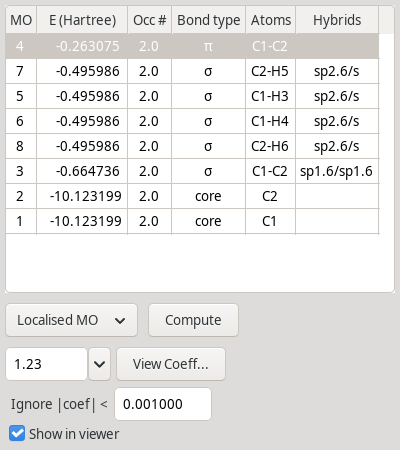
\includegraphics[width=0.5\linewidth]{localised-bonds/loctable-ethene.ecce-9.5.3-dev.png}
	\caption{The localised orbitals of ethene in the \menu{MOs} panel (\menu{Localised MO}). Each row names one core orbital, bond or lone pair, the atoms it belongs to and, for a $\sigma$ bond, the hybrid on each atom.}
	\label{fig:lb-table}
\end{figure}

\section{The bonds ECCE finds}
The localised orbitals come out exactly as the Lewis structures are drawn (table~\ref{tab:lb-orbitals}). Each molecule has two carbon core orbitals and one $\sigma$ orbital for every C--H bond. The C--C bond is one $\sigma$ orbital in ethane, a $\sigma$ and a $\pi$ orbital in ethene, and a $\sigma$ and two $\pi$ orbitals in ethyne. Counting the orbitals between the two carbons gives the bond order, 1, 2 and 3.

\begin{table}[htbp]
	\centering
	\caption{The occupied localised orbitals of the three molecules as the \menu{MOs} panel lists them (B3LYP/6-31G*), with its columns \menu{Bond type}, \menu{Atoms}, \menu{Hybrids} and \menu{E (Hartree)}; orbitals of the same kind are counted together. Every orbital holds two electrons.}
	\label{tab:lb-orbitals}
	\begin{tabular}{lllllr}
		\toprule
		Molecule & Bond type & Atoms & Hybrids & Number & $E$ (hartree) \\
		\midrule
		ethane & core & C1, C2 & & 2 & $-10.125$ \\
		       & $\sigma$ & C1-C2 & sp2.7/sp2.7 & 1 & $-0.517$ \\
		       & $\sigma$ & C-H & sp3.6/s & 6 & $-0.466$ \\
		\midrule
		ethene & core & C1, C2 & & 2 & $-10.123$ \\
		       & $\sigma$ & C1-C2 & sp1.6/sp1.6 & 1 & $-0.665$ \\
		       & $\pi$ & C1-C2 & & 1 & $-0.263$ \\
		       & $\sigma$ & C-H & sp2.6/s & 4 & $-0.496$ \\
		\midrule
		ethyne & core & C1, C2 & & 2 & $-10.104$ \\
		       & $\sigma$ & C1-C2 & sp0.8/sp0.8 & 1 & $-0.807$ \\
		       & $\pi$ & C1-C2 & & 2 & $-0.278$ \\
		       & $\sigma$ & C-H & sp1.4/s & 2 & $-0.568$ \\
		\bottomrule
	\end{tabular}
\end{table}

The pictures (figure~\ref{fig:lb-orbitals}) show what the labels mean. The C--H orbital is a single lobe between the carbon and the hydrogen, with a small tail on the far side of the carbon. The C--C $\sigma$ orbital is symmetric about the C--C axis. The $\pi$ orbital of ethene has two lobes, above and below the plane of the atoms, with a node in that plane. In ethyne the two $\pi$ orbitals are the same shape at right angles to each other, and together they make a cylinder of density around the C--C axis.

\begin{figure}[htbp]
	\centering
	\begin{tabular}{@{}ccc@{}}
		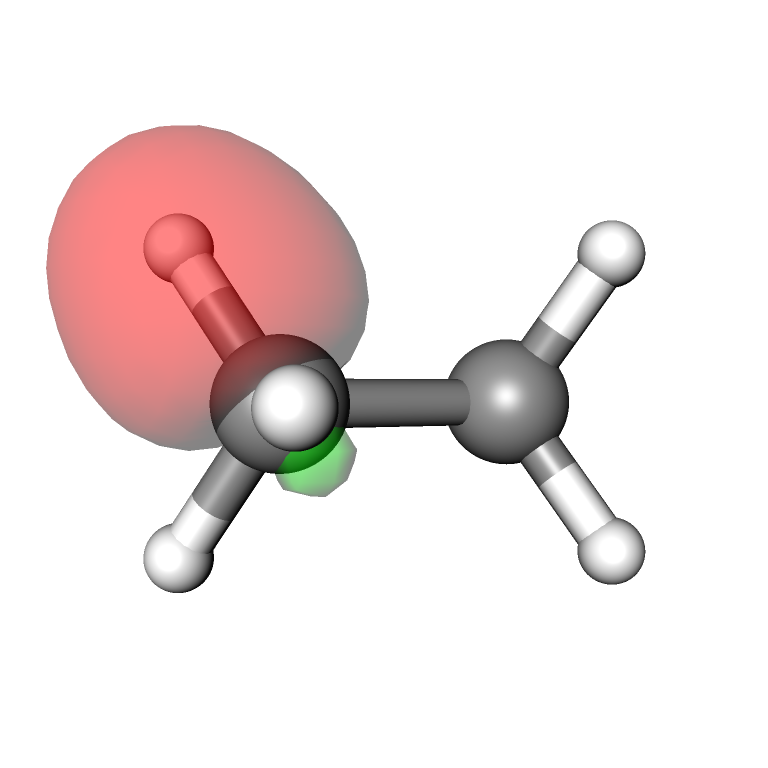
\includegraphics[width=0.31\linewidth]{localised-bonds/ethane-ch-sigma.ecce-9.5.3-dev.png} &
		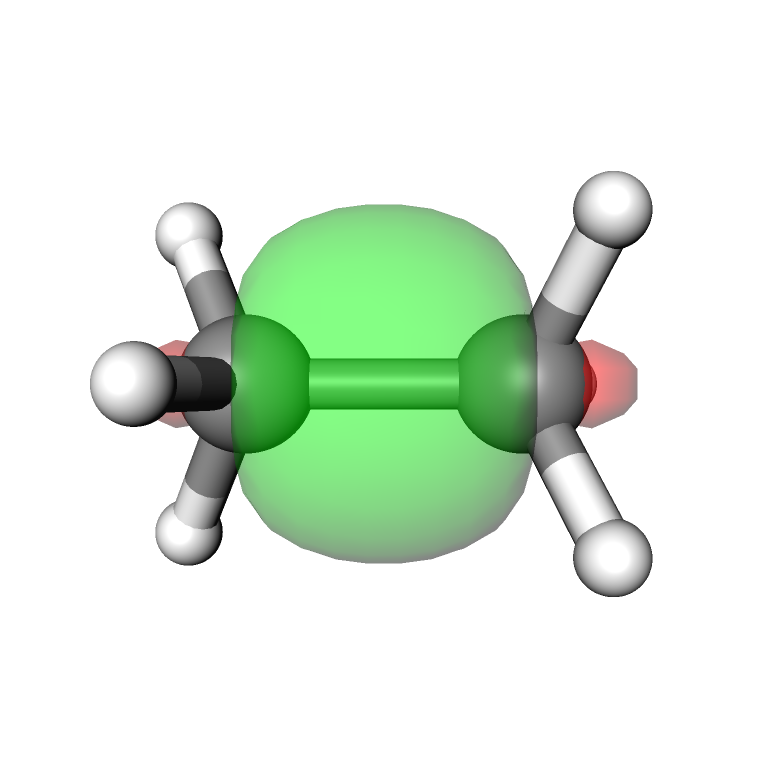
\includegraphics[width=0.31\linewidth]{localised-bonds/ethane-cc-sigma.ecce-9.5.3-dev.png} & \\
		\small ethane, $\sigma$ C--H & \small ethane, $\sigma$ C--C & \\[4pt]
		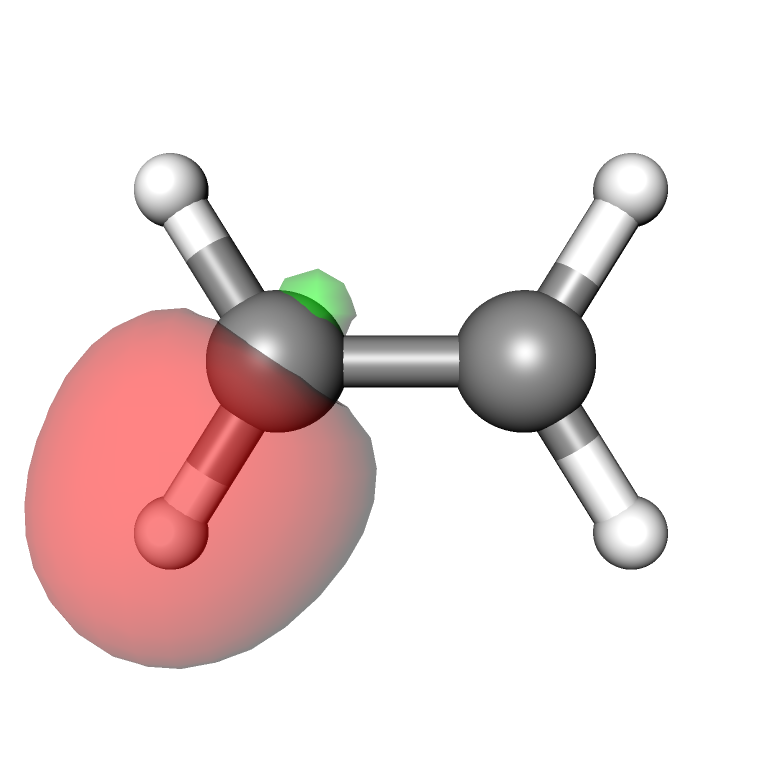
\includegraphics[width=0.31\linewidth]{localised-bonds/ethene-ch-sigma.ecce-9.5.3-dev.png} &
		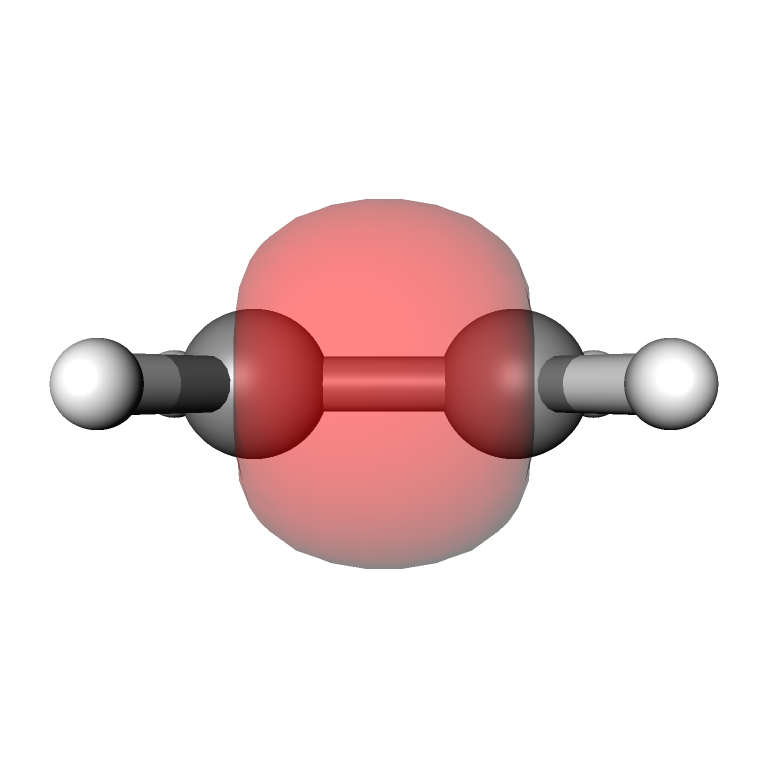
\includegraphics[width=0.31\linewidth]{localised-bonds/ethene-cc-sigma.ecce-9.5.3-dev.png} &
		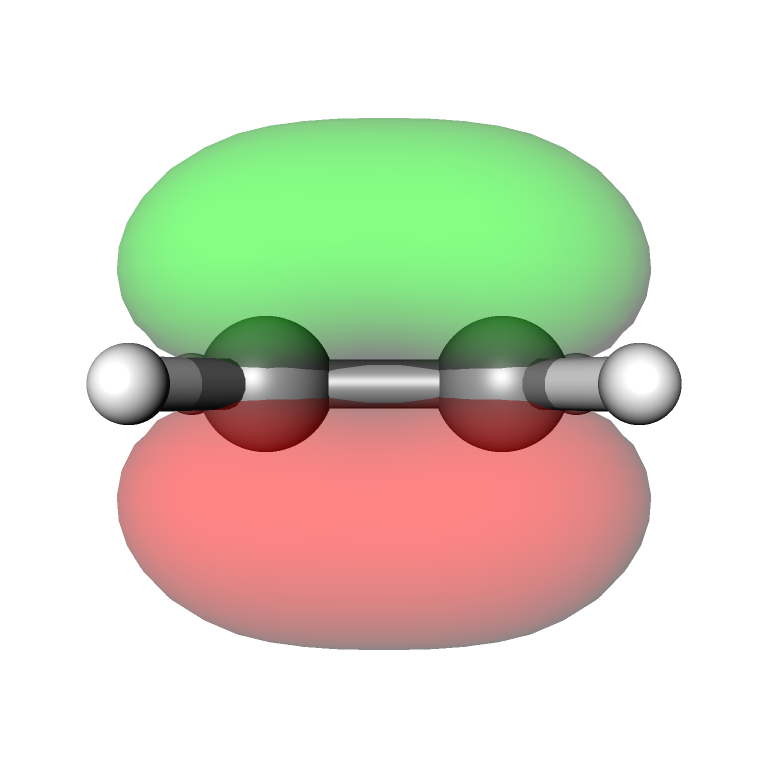
\includegraphics[width=0.31\linewidth]{localised-bonds/ethene-cc-pi.ecce-9.5.3-dev.png} \\
		\small ethene, $\sigma$ C--H & \small ethene, $\sigma$ C--C & \small ethene, $\pi$ C--C \\[4pt]
		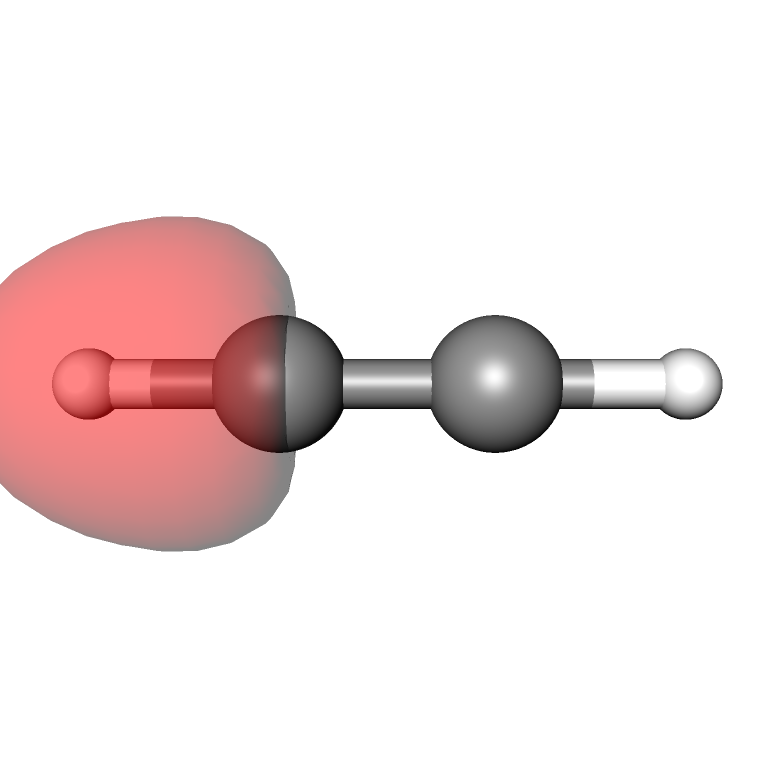
\includegraphics[width=0.31\linewidth]{localised-bonds/ethyne-ch-sigma.ecce-9.5.3-dev.png} &
		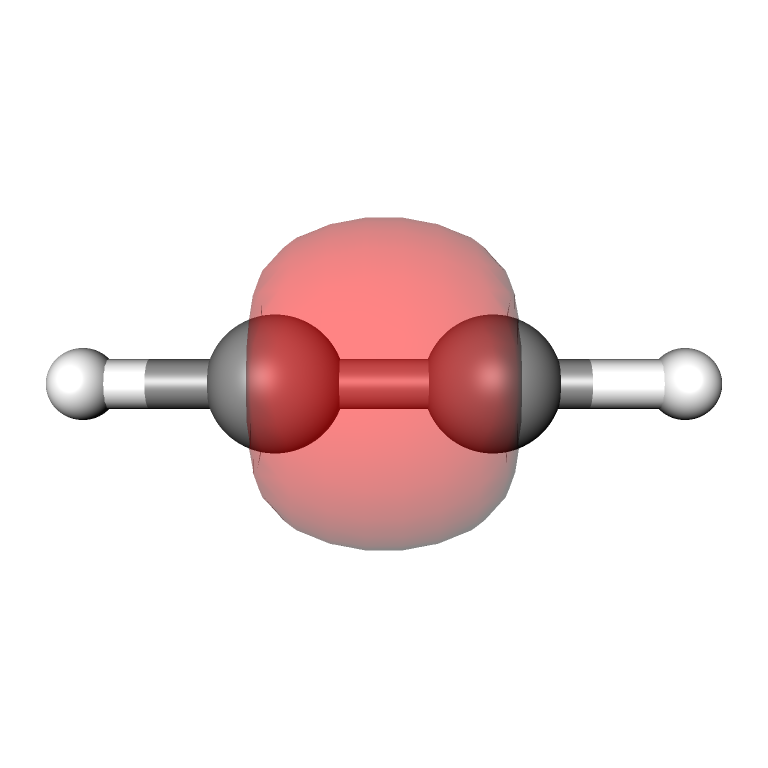
\includegraphics[width=0.31\linewidth]{localised-bonds/ethyne-cc-sigma.ecce-9.5.3-dev.png} &
		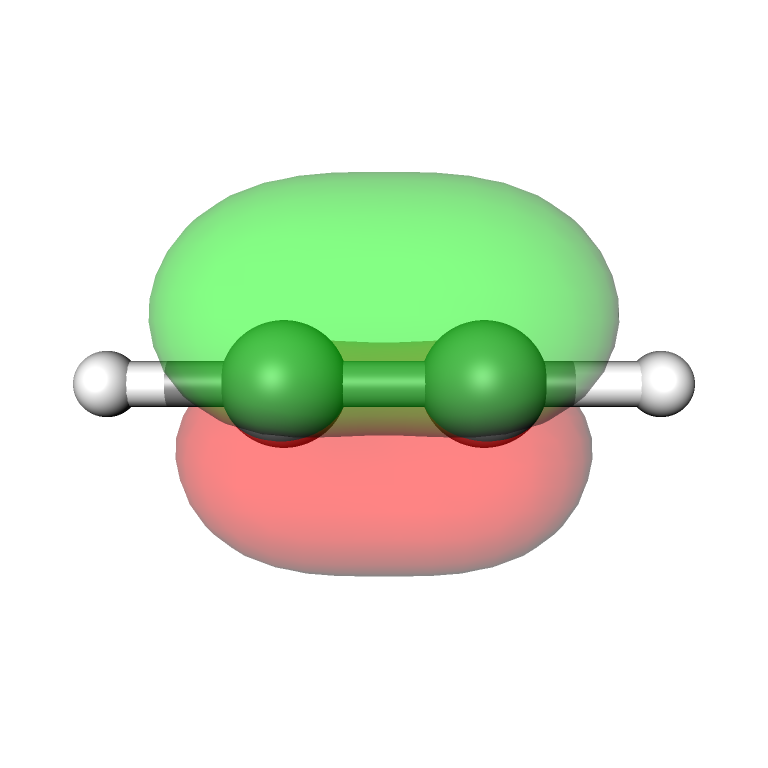
\includegraphics[width=0.31\linewidth]{localised-bonds/ethyne-cc-pi1.ecce-9.5.3-dev.png} \\
		\small ethyne, $\sigma$ C--H & \small ethyne, $\sigma$ C--C & \small ethyne, one of the two $\pi$ \\
	\end{tabular}
	\caption{Localised orbitals of ethane, ethene and ethyne drawn by the \menu{MOs} panel (\menu{Localised MO}, default isovalue; the two colours are the two signs of the orbital). Each molecule is shown with its C--C axis across the page.}
	\label{fig:lb-orbitals}
\end{figure}

\section{Hybrids and s character}
Table~\ref{tab:lb-trends} collects the hybrid labels with the geometry and the stretching frequencies. On carbon, the s character of both kinds of $\sigma$ bond rises from ethane to ethene to ethyne: in the C--H bond from 22 to 28 to 42\,\%, in the C--C bond from 27 to 38 to 56\,\%. The trend is the one the textbook names, sp$^3$, sp$^2$, sp, but the numbers are not the ideal 25, 33 and 50\,\%. In each molecule the carbon puts more s character into the bond to the other carbon than into its bonds to hydrogen, so that even in ethane the four bonds of a carbon are not four identical sp$^3$ hybrids. In ethene and ethyne the $\pi$ bonds take p orbitals only, which leaves the s orbital of carbon to the $\sigma$ bonds; that is why the $\sigma$ hybrids of the multiple bonds are so rich in s.

The hybrids explain the angles. An sp$^3$ carbon has its bonds at the tetrahedral angle, \ang{109.5}; ethane comes close, with H--C--H \ang{107.5} and H--C--C \ang{111.3}. The H--C--H angle in ethene, \ang{116.3}, is a few degrees below the \ang{120} of three equal sp$^2$ hybrids, and H--C--C opens to \ang{121.9}, as the carbon with more s character towards the other carbon would make it. Ethyne is linear.
\index{Bond angles!hybridisation}

\begin{table}[htbp]
	\centering
	\caption{Hybrids, geometry and stretching frequencies of the three molecules (ECCE-QM, B3LYP/6-31G*, optimised geometries). Hybrid labels from the \menu{MOs} panel; s character on carbon is $1/(1+n)$ for a label sp$n$. Lengths and angles from the optimised structures, frequencies from \menu{Vibrational Frequencies} (harmonic, not scaled).}
	\label{tab:lb-trends}
	\begin{tabular}{lrrr}
		\toprule
		 & ethane & ethene & ethyne \\
		\midrule
		C--C bond order & 1 & 2 & 3 \\
		C--C $\sigma$ hybrid on C & sp2.7 & sp1.6 & sp0.8 \\
		\quad s character & 27\,\% & 38\,\% & 56\,\% \\
		C--H $\sigma$ hybrid on C & sp3.6 & sp2.6 & sp1.4 \\
		\quad s character & 22\,\% & 28\,\% & 42\,\% \\
		\midrule
		C--C (\AA) & 1.531 & 1.332 & 1.205 \\
		C--H (\AA) & 1.097 & 1.088 & 1.067 \\
		H--C--H & \ang{107.5} & \ang{116.3} & -- \\
		H--C--C & \ang{111.3} & \ang{121.9} & \ang{180.0} \\
		\midrule
		C--C stretch (cm$^{-1}$) & 1009 & 1719 & 2086 \\
		C--H stretches (cm$^{-1}$) & 3045--3120 & 3149--3245 & 3440, 3540 \\
		\bottomrule
	\end{tabular}
\end{table}

\section{Bond lengths and stretching frequencies}
The C--C bond shortens from \SI{1.531}{\angstrom} in ethane to \SI{1.332}{\angstrom} in ethene and \SI{1.205}{\angstrom} in ethyne, and its stretch moves up from 1009 to 1719 and 2086~cm$^{-1}$ (all three are the totally symmetric C--C stretch, which is not IR active in these molecules). Both follow the bond order, the number of localised orbitals between the carbons.

The C--H bond changes much less, but in the same direction: \SI{1.097}{\angstrom}, \SI{1.088}{\angstrom} and \SI{1.067}{\angstrom}. Here the bond order is one in all three molecules, and what changes is the carbon hybrid. A hybrid with more s character holds its electrons closer to the carbon nucleus, so the bond is shorter and stiffer, and the C--H stretches rise from 3045--3120~cm$^{-1}$ in ethane to 3149--3245 in ethene and 3440 and 3540~cm$^{-1}$ in ethyne. The energies of the localised C--H orbitals in table~\ref{tab:lb-orbitals} fall in the same order, from $-0.466$ to $-0.496$ to $-0.568$~hartree: the electrons of the C--H bond are held more tightly as the s character rises.
\index{Bond length!s character}\index{Infrared spectrum!C--H stretch}

\section{What the labels do not say}
The s shares of the four $\sigma$ bonds of a carbon add up to 0.92 in ethane ($3 \times 0.217 + 0.270$), 0.94 in ethene and 0.97 in ethyne, close to one 2s orbital but not exactly one. Each label is worked out from its own orbital, leaves out the small contribution of the d functions of the basis set and is rounded to one decimal. The labels should be read as a trend between molecules and between bonds, with an uncertainty of a few per cent, rather than as exact compositions.

\section{In class}
Start from the Lewis structures and ask what each line stands for; the \menu{Localised MO} table answers with one orbital per line, and the $\pi$ orbitals of ethene and ethyne are the second and third lines of the multiple bonds. The table of hybrids is then a test of the sp$^3$/sp$^2$/sp picture: the order is right, the numbers are not the ideal ones, and the difference between the C--C and the C--H hybrids of the same carbon is the point where the simple picture needs refining. The C--H bond length and the C--H stretch tie the hybrid to things that can be measured; the high C--H stretch of ethyne is the band by which a terminal alkyne is recognised in an infrared spectrum.

\section{History}
Pauling \cite{pauling1931} and Slater \cite{slater1931} introduced hybrid orbitals in 1931 to explain why carbon forms four equivalent bonds at the tetrahedral angle when its valence orbitals are one 2s and three 2p orbitals. The first systematic ways to turn the delocalised orbitals of a calculation into localised ones came three decades later: Foster and Boys made each orbital as compact in space as possible \cite{foster1960}, and Edmiston and Ruedenberg maximised the repulsion of the electrons within each orbital \cite{edmiston1963}. Both criteria give a double bond as two equivalent bent bonds rather than a $\sigma$ and a $\pi$ bond. Pipek and Mezey's criterion, which counts how many atoms an orbital's charge is spread over \cite{pipek1989}, keeps $\sigma$ and $\pi$ apart and gives the description used in this chapter.
\index{Pauling, Linus}\index{Slater, John C.}\index{Boys, S. Francis}\index{Edmiston, Clyde}\index{Ruedenberg, Klaus}\index{Pipek, J\'anos}\index{Mezey, Paul G.}

\chapter{Conformer searches with CREST: from one structure to a refined ensemble}
\chaptermark{Conformer searches with CREST}
\label{ch:crest}
\index{CREST}
\index{Conformer search}
\index{Boltzmann weights}
\index{Coupled codes}
\checkedwith{9.5.3-dev}{d26701ae0}
\helppage{crest}

A molecule that can rotate about its single bonds has no single structure, and the structure we draw is one point on a surface with many minima. Whether it matters which minimum we compute depends on the question. For a rigid aromatic ring it does not, whereas for a flexible chain with a donor and an acceptor for a hydrogen bond it decides the energy, the dipole moment, the NMR couplings and, further down the road, the binding to a protein. In this chapter we search for the minima with CREST, read the resulting ensemble in ECCE, and decide which of its members deserve a more expensive calculation. The example is 2-methoxyethanol, \chem{CH3OCH2CH2OH}, a molecule small enough for the search to take three minutes and flexible enough to show what an ensemble looks like.

\section{Background}
\index{Conformers!when they matter}\index{Intramolecular hydrogen bonds}\index{Ring puckers}\index{Rotamers}

A conformer is a minimum of the energy surface that differs from the others by rotation about single bonds or, in a ring, by a change of pucker. Conformers matter whenever the energy differences between them are comparable to $RT$, which is $0.59$~kcal/mol at 298~K, since the measured property is then an average over several structures. The cases an organic chemist meets most often are the chair and twist-boat forms of rings and the axial or equatorial position of a substituent, the rotamers of an alkyl chain, the \emph{cis} and \emph{trans} forms of an amide or ester, and any molecule in which a donor and an acceptor can reach each other, so that the internal hydrogen bond competes with the extended chain.

2-Methoxyethanol has two rotations that set this competition. About the central C--C bond the two oxygen atoms are either \emph{gauche}, which lets the hydroxyl hydrogen reach the ether oxygen in a five-membered ring, or \emph{anti}, which keeps them apart. The C--O bonds add further rotamers of the hydroxyl and the methyl group. A person looking at a drawing would guess the \emph{gauche} form with the hydrogen bond, and the search tells us how much of the ensemble that guess accounts for.

CREST \cite{pracht2020} finds the minima by running short metadynamics trajectories from the input structure, which push the molecule over rotational barriers, optimising the snapshots and sorting out duplicates. Since the trajectories and the optimisations use a tight-binding method, GFN2-xTB \cite{bannwarth2019} or the force field GFN-FF \cite{spicher2020}, the search takes minutes for a molecule of this size and hours for a drug-sized one, where a density functional calculation on every starting structure would not be possible. The price is that the energies of such methods order conformers only roughly, and the chapter returns to that when we choose what goes on to a better level.
\index{GFN2-xTB}\index{GFN-FF}\index{Metadynamics}

\section{What ECCE shows}
\index{CREST!run types}\index{Run types!CREST}

The \menu{CREST} button in the code bar makes a calculation with this code. CREST runs \cmd{xtb} itself, so both programs are registered for the machine in \menu{Register Machines}, and the xTB path of the machine is the one CREST uses. Four run types are offered. \menu{Conformer Search} is the one of this chapter. \menu{Protonation Sites} adds a proton at every basic site of the molecule and returns the protonated structures, lowest first, and \menu{Tautomers} moves protons between the sites; both work with GFN2-xTB only and have an energy window of 30~kcal/mol, and Chapter~\ref{ch:protonation} puts them to use. \menu{Solvation Shell} grows a cluster of solvent molecules around the solute, the subject of Chapter~\ref{ch:pom-solvation}.
\index{CREST!Protonation Sites}\index{CREST!Tautomers}\index{CREST!Solvation Shell}

The \menu{Theory} of a conformer search is \menu{GFN2-xTB}, the default; \menu{GFN-FF}, which is much faster and suits a first look at a large floppy system; or \menu{GFN2//GFN-FF}, which searches with the force field and re-optimises and ranks with GFN2-xTB. The \menu{Theory Details} offer an implicit solvent, ALPB or GBSA, and \menu{Runtype Details} the \menu{Energy window} in kcal/mol (6 by default), which sets how far above the lowest conformer a structure may lie and still be kept. Two options exist for special cases. \menu{Non-covalent complex (NCI mode)} keeps the parts of a host--guest complex together, and the two topology options (\menu{Skip the reference-topology check} and \menu{No topology check}) stop CREST from discarding structures whose bonds it reads differently from the input, which happens for ion clusters.
\index{CREST!Energy window}\index{CREST!Theory}\index{Implicit solvent!ALPB}\index{ALPB}\index{CREST!NCI mode}

CREST has to start from an optimised structure. An xTB geometry optimisation is therefore the first calculation, and the Launch of a CREST calculation warns when it does not follow one (\menu{Launch anyway} goes on).
\index{CREST!starting structure}

\section{Procedure}
\index{Tools menu!Add from SMILES...}\index{SMILES}

Everything happens in one project folder of the Organizer, so that each calculation can take its structure from the one before.
\begin{enumerate}
	\item With \menu{File > New} make an xTB calculation. In the Builder choose \menu{Tools > Add from SMILES...}, enter \texttt{COCCO}, and set the run type to Geometry with the theory GFN2-xTB. Launch it.
	\item Click the \menu{CREST} button in the code bar to make a CREST calculation, and give it the structure of the xTB result. Choose the run type \menu{Conformer Search} and the theory \menu{GFN2-xTB}, leave the \menu{Energy window} at 6~kcal/mol, and launch it with four cores in the Launcher.
	\item For the second search make a copy of the CREST calculation and set the implicit solvent in \menu{Theory Details} to ALPB, solvent water. Launch it.
	\index{CREST!Implicit Solvent}
	\item When a search is complete, open it in the Builder and choose \menu{Properties > Geometry > Conformers}. The columns can be sorted, \menu{Export .csv...} saves the table and \menu{Export .png...} the table with its pictures.
	\item To compare structures, Ctrl-click several rows. The Builder fits them onto the first one clicked, and the key below the table lists the colour of each member and its heavy-atom RMSD to that reference.
	\index{Conformers panel!Superposing members}\index{RMSD}
	\item To refine the conformers worth keeping, select their rows and choose \menu{New Calculation from Selected...}, which asks once for the code and makes one geometry optimisation for each, named after the CREST calculation with \texttt{\_conf} and the rank.
	\index{Conformers panel!New Calculation from Selected}
\end{enumerate}

We made the calculations of this chapter headless, through ECCE's own Launch with the decks that the same scripts write for the Calculation Editor, in an isolated data folder (ECCE 9.5.3-dev, \cmd{nice} level 19, four cores). The harness stores the structure and deck of each calculation and not the Calculation Editor setup, and the starting structure came from Open Babel with the same SMILES string. The Organizer and Builder steps follow the help pages and were driven through the windows only as far as opening the \menu{Conformers} panel.

\section{Results}
\index{2-Methoxyethanol}

\subsection{The ensemble}
The xTB optimisation took 40~s, the GFN2-xTB search 193~s on four cores. CREST kept 16 conformers within 6~kcal/mol, of which the first eight are in Table~\ref{tab:crest-gas} together with two measures that we read from the stored coordinates, the O--C--C--O dihedral and the distance from the hydroxyl hydrogen to the ether oxygen. Figure~\ref{fig:crest-table} shows the same list in the \menu{Conformers} panel.
\index{Boltzmann weights!Conformers panel}

\begin{table}[htb]
	\centering
	\caption{The eight lowest conformers of 2-methoxyethanol from the GFN2-xTB search in the gas phase. $\Delta E$ is relative to the lowest conformer of this search, the weight is the Boltzmann population at 298.15~K, $\tau$ the O--C--C--O dihedral and $d$ the H$\cdots$O distance from the hydroxyl hydrogen to the ether oxygen.}
	\label{tab:crest-gas}
	\begin{tabular}{rrrrr}
		\toprule
		Rank & $\Delta E$ (kcal/mol) & Weight (\%) & $\tau$ (\si{\degree}) & $d$ (\si{\angstrom}) \\
		\midrule
		1 & 0.000 & 48.9 & 63 & 2.40 \\
		2 & 0.373 & 26.0 & $-58$ & 2.35 \\
		3 & 1.118 & 7.4 & 172 & 3.87 \\
		4 & 1.499 & 3.9 & $-82$ & 3.53 \\
		5 & 1.586 & 3.4 & 178 & 3.89 \\
		6 & 1.665 & 2.9 & 169 & 3.95 \\
		7 & 1.777 & 2.4 & 45 & 2.60 \\
		8 & 2.205 & 1.2 & $-96$ & 3.11 \\
		\bottomrule
	\end{tabular}
\end{table}

\begin{figure}[htb]
	\centering
	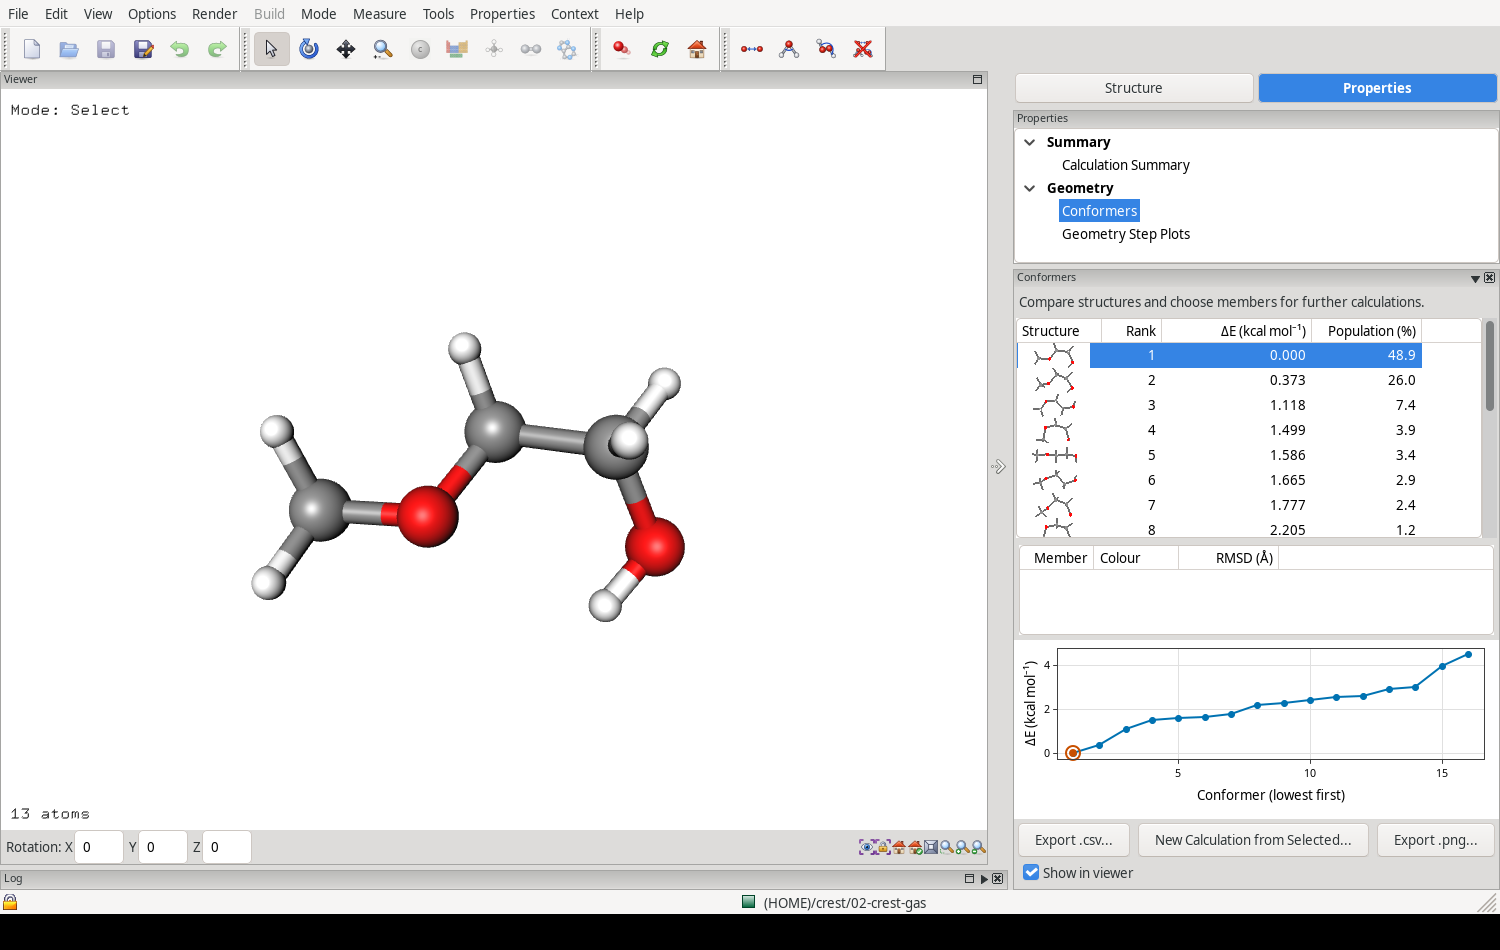
\includegraphics[width=\linewidth]{crest/conformers-gas.ecce-9.5.3-dev.png}
	\caption{The \menu{Conformers} panel for the gas-phase search on 2-methoxyethanol. The table lists rank, relative energy and population, the plot below it the energy against the rank, and the 3-D view shows the lowest conformer on a white background.}
	\label{fig:crest-table}
\end{figure}

The two lowest conformers are \emph{gauche} about the central bond, with the hydroxyl hydrogen \SI{2.40}{\angstrom} and \SI{2.35}{\angstrom} from the ether oxygen, and in the lowest the O$\cdots$O distance is \SI{2.84}{\angstrom}. They are five-membered rings closed by the hydrogen bond. Taken together with rank 7, the only other conformer with a hydrogen to oxygen distance below \SI{2.6}{\angstrom}, they carry 77~percent of the weight of the ensemble. Ranks 3, 5, 6, 11 and 12 are \emph{anti}, with the two oxygens on opposite sides, and carry 15~percent. Rank 4 is \emph{gauche} as well, but with the hydroxyl turned away, which shows that the \emph{gauche} arrangement alone does not make the bond.

The first two conformers differ by 0.37~kcal/mol, which is below what a tight-binding method resolves, so we treat them as one group and not as a ranking. Superposing ranks 1, 2 and 3 (Fig.~\ref{fig:crest-overlay}) shows what the numbers describe: the heavy-atom RMSD of rank 2 to rank 1 is \SI{0.55}{\angstrom}, since both have the same ring of five atoms and differ in the orientation of the methyl group and the hydroxyl, whereas rank 3, with the chain extended, lies \SI{0.84}{\angstrom} away.

\begin{figure}[htb]
	\centering
	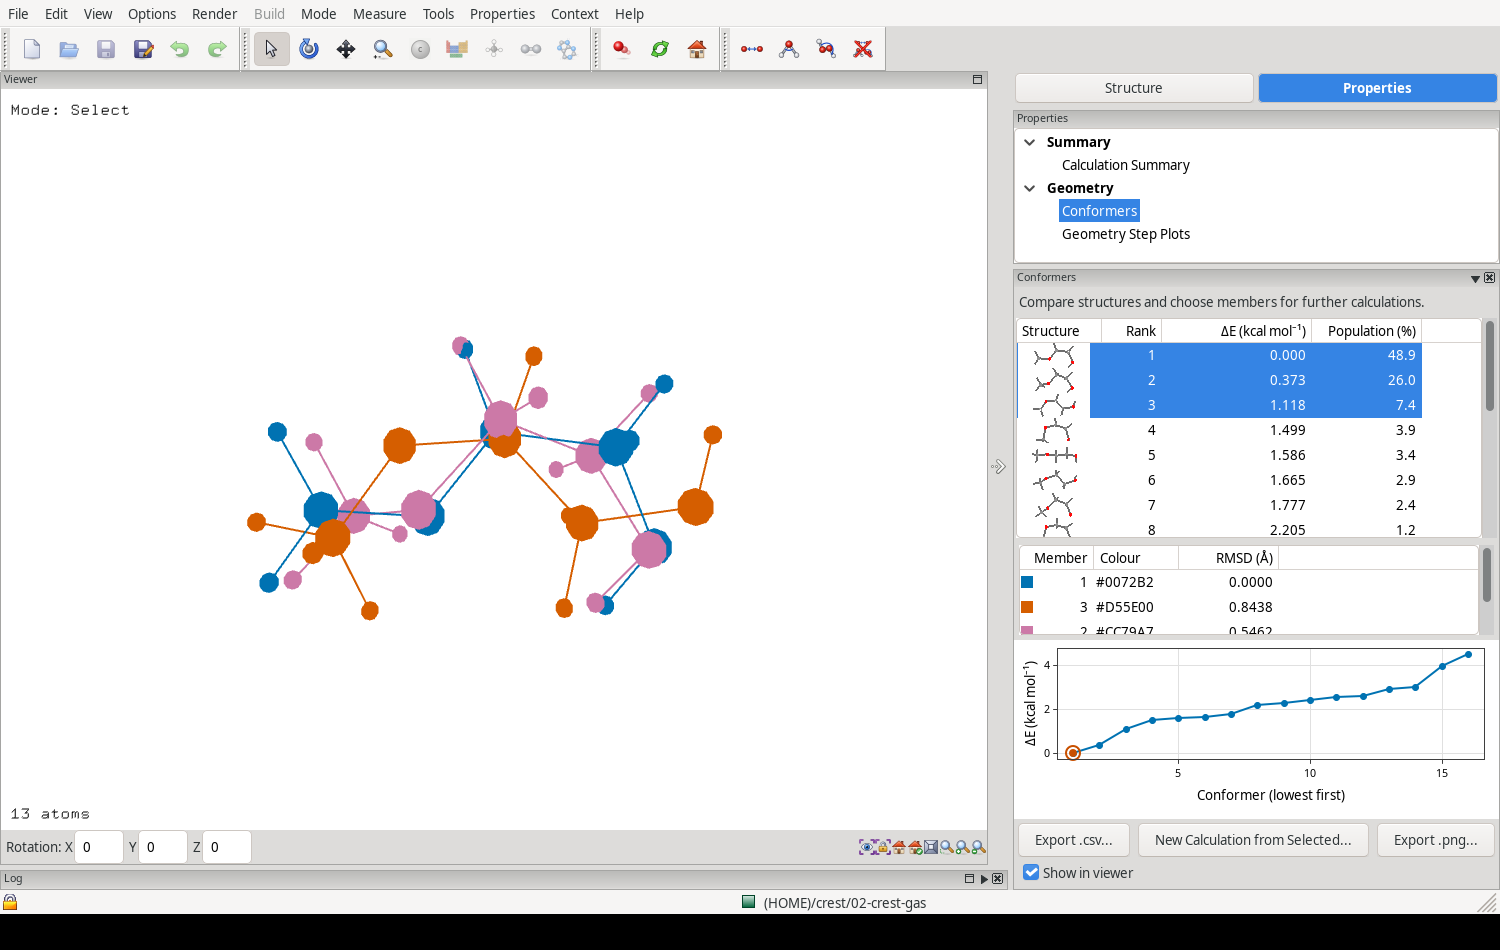
\includegraphics[width=\linewidth]{crest/conformers-overlay.ecce-9.5.3-dev.png}
	\caption{Ranks 1, 2 and 3 of the gas-phase search, fitted onto rank 1 (blue). The key under the table gives the heavy-atom RMSD of each member to the reference.}
	\label{fig:crest-overlay}
\end{figure}

\subsection{The same search with implicit water}
The second search, with ALPB water, took 201~s and also kept 16 conformers. Its lowest structure is again a \emph{gauche} conformer with the hydrogen bond (the hydrogen to oxygen distance is \SI{2.53}{\angstrom}), but the weight of the conformers with a hydrogen to oxygen distance below \SI{2.6}{\angstrom} falls from 77 to 50~percent, and that of the \emph{anti} conformers rises from 15 to 29~percent. We read this as a comparison of structures within each search. The energies of the two searches belong to different models and are not subtracted from one another. The implicit solvent also treats water as a continuum, so the shift tells us that a polar medium weakens the preference for the internal bond, and it cannot tell us what the explicit hydrogen bonds to water molecules do. For that the \menu{Solvation Shell} run type of Chapter~\ref{ch:pom-solvation} is the tool.

One sentence is what the example shows chemically: in the gas phase about three quarters of 2-methoxyethanol sits in a hydrogen-bonded ring, and a continuum model of water already moves a good part of that weight to the extended forms.

\subsection{What to take on}
Before going further we have to decide how many conformers justify a better calculation. The ranking of a tight-binding method is not reliable to a few tenths of a kcal/mol, which means that a cut at the lowest conformer would be a gamble. Chapter~\ref{ch:coupling} shows this for ibuprofen, where the conformer that the best method puts first is the fourth of the cheap one, and it recommends passing on every conformer within the uncertainty of the cheap method and a few more besides. Here the weights give a natural choice. The eight conformers of Table~\ref{tab:crest-gas} carry 96~percent of the ensemble, and since several of them differ only by a methyl rotation, \cmd{ecce-ensemble pick} would merge them into the distinct structures before we spend any density functional time. We ran no higher level for this chapter. For the ranking of the structures at that level, Chapter~\ref{ch:coupling} gives the route and the table to compare.
\index{Funnel!choice of the number of structures}\index{Commands!ecce-ensemble}\index{Distinct conformers}

Re-optimising the lowest conformer with GFN2-xTB at the tight level (35~s) left the structure unchanged, which we expected, since CREST uses the same method; an xTB step after a GFN2 search therefore adds nothing, whereas after a GFN-FF search it moves the structures to the minima of the better method.

The calculations are in the repository of this book under \texttt{calculations/crest}.

\section{Coupling with other codes}
\index{Coupling!CREST}

CREST sits at the head of the funnel of Chapter~\ref{ch:coupling}. What feeds it is an optimised structure, and that comes from xTB or from any other code, since a finished calculation hands over its final geometry together with its charge and multiplicity. For a larger molecule the search can start with GFN-FF for a first look, and \menu{GFN2//GFN-FF} does the force-field search and the GFN2-xTB ranking in one calculation at a higher cost.

What the search feeds is the ensemble. \menu{New Calculation from Selected...} starts one calculation per conformer in another code, typically an xTB optimisation and then a density functional calculation in ORCA, and \cmd{ecce-series} does the same for a longer list from a template. We make these hand-offs by hand, since a few conformers do not justify automation. A workflow pays when the chain recurs, as for the protonation sites of an aminopyridine, where CREST, xTB and ORCA run as one unit (Chapter~\ref{ch:workflows}). The structures of the ensemble can also go the other way, towards the solvent: the lowest conformers are the starting points of the solvation shell calculations of Chapter~\ref{ch:pom-solvation}, and \menu{Protonation Sites} and \menu{Tautomers} (Chapter~\ref{ch:protonation}) use the same panel and the same hand-offs for ions and isomers.
\index{New Calculation from Selected}\index{Commands!ecce-series}\index{Workflows}

\chapter{Fast calculations with xTB}
\label{ch:xtb}
\index{xTB}
\index{GFN2-xTB}
\index{GFN-FF}
\index{Semiempirical methods}
\eccexample{Examples > Getting Started}
\helppage{xtb}
\XXX[ chapter to be written]

\section{Background}

\section{What ECCE shows}

\section{Procedure}

\section{Results}

\section{Coupling with other codes}
% What feeds this calculation (a cheaper screen, a structure from another code)
% and what it feeds (refinement, a property from the code best at it); which
% steps a workflow or recipe automates and which are a manual hand-off.


\chapter{Protonation sites and pKa}
\label{ch:protonation}
\index{Protonation}
\index{pKa}
\index{Solvation}
\index{CPCM}
\eccexample{Examples > Workflows > Aminopyridine protonation}

\XXX[ chapter to be written]

\section{Background}

\section{What ECCE shows}

\section{Procedure}

\section{Results}



\part{Inorganic chemistry}
% Part overview, set before the part's first chapter.
\XXX[ part overview to be written: the kinds of calculations and projects
Inorganic chemistry research does (one paragraph each, e.g. what is computed and why),
and for each the ECCE route and the chapter that shows it (chapters \ref{ch:organometallics}, \ref{ch:ligand-field}, \ref{ch:fragment-orbitals}),
including where ECCE couples codes.]


\chapter{Organometallic and coordination compounds}
\label{ch:organometallics}
\index{Organometallics}
\index{Ligand field}
\index{Coordination compounds}
\index{Spin states}
\eccexample{Examples > Inorganic Chemistry}
\helppage{organometallics}
\XXX[ chapter to be written]

\section{Background}

\section{What ECCE shows}

\section{Procedure}

\section{Results}


\chapter{Ligand field splitting from a calculation}
\label{ch:ligand-field}
\index{Ligand field}
\index{Crystal field}
\index{d-orbital splitting}
\index{Octahedral complexes}
\eccexample{Examples > Inorganic Chemistry}

\XXX[ chapter to be written]

\section{Background}

\section{What ECCE shows}

\section{Procedure}

\section{Results}

\section{Coupling with other codes}
% What feeds this calculation (a cheaper screen, a structure from another code)
% and what it feeds (refinement, a property from the code best at it); which
% hand-off is made (usually by hand: a new calculation from this one's
% structure or orbitals in another code); a workflow only where it pays.


\chapter{A polyoxometalate in water: explicit water molecules and counter ions}
\label{ch:pom-solvation}
\index{Polyoxometalates}
\index{Explicit solvation}
\index{Counter ions}
\index{Solvation shell}
\index{CREST!QCG}
\index{Microsolvation}
\eccexample{Examples > Inorganic Chemistry}
\helppage{recipes}
\XXX[ chapter to be written]

\section{Background}

\section{What ECCE shows}

\section{Procedure}

\section{Results}

\section{Coupling with other codes}
% What feeds this calculation (a cheaper screen, a structure from another code)
% and what it feeds (refinement, a property from the code best at it); which
% steps a workflow or recipe automates and which are a manual hand-off.


\chapter{Fragment orbitals, DOS and OPDOS}
\label{ch:fragment-orbitals}
\index{Fragment orbitals}
\index{Density of states}
\index{OPDOS}
\index{ecce-fragorb}
\index{Interaction diagram}
\eccexample{Examples > Inorganic Chemistry}
\helppage{density-of-states-opdos}
\XXX[ chapter to be written]

\section{Background}

\section{What ECCE shows}

\section{Procedure}

\section{Results}

\section{Coupling with other codes}
% What feeds this calculation (a cheaper screen, a structure from another code)
% and what it feeds (refinement, a property from the code best at it); which
% hand-off is made (usually by hand: a new calculation from this one's
% structure or orbitals in another code); a workflow only where it pays.



\part{Biochemistry}
% Part overview, set before the part's first chapter.
\XXX[ part overview (chapter to be written): the kinds of calculations and projects
Biochemistry research does (one paragraph each, e.g. what is computed and why),
and for each the ECCE route and the chapter that shows it (chapters \ref{ch:docking}, \ref{ch:umbrella} and \ref{ch:protein-md}; fibre patterns of DNA and proteins are in the Teaching part, Chapter~\ref{ch:t-photograph-51}),
including where ECCE couples codes.]


\chapter{Docking a ligand with AutoDock Vina}
\label{ch:docking}
\index{Docking}
\index{AutoDock Vina}
\index{PDBQT}
\index{Docking box}
\index{Poses}
\index{Select Protein}
\index{Select Ligand}
\eccexample{Examples > Biochemistry}
\helppage{vina}
\XXX[ chapter to be written]

\section{Background}

\section{What ECCE shows}

\section{Procedure}

\section{Results}

\section{Coupling with other codes}
% What feeds this calculation (a cheaper screen, a structure from another code)
% and what it feeds (refinement, a property from the code best at it); which
% steps a workflow or recipe automates and which are a manual hand-off.


\chapter{Free energy profiles by umbrella sampling}
\label{ch:umbrella}
\index{Umbrella sampling}
\index{PMF}
\index{WHAM}
\index{Pull force}
\index{ecce-umbrella}
\eccexample{Examples > Biochemistry}
\checkedwith{9.5.3-dev}{4c8b4b851}
\helppage{umbrella-sampling}
\helppage{gromacs-prepare}
\helppage{gromacs-md-settings}

How strongly do two molecules hold on to each other in solution? A single minimisation cannot say, because the answer is a free energy: it includes the water that has to move out of the way, the entropy the two partners lose when they stick, and every arrangement the system can take at room temperature. Umbrella sampling gets it from molecular dynamics. It walks the two partners apart along a distance, holds them at a series of separations long enough to sample each, and combines the results into the free energy as a function of the distance, the \emph{potential of mean force} (PMF). The depth of its minimum below the plateau at large distance is the binding free energy. This chapter does it twice, first for a sodium and a chloride ion in water, which takes minutes and has a well-known answer, and then for one chain of an amyloid fibril pulled off the end of the fibril, the case a protein lab usually asks for.

\section*{This requires}
\index{Requirements!GROMACS}
GROMACS (on Debian, \texttt{sudo apt install gromacs}), registered on the machine that runs the jobs. The ion pair runs on a desktop computer; the fibril is best run on a cluster (Chapter~\ref{ch:hpc}).

\section{Background}
\index{Potential of mean force}\index{WHAM}
If we simply ran a simulation of the ion pair and counted how often each distance occurs, the free energy would follow from the populations, $G(r) = -RT\ln P(r)$, but the system would spend nearly all its time in the deepest minimum and almost never visit the barrier, so the profile would be unknown exactly where it is most interesting. Umbrella sampling fixes this by adding a harmonic spring, the ``umbrella'', that holds the distance near a chosen value in each of a series of \emph{windows}. Each window then samples a narrow range well, including ranges the free system would avoid, and the weighted histogram analysis method (WHAM) removes the known effect of the springs and joins the windows into one profile. This only works if neighbouring windows overlap, so that the histograms can be matched where they share distances, and the spacing of the windows and the stiffness of the springs are chosen with that in mind.

In ECCE the procedure has three steps, all in one GROMACS study. A \emph{pull run} drags one group away from the other at a slow, steady rate, and its trajectory passes through every distance we want. \emph{Windows} are cut from the pull trajectory at a chosen spacing, and each is equilibrated and run with its spring centred on its own distance. \emph{WHAM} then combines the windows' histograms into the PMF.

\section{Sodium chloride in water}
\index{Ion pair}\index{NaCl in water}
Our first system is one \chem{Na+} and one \chem{Cl-} in a 3.2~nm box of TIP3P water, which is small enough to run on a laptop. In water the ions do not simply attract each other as in the gas phase: they meet either in contact, or with one layer of water between them, and these two arrangements are separated by a barrier where the water has to leave.
\begin{enumerate}
	\item Make a GROMACS MD study with a Prepare, an Optimize, an Equilibrate and a Dynamics task, as in Chapter~\ref{ch:liquids}. In the Prepare, place the two ions in contact in the water box, with the AMBER99SB-ILDN force field and TIP3P water.
	\item Run the minimisation, then a constant-pressure (NPT) equilibration in which the two ions are held at contact.
	\item In the Dynamics task's run settings, define the two ions as groups and tick \menu{Pull group 2 away from group 1}, with the coordinate \menu{distance}, a rate of 0.01~nm/ps and a force constant of 1000~kJ/mol/nm$^2$; tick \menu{Write trajectory (.xtc)} with a frequent enough interval to have a frame every few hundredths of a nanometre. Run it until the ions are 1.3~nm apart.
	\item Open the pull run's \menu{Pull Force} panel in its Properties and check that the distance grows steadily with time. On its \menu{Umbrella sampling} page, set \menu{Spacing} to 0.04~nm (an ion pair needs closer windows than a protein), choose \menu{Find windows}, set the equilibration and production steps (5~ps and 100~ps per window here), and choose \menu{Create window calculations}.
	\item Select the window tasks in the Organizer and choose \menu{Run Mgmt > Launch Selected}. The windows are independent of each other and can run side by side.
	\item When they are complete, choose \menu{Run WHAM} on the same page, and tick \menu{Remove the 2RT ln r volume term} (below).
\end{enumerate}
\XXX[run: confirm the Prepare steps for two ions in a water box (Prepare source and placement) and the spring constant actually used; figures: Pull Force, histograms, PMF]

ECCE's own test of this procedure, with 24 windows from 0.24 to 1.2~nm and a spring of 6000~kJ/mol/nm$^2$, gives the profile we expect: the contact ion pair at 0.27~nm, about $-7$~kJ/mol below the separated ions, a barrier at 0.37~nm, about $+8$~kJ/mol, and the solvent-separated pair at 0.52~nm, close to zero. Windows of 100~ps leave about 1~kJ/mol of noise on the curve, which is why ECCE lists only the minima and maxima that differ from their neighbours by more than $RT$.

Note the volume term. Along a distance between two centres, a shell of radius $r$ has an area proportional to $r^2$, so there is simply more room at larger distances, and \texttt{gmx wham} leaves this entropy in its profile. Ticking \menu{Remove the 2RT ln r volume term} removes it and gives the PMF of the pair itself, which is the curve usually published for an ion pair and is flat at large distance. Note also the histograms under the PMF: neighbouring windows must overlap, and ECCE warns, naming the distance, where two of them share less than 5\,\% of their distances. The remedy is a window at that distance, made by running \menu{Find windows} again with a smaller spacing over that range.

\section{One chain off an amyloid fibril}
\index{Amyloid}\index{2BEG}
The second system is the fibril of five A$\beta$(17--42) chains in the PDB entry 2BEG, a widely used test case for umbrella sampling of proteins. We pull chain~A off the end of the fibril while chain~B, its neighbour, is restrained, and ask how much free energy holds the end chain to the fibril.
\begin{enumerate}
	\item In a new GROMACS MD study, set the \menu{Prepare} to \menu{Source: Protein} with the first model of 2BEG, the force field \texttt{gromos53a6}, water \texttt{spc}, \menu{Ignore hydrogens} ticked and \menu{Merge chains into one molecule} unticked, so that each chain keeps its own restraints. Give the box a \menu{Box size (x y z)} of \texttt{6.560 4.362 12} and a \menu{Solute centre (x y z)} of \texttt{3.280 2.181 2.4775}: the fibril sits near one end of a box that is long along $z$, the direction of the pull. Tick \menu{Neutralise} and add 0.1~mol/L NaCl. Launch.
	\item Minimise with steepest descent (at most 50\,000 steps, with \texttt{emtol = 1000} under the extra lines), then equilibrate at constant pressure and 310~K with every chain restrained (\menu{Restrain chain A} to \menu{E}); 100~ps is enough for the box to settle.
	\item In the Dynamics task, restrain chain~B only, define the groups \texttt{Chain\_A = mol:Protein\_chain\_A} and \texttt{Chain\_B = mol:Protein\_chain\_B}, and pull group~2, \texttt{Chain\_A}, away from group~1, \texttt{Chain\_B}, along \menu{distance} at 0.01~nm/ps with $k = 1000$~kJ/mol/nm$^2$. Add the extra lines \texttt{pull-coord1-dim = N N Y}, to pull along $z$ only, and \texttt{nstxout-compressed = 2500}, a frame every 5~ps. 400~ps take chain~A from 0.45~nm to about 5~nm.
	\item In the pull run's \menu{Pull Force} panel, check the force and distance plots, and use \menu{RMSD...} and \menu{Radius of gyration...} to see whether the chain stayed folded while it was pulled. Then cut windows every 0.1~nm, create the window calculations, launch them, and run WHAM as before.
\end{enumerate}
\XXX[run on Kebnekaise: wall time of the pull and of the windows; PMF with its plateau; binding free energy; figures]

The binding free energy is read as the depth of the deepest minimum below the plateau at large distance, and only if the PMF has levelled off there. If it is still rising where the sampling stops, the chain has not yet been pulled far enough, and the pull has to be repeated in a longer box. Note that the shortest distance GROMACS measures is through the periodic box, so a pull cannot go beyond half the box length, which is why the box is long in the direction of the pull and the fibril sits near one end.

\section{Coupling with other codes}
The free energy from umbrella sampling is what docking (Chapter~\ref{ch:docking}) can only estimate, and the two are often used together: docking proposes a pose, and umbrella sampling measures how strongly it binds. The windows are independent jobs, so they are the natural part of the workflow to send to a cluster, while the preparation and the analysis stay on the desktop.

\chapter{Analysing a protein simulation}
\label{ch:protein-md}
\index{MD Analysis}
\index{RDF}
\index{RMSD}
\index{Radius of gyration}
\index{Hydrogen bonds}
\index{ecce-gmxanalysis}
\eccexample{Examples > Computational > GROMACS}
\helppage{md-analysis}
\XXX[ chapter to be written]

\section{Background}

\section{What ECCE shows}

\section{Procedure}

\section{Results}

\section{Coupling with other codes}
% What feeds this calculation (a cheaper screen, a structure from another code)
% and what it feeds (refinement, a property from the code best at it); which
% steps a workflow or recipe automates and which are a manual hand-off.



\part{Materials chemistry}
% Part overview, set before the part's first chapter.
\checkedwith{9.5.3-dev}{a9b2d49c8}

Materials chemistry works with periodic structures, crystals, surfaces and layered solids, and with liquids and other disordered systems, so that the unit of calculation is a cell rather than a molecule. The questions are about structure, stability and transport: whether a structure is stable and what its lattice parameters are, how it responds to strain, what its diffraction pattern looks like, how atoms and ions move through it, and how it interacts with water or with other species between its layers.

The starting point is a structure, and Chapter~\ref{ch:crystals} shows how one is built from scratch or imported from a CIF file, how a supercell is made, and what ECCE shows of the cell. Periodic electronic structure is done with plane waves in Quantum ESPRESSO or with Gaussian basis sets in CP2K. The settings of a plane-wave calculation (the cutoff, the $k$-points and the pseudopotentials) are unfamiliar to anyone used to molecular codes, and Chapter~\ref{ch:qe-settings} says how to choose them, while Chapter~\ref{ch:cp2k} covers periodic structures in CP2K. When the cell itself should relax, the stress tensor tells us in which direction, and Chapter~\ref{ch:stress} shows how it is read and used.

Periodic DFT is expensive, and the screening pattern of the organic chapters applies here too. Machine-learned potentials such as MACE give energies, forces and stresses for a cell in seconds, so that many candidate structures, sites or substitutions can be ranked before the few that matter are refined with Quantum ESPRESSO or CP2K (Chapter~\ref{ch:mlp}). As elsewhere, only the ranking is carried over, not the energies.

Diffraction connects a model with measurements. From any structure in the Builder, ECCE calculates powder patterns, single-crystal reciprocal-lattice sections and detector frames, fibre patterns, and Debye scattering for molecules and clusters, so that a model can be checked against an X-ray measurement without leaving ECCE (Chapter~\ref{ch:diffraction}).

Liquids and interfaces need molecular dynamics. Chapter~\ref{ch:liquids} runs liquids in GROMACS and analyses their density, structure and diffusion, and Chapter~\ref{ch:clays} builds a layered mineral with the Layer Builder, adds interlayer cations and water, types it with the MINFF force field and runs it in GROMACS, which is also an example of a structure built in one place and simulated in another.

\chapter{Crystal structures: building, CIF import and periodic models}
\chaptermark{Crystal structures}
\label{ch:crystals}
\index{Crystal structures}
\index{CIF}
\index{Unit cell}
\index{Supercell}
\index{Periodic models}
\eccexample{Examples > General Chemistry > Packing in solids}
\checkedwith{9.5.3-dev}{4c8b4b851}
\helppage{qe-first-calculation}
\helppage{importing-a-structure}
\helppage{layer-builder}

Every periodic calculation starts from a cell and the atoms in it, and getting these right is half the work: a wrong space group, a missing hydrogen or a partly occupied site taken literally gives a model that no amount of computing will repair. There are three ways to a crystal structure in ECCE. A simple crystal can be built from its space group and the few atoms of its asymmetric unit, a known structure is imported from a CIF file, and a larger model, a supercell, a slab or a stack of layers, is made from a unit cell. This chapter goes through all three, using the solids that ship with ECCE, and ends with the step back from a periodic model to a molecule, a cluster cut out of the crystal.

\section*{This requires}
\index{Requirements!nothing beyond ECCE}
Nothing beyond ECCE for building and inspecting. A CIF file of the crystal you want, for example from the Crystallography Open Database (\url{https://www.crystallography.net}), which is free; ECCE cannot yet search databases itself.

\section{Looking at packed solids}
\index{Packing in solids}\index{Close packing}
In the Organizer, choose \menu{File > Open Example Calculations...}, tick \menu{General Chemistry} and open the topic \menu{Packing in solids}. It holds five metals, each stored as its conventional cell: simple cubic polonium, body-centred cubic sodium, face-centred cubic aluminium and copper, and hexagonal close-packed magnesium. Open one in the Builder and choose \menu{Render > CPK}, which draws the atoms as touching spheres. The Builder draws the atoms on the corners, edges and faces of the cell again at every equivalent position, for display only, so that the packing can be seen as a textbook shows it; each example's note gives the number of atoms in the cell, the nearest neighbours and the fraction of space filled, 52, 68 and 74\,\% for the simple, body-centred and close-packed arrangements. The topic \menu{Molecular and covalent solids} adds crystals held together by hydrogen bonds (ice, urea, sucrose), by dispersion (dry ice, benzene), by a covalent network (diamond) and by covalent layers held together by dispersion (graphite).

\section{Building from a space group}
\index{Periodic Builder}\index{Space group}\index{Asymmetric unit}
A crystal with few atoms in its asymmetric unit is quickest to build directly. Chapter~\ref{ch:qe-settings} builds silicon this way: one silicon atom placed in the Builder, \menu{Tools > Periodic Builder}, \menu{Create Lattice}, the cell lengths and angles typed in \emph{before} any atoms are generated, then the space group typed next to \menu{Sym. Group} and \menu{Generate}, which makes all eight atoms of the cubic cell from the one. Two things decide whether this works. The cell has to be set first, since the atom positions are fractions of it, and the atoms placed have to be exactly the symmetry-distinct ones, since \menu{Generate} adds every image the space group produces and an atom placed twice ends up doubled.

\section{Importing a CIF}
\index{CIF import}
\begin{enumerate}
	\item Download the CIF of the crystal, for example $\alpha$-quartz from the Crystallography Open Database.
	\item Make a calculation for the code you intend to use (Quantum ESPRESSO, CP2K, MACE), open the Builder on it, choose \menu{File > Add Structure from File...}, select \menu{Local Filesystem}, and open the file.
	\item ECCE builds the whole unit cell from the atoms and symmetry operations in the file, or from the space-group name if the file lists no operations, and draws the cell.
	\item Read the Builder's message area. It warns about partly occupied sites (of a site shared by several species, the one with the highest occupancy is kept), about a structure without hydrogen atoms, and about a file with more than one data block, of which only the first is read.
	\item Save.
\end{enumerate}
\XXX[run: quartz from COD as the worked example; atom count and cell after import; figure]

The warnings matter. X-ray structures often lack hydrogens, which then have to be added before any calculation, and a disordered site in the file describes an average over many unit cells that no single periodic model can reproduce, so the highest-occupancy choice is a starting point to be thought about, not a result. \menu{File > Save As...} with the type \emph{CIF, P1} writes the cell and every atom without symmetry, which reads back as the same structure and is the form most other programs accept.

\section{Larger cells}
\index{Supercell}\index{Replicate}\index{Layer Builder}
A defect, a substitution or a dilute dopant needs a cell larger than the unit cell, so that the defect is far enough from its own periodic images. In the Periodic Builder, \menu{Replicate} repeats the cell along $a$, $b$ and $c$ the given number of times, and \menu{Unit Cell} goes back. For layered materials, the Layer Builder (\menu{Tools > Layer Builder}) stacks a layer with chosen spacings and shifts and fills the gaps with ions and water; Chapter~\ref{ch:clays} uses it for a clay. Note that every atom of a supercell is computed, so the cost of a DFT calculation grows quickly with its size, which is one reason to screen large cells with a machine-learned potential first (Chapter~\ref{ch:mlp}).

\section{From a crystal to a cluster}
\index{Cut Cluster}
Some properties are better computed with a molecular code, which needs a finite cluster. \menu{Build > Cut Cluster...} cuts one out of a periodic structure: select the atom or atoms to centre on, enter a radius, and choose whether to cut through bonds, keep whole molecules, or, for an ionic crystal, keep whole formula units so that the cluster stays neutral. \menu{Capping} closes the bonds the cut severed with hydrogen atoms or hydroxyl groups, along the direction of each bond. The result replaces the periodic structure, and \menu{Edit > Undo} brings it back.

\section{Coupling with other codes}
A structure built or imported here is the input for the periodic codes, Quantum ESPRESSO, CP2K and MACE (Chapters~\ref{ch:qe-settings}, \ref{ch:cp2k} and \ref{ch:mlp}), and for its calculated diffraction pattern (Chapter~\ref{ch:diffraction}), which is the quickest check that an imported structure is the one in the paper. A cluster cut from it goes to a molecular code.

\chapter{Liquids by MD: density, diffusion and structure}
\label{ch:liquids}
\index{GROMACS}
\index{Liquids}
\index{Diffusion coefficient}
\index{RDF}
\index{Density}
\eccexample{Examples > General Chemistry > Gases, liquids and solids}
\helppage{gromacs-first-calculation}
\helppage{md-speeds-and-diffusion}
\XXX[ chapter to be written]

\section{Background}

\section{What ECCE shows}

\section{Procedure}

\section{Results}


\chapter{Powder, single-crystal and fibre diffraction from a model}
\label{ch:diffraction}
\index{Powder pattern}
\index{Single crystal}
\index{Precession photograph}
\index{Detector frame}
\index{Fibre diffraction}
\index{Debye scattering}
\eccexample{Examples > General Chemistry > Diffraction}
\helppage{fibre-diffraction}
\XXX[ chapter to be written]

\section{Background}

\section{What ECCE shows}

\section{Procedure}

\section{Results}


\chapter{Periodic DFT with Quantum ESPRESSO}
\label{ch:qe-settings}
\index{Quantum ESPRESSO}
\index{k-points}
\index{Cutoff}
\index{Pseudopotentials}
\index{vc-relax}
\eccexample{Examples > General Chemistry > Packing in solids}
\helppage{qe-choosing-settings}
\XXX[ chapter to be written]

\section{Background}

\section{What ECCE shows}

\section{Procedure}

\section{Results}


\chapter{Periodic structures in CP2K}
\label{ch:cp2k}
\index{CP2K}
\index{GTH pseudopotentials}
\index{SCF convergence}
\eccexample{Examples > Getting Started}
\helppage{cp2k-scf}
\helppage{cp2k-basis-potential}
\XXX[ chapter to be written]

\section{Background}

\section{What ECCE shows}

\section{Procedure}

\section{Results}

\section{Coupling with other codes}
% What feeds this calculation (a cheaper screen, a structure from another code)
% and what it feeds (refinement, a property from the code best at it); which
% steps a workflow or recipe automates and which are a manual hand-off.


\chapter{Machine-learned potentials (MACE)}
\label{ch:mlp}
\index{MACE}
\index{Machine-learned potentials}
\index{ML potential}
\index{Site screening}
\eccexample{Examples > Materials Chemistry}
\helppage{mlp}
\XXX[ chapter to be written]

\section{Background}

\section{What ECCE shows}

\section{Procedure}

\section{Results}

\section{Coupling with other codes}
% What feeds this calculation (a cheaper screen, a structure from another code)
% and what it feeds (refinement, a property from the code best at it); which
% steps a workflow or recipe automates and which are a manual hand-off.


\chapter{Clay minerals: layers, interlayer water and MINFF}
\label{ch:clays}
\index{Layer builder}
\index{Clay minerals}
\index{MINFF}
\index{atomipy}
\index{Interlayer}
\index{Basal spacing}
\index{Isomorphic substitution}
\index{Montmorillonite}
\eccexample{Examples > Materials Chemistry > Clays}
\helppage{layer-builder}
\helppage{gromacs-prepare}
\XXX[ chapter to be written]

\section{Background}

\section{What ECCE shows}

\section{Procedure}

\section{Results}


\chapter{Stress and cell relaxation}
\label{ch:stress}
\index{Stress tensor}
\index{Pressure}
\index{Cell relaxation}
\eccexample{Examples > Materials Chemistry}

\XXX[ chapter to be written]

\section{Background}

\section{What ECCE shows}

\section{Procedure}

\section{Results}



\part{Teaching}
\chapter{Teaching with ECCE}
\label{ch:teaching}
\index{Teaching}
\index{Example sets}
\index{Central server}
\eccexample{Examples > General Chemistry}
\helppage{molecules-for-teaching}
\XXX[ chapter to be written: for teachers. The example sets by topic, the
teaching MO diagram, ECCE-QM in class, a central server for a class. The chapters
after this one are worked class demonstrations.]

\section{Atomic orbitals: radial distributions and slices}
\label{sec:atomic-orbitals}
\index{Atomic orbitals}
\index{Orbitals!atomic|see{Atomic orbitals}}
\index{Argon}
\checkedwith{9.5.3-dev}{9aa88a4ce}
\eccexample{Examples > General Chemistry > Atoms}
\helppage{density-profile}

\helppage{density-map}

The orbitals of an atom are usually drawn as boundary surfaces, a sphere for s and two lobes for p, and such a drawing hides most of what the principal quantum number does. This chapter looks at the occupied orbitals of argon in two other ways, as a curve of probability against the distance from the nucleus and as a contour map on a flat slice through the nucleus. Both views come from the same stored calculation and show the nodes, the inner maxima of 2s, 3s and 3p, and the three shells of argon.
\index{Shells}\index{Nodes}\index{Inner maxima}

\subsection{Background}
\index{Radial distribution}
\index{Radial distribution function|see{Radial distribution}}
\index{Orbitals!radial distribution|see{Radial distribution}}
\index{Probability of finding an electron|see{Radial distribution}}
An orbital $\psi(r,\theta,\phi)$ of an atom gives, through $|\psi|^2$, the probability per unit volume of finding the electron at a point. The question asked of an atom is more often how far from the nucleus the electron is, in any direction, and the answer is the radial distribution function
\begin{equation}
	P(r) = r^2 \oint |\psi(r,\theta,\phi)|^2 \, d\Omega ,
	\label{eq:rdf}
\end{equation}
the probability per unit distance of finding the electron in a thin spherical shell of radius $r$. For a normalised orbital $\int_0^\infty P(r)\,dr = 1$. For a hydrogen-like atom the orbital separates into a radial part $R_{nl}(r)$ and a spherical harmonic, and Eq.~\eqref{eq:rdf} reduces to $P(r) = r^2 R_{nl}^2(r)$. The factor $r^2$, which is the area of the sphere apart from $4\pi$, makes $P(r)$ zero at the nucleus even for an s orbital, whose density $|\psi|^2$ is largest there.

The radial part has $n-l-1$ nodes, spheres on which $\psi$ is zero and changes sign, and the orbital has $l$ angular nodes besides, planes or cones through the nucleus, so $n-1$ nodes in all.
\index{Nodes!radial}\index{Nodes!angular}\index{Nodal plane}
Between consecutive radial nodes $P(r)$ has a maximum, which gives $n-l$ maxima: one for 1s, 2p and 3d, two for 2s and 3p, three for 3s. The outermost maximum is the largest and sets the size of the orbital; the others are the inner maxima. The position of the largest maximum is the most probable radius,
\index{Most probable radius}\index{Inner maxima}
which for a hydrogen-like orbital with $l = n-1$, one without a radial node, is
\begin{equation}
	r_\mathrm{mp} = \frac{n^2 a_0}{Z},
	\label{eq:rmp}
\end{equation}
with $a_0 = \SI{0.529}{\angstrom}$ the Bohr radius and $Z$ the nuclear charge; for 1s it is $a_0/Z$.

The inner maxima are the origin of penetration.
\index{Penetration}\index{Shielding}
A 2s electron has a small maximum inside the 1s shell, close to the nucleus, where the two 1s electrons screen little of the nuclear charge, and a 2p electron has no such maximum. The 2s electron therefore feels a larger effective nuclear charge on average and lies lower in energy, which is why 2s fills before 2p and, in the next period, 3s before 3p (Section~\ref{sec:periodic-trends}). Slater's screening rules put these trends into numbers \cite{slater1930}.
\index{Effective nuclear charge}

In a many-electron atom the orbitals are no longer hydrogen-like, but the counting of nodes and maxima survives. The total electron density of argon, summed over the occupied orbitals and weighted by $r^2$, has one hump for each filled shell: 1s close to the nucleus, then 2s and 2p together, then 3s and 3p.

\subsection{What ECCE shows}
\index{Density Profile}\index{Density Map}
\index{Properties list!Density Profile}\index{Properties list!Density Map}
The Atoms topic of the General Chemistry example set holds ECCE-QM calculations of 21 atoms, H to Ar, Ca, Cr and Cu.
\index{ECCE-QM}\index{Codes!ECCE-QM}\index{Example calculations!General Chemistry}
The argon calculation uses B3LYP \cite{becke1993} with the aug-cc-pVTZ basis set \cite{woon1993}, is closed shell, and gives a total energy of $-527.490442$~hartree. Its nine occupied orbitals are 1s ($-115.118$~hartree), 2s ($-11.142$), three 2p ($-8.693$), 3s ($-0.968$) and three 3p ($-0.426$).
\index{B3LYP}\index{Basis sets!aug-cc-pVTZ}\index{Orbital energies!argon}

Two panels in the Orbitals group of the \menu{Properties} list work from the orbital coefficients and the basis set stored with the calculation. The \menu{Density Profile} plots a quantity against one length; for a single atom it opens on \menu{Around an atom}, where \menu{Radial distribution} is Eq.~\eqref{eq:rdf} evaluated for each chosen orbital and \menu{Spherical average of $\psi^2$} is the same average without the $r^2$.
\index{Density Profile!Around an atom}\index{Density Profile!Radial distribution}\index{Density Profile!Spherical average of psi2@Spherical average of $\psi^2$}
The \menu{r axis} can be \menu{Linear}, \menu{$\sqrt{r}$} or \menu{log r}; the square root spreads out the region near the nucleus, where the inner shells are, while the tick marks stay in $r$ itself.
\index{Density Profile!r axis}\index{Square-root axis}
On a $\sqrt{r}$ axis the area under a curve is no longer the number of electrons, and the panel says so beneath the plot, where the note also gives the most probable distance of each curve.
\index{Most probable radius!in the Density Profile}

The \menu{Density Map} draws one orbital, or the density, as contour lines on a flat slice. A single atom opens on \menu{This view (parallel to the screen)}, a plane through the nucleus. With \menu{Show: One orbital} the positive values are drawn as solid blue lines and the negative values as dashed vermilion lines, so that a node lies where the two colours meet; the levels start at $\pm 0.02$ and double.
\index{Density Map!One orbital}\index{Density Map!This view (parallel to the screen)}\index{Contour map}\index{Orbitals!sign|see{Phase}}\index{Phase}
The \menu{MO} box chooses the orbital, and the mouse wheel zooms the map about the pointer.

\subsection{Procedure}
\index{Opening example calculations}
\index{File menu!Open Example Calculations}
\index{Organizer!Open Example Calculations}
\index{Viewer}
\begin{enumerate}
	\item In the Organizer, choose \menu{File > Open Example Calculations}, pick \menu{General Chemistry} and click \menu{OK}. The calculations go into the project \menu{Examples}, sorted into topics.
	\item In the topic \menu{Atoms}, select the calculation \menu{Ar} and click \menu{Viewer}.
	\item In the \menu{Properties} list, click \menu{Density Profile}. The panel opens on \menu{Around an atom} with \menu{Centre} \menu{Ar1}.
	\index{Density Profile!Centre}
	\item Choose \menu{Radial distribution} and \menu{Selected orbitals}, and in the list of orbitals tick 1s, 2s and 3s and untick the others.
	\index{Density Profile!Selected orbitals}
	\item Set \menu{r axis} to \menu{$\sqrt{r}$}.
	\item To zoom, turn the mouse wheel over the plot or drag a rectangle; double-click to return to the whole plot, or click \ctrl{Show all}.
	\index{Density Profile!Show all}\index{Zooming a plot}
	\item Tick 2p, 3s and 3p instead.
	\item In the \menu{Properties} list, click \menu{Density Map} and choose \menu{Show: One orbital}.
	\item Step through the occupied orbitals 1 to 9 with the arrows of the \menu{MO} box, drawn as \ctrl{$-$} and \ctrl{+} buttons. The caption above the map names the orbital, its energy and its occupation.
	\index{Density Map!MO box}\index{Stepping through orbitals}
	\item Turn the mouse wheel over the nucleus to zoom in; double-click the map, or click \ctrl{Whole plane}, to see all of it again.
	\index{Density Map!Whole plane}\index{Zooming a map}
\end{enumerate}

\subsection{Results}
\index{Shells!of argon}
Figure~\ref{fig:ao-rdf1} shows the radial distributions of 1s, 2s and 3s on the $\sqrt{r}$ axis. 1s has a single maximum, at a most probable distance of \SI{0.0299}{\angstrom} according to the note under the plot. Equation~\eqref{eq:rmp} with $Z = 18$ gives $a_0/18 = \SI{0.0294}{\angstrom}$, and the slightly larger value is the screening of one 1s electron by the other, corresponding to an effective nuclear charge of about 17.7. 2s has one node and two maxima, the smaller at about the distance of the 1s maximum, and 3s has two nodes and three maxima, the inner two at about the distances of the 1s and 2s maxima. The number of nodes rises by one with each step in $n$. The most probable distances of 2s and 3s are \XXX[ read from the note under the plot].
\index{Effective nuclear charge}

\begin{figure}[htb]
	\centering
	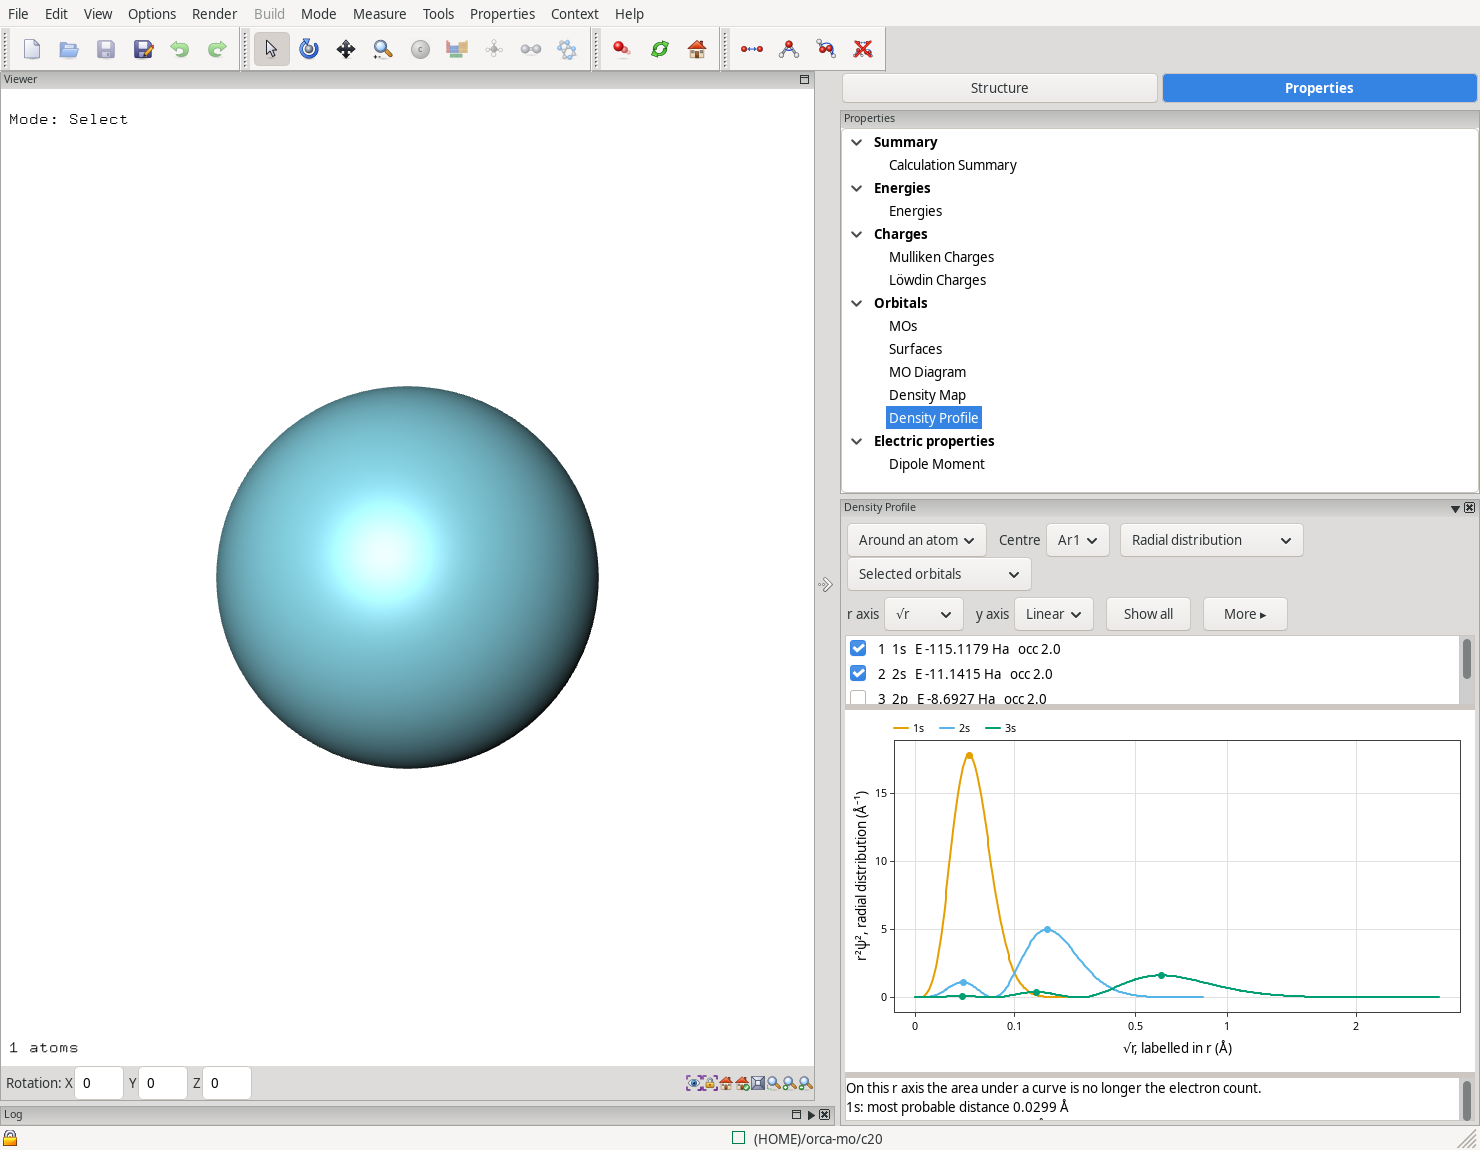
\includegraphics[width=\linewidth]{atomic-orbitals/rdf1.ecce-unknown.png}
	\caption{Argon in the Viewer, with the \menu{Density Profile} on \menu{Around an atom}, \menu{Radial distribution}, \menu{Selected orbitals} 1s, 2s and 3s and a $\sqrt{r}$ axis. \XXX[ screenshot shows a \menu{More} button where the help names \menu{Options}; regenerate from the Atoms example.]}
	\label{fig:ao-rdf1}
\end{figure}

With 2p, 3s and 3p ticked (Fig.~\ref{fig:ao-rdf2}), 2p has a single maximum and no node, and 3p has one node and two maxima. The main maxima of 3s and 3p lie at about the same distance, that of 3p slightly further out, which is what makes them one shell. Their inner maxima differ, since 3p has one, near the 2p maximum, while 3s has a second one closer still to the nucleus, at about the 1s maximum. A 3s electron therefore penetrates further than a 3p electron, and the orbital energies follow, $-0.968$~hartree for 3s against $-0.426$~hartree for 3p.
\index{Penetration!3s and 3p}

\begin{figure}[htb]
	\centering
	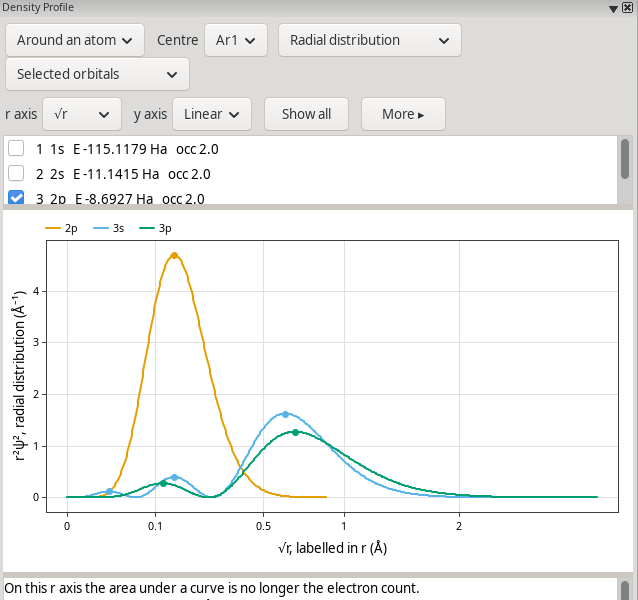
\includegraphics[width=0.75\linewidth]{atomic-orbitals/rdf2.ecce-unknown.png}
	\caption{The \menu{Density Profile} of argon with 2p, 3s and 3p ticked.}
	\label{fig:ao-rdf2}
\end{figure}

The total density of argon, with its three shells, is not among the figures yet. \XXX[ screenshot: Ar, \menu{Density Profile}, \menu{Around an atom}, \menu{Radial distribution}, \menu{Total only}, \menu{r axis} $\sqrt{r}$, showing the three humps of the total for 1s, 2s+2p and 3s+3p.]

In the \menu{Density Map} (Fig.~\ref{fig:ao-map}) orbital 6 is 3s. The circles of the contour map are the spherical nodes of the radial distribution seen edge-on. Going out from the nucleus the sign changes twice, which gives a small disc about the nucleus, a ring of opposite sign around it and the large outer part, with the sign of the disc. The disc and the ring are the two inner maxima of Fig.~\ref{fig:ao-rdf1}, and the zoomed map (Fig.~\ref{fig:ao-mapzoom}) shows how close to the nucleus they lie. The sign of 1s does not change at all, and that of 2s changes once.

\begin{figure}[htb]
	\centering
	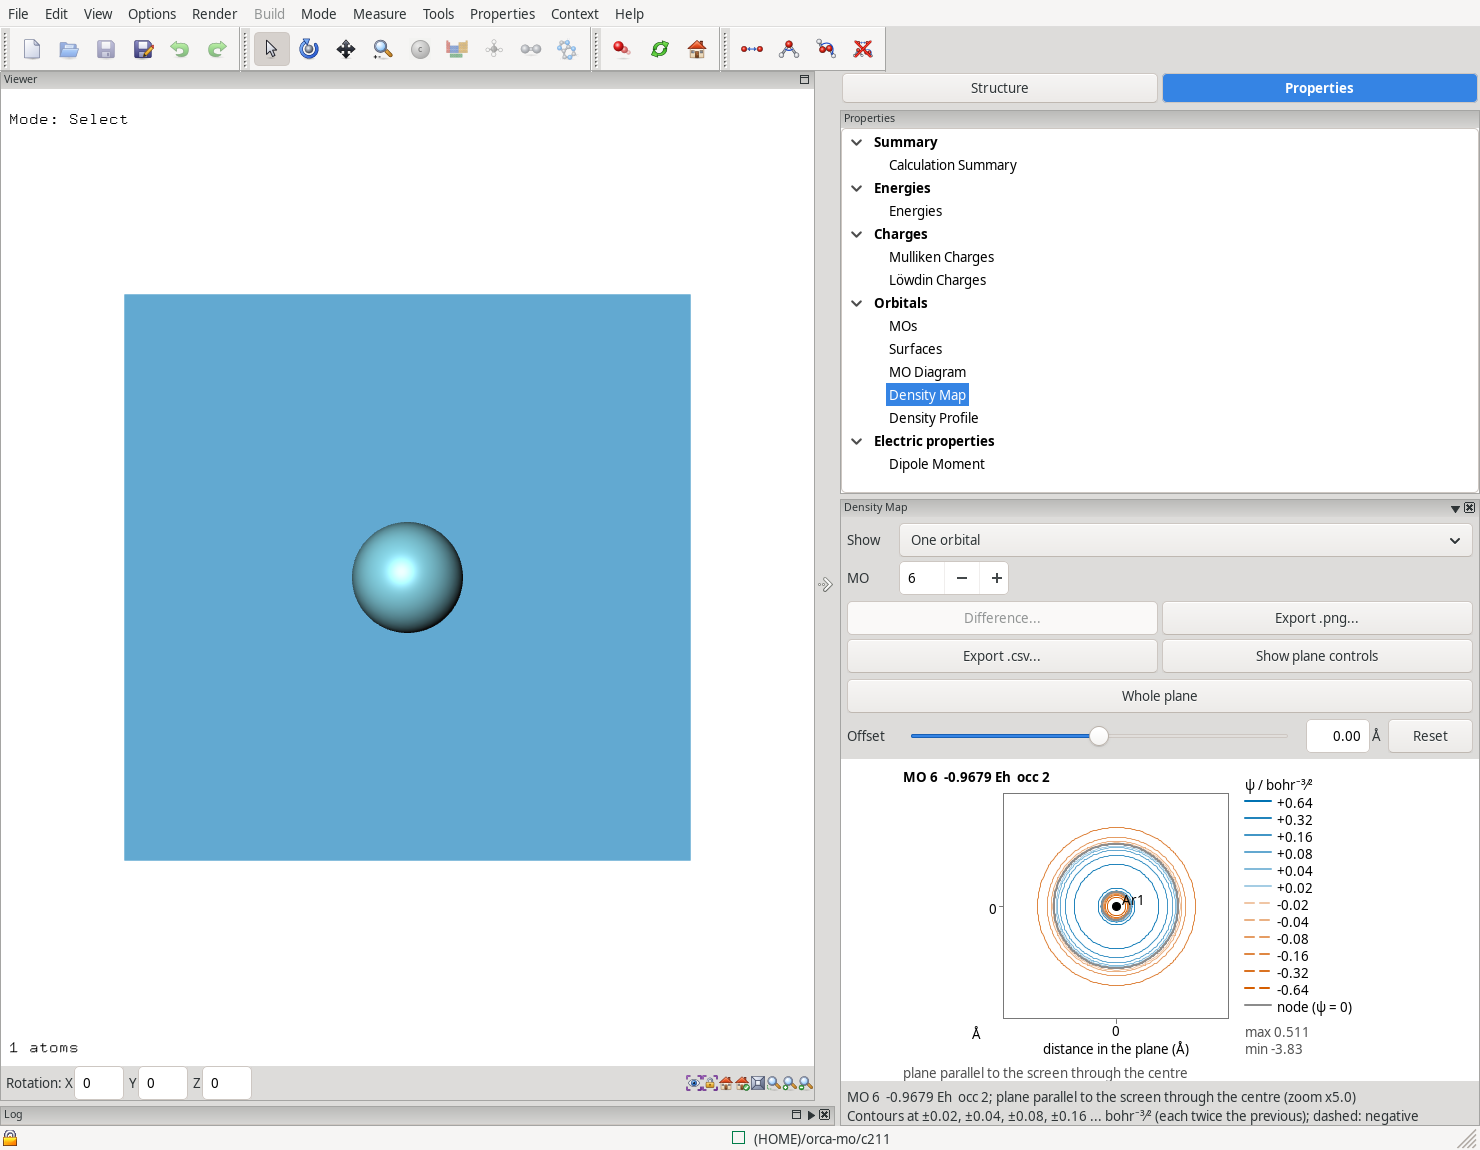
\includegraphics[width=\linewidth]{atomic-orbitals/map1.ecce-unknown.png}
	\caption{Argon with the \menu{Density Map} on \menu{One orbital}, MO 6 (3s, $-0.9679$~hartree), on the plane parallel to the screen through the nucleus; the slice is drawn in the 3-D view as a translucent square. \XXX[ screenshot shows a \menu{Show plane controls} button where the help names \menu{Options}; regenerate.]}
	\label{fig:ao-map}
\end{figure}

\begin{figure}[htb]
	\centering
	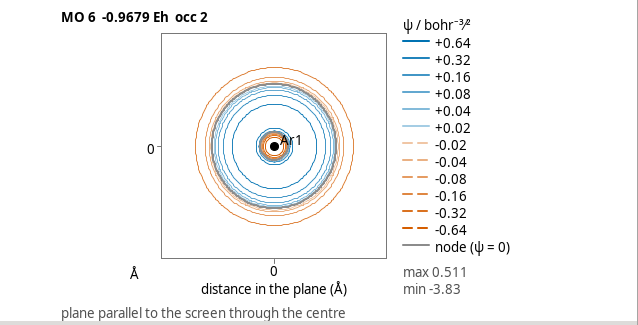
\includegraphics[width=0.75\linewidth]{atomic-orbitals/map1zoom.ecce-unknown.png}
	\caption{The map of Fig.~\ref{fig:ao-map}, zoomed in on the nucleus.}
	\label{fig:ao-mapzoom}
\end{figure}

The 2p and 3p orbitals each have a nodal plane through the nucleus, and the slice cuts the three members of each set differently: a member lying in the slice shows two lobes of opposite sign on either side of the nodal line, while one pointing out of the slice can look almost empty. \XXX[ screenshot: Ar, \menu{Density Map}, \menu{One orbital}, the member of MO 3--5 (2p) that lies in the plane, zoomed in, showing the nodal plane as a line.]
\index{Nodal plane}

\subsection{History}
Schrödinger solved the wave equation of the hydrogen atom in 1926, which gave the radial functions and their nodes \cite{schrodinger1926}, and Slater set out his rules for the screening of the nuclear charge in 1930 \cite{slater1930}.
\index{History!Schrödinger}\index{History!Slater}

\chapter{The periodic table from calculation: configurations, shielding and ionisation}
\sectionmark{The periodic table from calculation}
\label{sec:periodic-trends}
\label{sec:configurations}
\checkedwith{9.5.3-dev}{ce2531fa0}
\index{Periodic trends}
\index{Periodic table|see{Periodic trends}}
\eccexample{Examples > General Chemistry > Atoms}
\helppage{ecce-qm}

The filling order 1s, 2s, 2p, 3s, 3p, 4s, 3d is usually taught as a rule to memorise. Here we read it from calculations instead: the atoms H to Ar, Ca, Cr and Cu, and some of their ions, from the General Chemistry example set. The orbital energies give the configurations and an effective nuclear charge; total energies of atoms and ions give ionisation energies and electron affinities. The rise in ionisation energy across a period, the drop at each alkali metal and the dips at B and O all appear, and so do a few places where the numbers are easy to over-read.
\index{Electron configuration}\index{Configurations|see{Electron configuration}}
\index{Ionisation energy}\index{Ionization energy|see{Ionisation energy}}
\index{Electron affinity}

\section*{This requires}
Nothing beyond ECCE: the calculations are in the General Chemistry example set.

\section{Background}
\index{Aufbau principle}\index{Building-up principle|see{Aufbau principle}}\index{Pauli principle}
\index{Penetration}\index{Shielding}\index{Screening|see{Shielding}}\index{Subshells}
In the orbital picture, the ground state puts the electrons, two per orbital at most, into the orbitals of lowest energy. In hydrogen the energy depends on $n$ alone. In other atoms the electrons screen the nucleus from each other, and an s electron, which penetrates the inner shells, feels more of the nuclear charge than a p electron of the same shell (Chapter~\ref{sec:atomic-orbitals}). The subshells therefore separate, ns below np below nd, and for $n = 3$ and 4 enough that 4s fills before 3d.

\index{Hund's rule}\index{Multiplicity}\index{Spin multiplicity|see{Multiplicity}}
In a partly filled subshell, Hund's first rule puts the electrons in different orbitals with parallel spins. Carbon is then a triplet, nitrogen a quartet, oxygen a triplet again. Note that in a calculation the multiplicity is part of the input: you choose how many electrons are unpaired.

\index{Effective nuclear charge}\index{Zeff@$Z_\mathrm{eff}$|see{Effective nuclear charge}}
The screening can be put into one number, the effective nuclear charge $Z_\mathrm{eff} = Z - S$, where $Z$ is the nuclear charge and $S$ the screening constant. Slater's rules estimate $S$ from the configuration \cite{slater1930}. For an electron in an s or p orbital of shell $n$, every other electron in the same shell contributes 0.35 to $S$ (0.30 within 1s), every electron in shell $n-1$ contributes 0.85, and every electron further in contributes 1.00. For the 2s electron of lithium, $1s^2 2s^1$, the two 1s electrons give $S = 2 \times 0.85 = 1.70$, so that $Z_\mathrm{eff} = 3 - 1.70 = 1.30$. For a 2p electron of neon, $1s^2 2s^2 2p^6$, the seven other $n = 2$ electrons and the two 1s electrons give $S = 7 \times 0.35 + 2 \times 0.85 = 4.15$ and $Z_\mathrm{eff} = 10 - 4.15 = 5.85$.

A second estimate comes from the calculation itself. It treats an orbital of energy $\varepsilon$ as if it were a hydrogen-like orbital of the same $n$, for which $\varepsilon = -Z^2/2n^2$ in hartree, and solves for the charge:
\begin{equation}
	\varepsilon = -\frac{Z_\mathrm{eff}^2}{2n^2}\ \text{hartree}, \qquad
	Z_\mathrm{eff} = n\sqrt{-2\varepsilon/\text{hartree}} .
	\label{eq:zeff}
\end{equation}
The two are not the same thing. An orbital energy contains the repulsion with every other electron, including those of the same shell, and equation~\eqref{eq:zeff} puts all of it into $Z_\mathrm{eff}$.

\index{Koopmans' theorem}\index{Ionisation energy!from orbital energies}\index{Delta SCF@$\Delta$SCF}\index{Relaxation}\index{Electron correlation}\index{HOMO}
The first ionisation energy is $\mathrm{IE} = E(\mathrm{A}^+) - E(\mathrm{A})$, the electron affinity $\mathrm{EA} = E(\mathrm{A}) - E(\mathrm{A}^-)$, positive when the anion is more stable. Both come from two total energies (the $\Delta$SCF route). Koopmans' theorem gives a shortcut for Hartree-Fock: $\mathrm{IE} \approx -\varepsilon_\mathrm{HOMO}$, where HOMO is the highest occupied orbital, if the other orbitals do not change \cite{koopmans1934}. Two errors enter. The remaining electrons relax towards the hole, which makes $-\varepsilon_\mathrm{HOMO}$ too large. Hartree-Fock also leaves out electron correlation, the part of the repulsion between electrons that its average field misses because the electrons in fact avoid each other; the correlation energy is larger in the atom than in the cation and makes the Hartree-Fock IE too small. $\Delta$SCF includes the relaxation but not the correlation. For a density functional such as B3LYP, $-\varepsilon_\mathrm{HOMO}$ is well below the IE.

ECCE gives orbital energies in hartree and the Energy Calculator gives energy differences in kJ/mol, kcal/mol and eV. The conversions used in this chapter are 1~hartree = 27.2114~eV = 2625.50~kJ/mol.

\section{The calculations}
\index{ECCE-QM}\index{Codes!ECCE-QM}\index{Example calculations!General Chemistry}
\index{B3LYP}\index{Basis sets!aug-cc-pVTZ}\index{Basis sets!def2-TZVPD}\index{Basis sets!cc-pVTZ}\index{ROKS}\index{Restricted open shell}
\index{Hartree-Fock}\index{UHF}\index{PBE0}\index{Basis sets!aug-cc-pVDZ}
Three topics of the General Chemistry example set hold the ECCE-QM calculations:
\begin{enumerate}
	\item \menu{Atoms}: the 21 atoms, B3LYP \cite{becke1993}, aug-cc-pVTZ \cite{kendall1992,woon1993} for H to Ar, cc-pVTZ for Ca, def2-TZVPD \cite{rappoport2010} for Cr and Cu. Closed shells are restricted, open shells restricted open-shell (ROKS): the alpha and beta electrons share one set of spatial orbitals. The aug-cc-pVTZ basis is of triple-zeta quality with diffuse functions, which describe the loosely bound outer electrons; cc-pVTZ lacks the diffuse functions, and def2-TZVPD is a triple-zeta basis with diffuse functions from another family.
	\item \menu{Koopmans' theorem}: H to Ar, Hartree-Fock/aug-cc-pVTZ, unrestricted (UHF) for open shells, so that the alpha and beta electrons have orbitals, and orbital energies, of their own.
	\item \menu{Ionisation energies and electron affinities}: Li, Be, C, N, O, F, Ne and their cations (Hartree-Fock/aug-cc-pVTZ); Li, Be, C, N, O, F and their anions (PBE0/aug-cc-pVDZ \cite{adamo1999}).
\end{enumerate}
Each calculation has a note saying what it shows.

\index{MOs panel}\index{Properties list!MOs}\index{MOs panel!Compute}\index{MO Diagram}\index{Properties list!MO Diagram}\index{Orbital energies}
In the Viewer, the \menu{MOs} panel lists the orbitals with their energy and occupation. Select a row and click \ctrl{Compute} to draw the orbital, which tells s from p or d. \menu{Tools > Energy Calculator...} in the Organizer takes two calculations, A then B, and gives \menu{B - A} in kJ/mol, kcal/mol and eV.
\index{Energy Calculator}\index{Tools menu!Energy Calculator...}\index{Energy Calculator!B - A}
\index{Calculating an ionisation energy}\index{Calculating an electron affinity}
\helppage{energy-calculator}

\section{Procedure}
\index{Opening example calculations}\index{File menu!Open Example Calculations}\index{Organizer!Open Example Calculations}\index{Viewer}
\begin{enumerate}
	\item In the Organizer, choose \menu{File > Open Example Calculations}, pick \menu{General Chemistry} and click \menu{OK}.
	\item In \menu{Atoms}, select \menu{Ne}, click \menu{Viewer} and open \menu{MOs}. Read the energies of 1s, 2s and 2p.
	\item Select \menu{Na}, \menu{C}, \menu{N} and \menu{O} in turn. Count the singly occupied orbitals (\menu{Occ \#} 1) and compare with the multiplicity.
	\item Select \menu{Ca}, \menu{Cr} and \menu{Cu}. Find 4s and 3d near the top of the occupied list; \ctrl{Compute} tells which is which.
	\item In \menu{Koopmans' theorem}, open \menu{N\_HF} and \menu{O\_HF} and read the energy of the highest occupied orbital. The \menu{MOs} panel lists the alpha orbitals first and the beta orbitals below them; in an open shell the highest occupied orbital can be a beta one, as in oxygen, so compare the last occupied orbital of each set. Multiply by $-27.2114$ to get the Koopmans IE in eV.
	\index{Koopmans' theorem!in the MOs panel}
	\item In \menu{Koopmans' theorem}, open \menu{Li\_HF}, read \menu{E (Hartree)} of the highest occupied orbital (\menu{Occ \#} 1, the 2s) and calculate $Z_\mathrm{eff} = n\sqrt{-2\varepsilon}$ with $n = 2$ (equation~\eqref{eq:zeff}). Repeat for \menu{Ne\_HF} and \menu{Na\_HF} ($n = 3$), and compare with Slater's rules.
	\index{Effective nuclear charge!calculating}
	\item In \menu{Ionisation energies and electron affinities}, select \menu{N\_HF\_neutral}, Ctrl-click \menu{N\_HF\_cation} and choose \menu{Tools > Energy Calculator...}. \menu{B - A} is the ionisation energy. Repeat for the other pairs.
	\item For an electron affinity, select the anion first (\menu{F\_anion}), then the atom (\menu{F\_PBE0\_neutral}). \menu{B - A} is the electron affinity.
\end{enumerate}

\section{Configurations}
\index{Electron configuration!of the atoms H to Ar}\index{Orbital energies!of the atoms}\index{Penetration!2s and 2p}\index{Neon}\index{Sodium}
Every atom fills its orbitals in the Aufbau order (table~\ref{tab:pt-config}). Neon shows the split of a shell most clearly: 2s at $-1.459$ and 2p at $-0.572$~hartree, 24~eV apart although both have $n = 2$. In sodium the next electron goes into 3s at $-0.125$~hartree, and the 2p has dropped to $-1.156$~hartree, into the core.

\begin{table}[htb]
	\centering\small
	\caption{Atoms H to Ar (B3LYP/aug-cc-pVTZ): multiplicity used, valence configuration and valence orbital energies in hartree. Where singly and doubly occupied p orbitals differ in energy, both are given, singly occupied first.}
	\label{tab:pt-config}
	\begin{tabular}{lcl rr}
		\hline
		Atom & $2S+1$ & Valence configuration & $\varepsilon(n\mathrm{s})$ & $\varepsilon(n\mathrm{p})$ \\
		\hline
		H  & 2 & 1s$^1$         & $-0.319$ & \\
		He & 1 & 1s$^2$         & $-0.658$ & \\
		Li & 2 & 2s$^1$         & $-0.131$ & \\
		Be & 1 & 2s$^2$         & $-0.229$ & \\
		B  & 2 & 2s$^2$2p$^1$   & $-0.371$ & $-0.185$ \\
		C  & 3 & 2s$^2$2p$^2$   & $-0.533$ & $-0.265$ \\
		N  & 4 & 2s$^2$2p$^3$   & $-0.713$ & $-0.355$ \\
		O  & 3 & 2s$^2$2p$^4$   & $-0.942$ & $-0.460$ / $-0.362$ \\
		F  & 2 & 2s$^2$2p$^5$   & $-1.191$ & $-0.565$ / $-0.464$ \\
		Ne & 1 & 2s$^2$2p$^6$   & $-1.459$ & $-0.572$ \\
		Na & 2 & 3s$^1$         & $-0.125$ & \\
		Mg & 1 & 3s$^2$         & $-0.192$ & \\
		Al & 2 & 3s$^2$3p$^1$   & $-0.306$ & $-0.129$ \\
		Si & 3 & 3s$^2$3p$^2$   & $-0.421$ & $-0.191$ \\
		P  & 4 & 3s$^2$3p$^3$   & $-0.540$ & $-0.259$ \\
		S  & 3 & 3s$^2$3p$^4$   & $-0.678$ & $-0.333$ / $-0.274$ \\
		Cl & 2 & 3s$^2$3p$^5$   & $-0.821$ & $-0.407$ / $-0.348$ \\
		Ar & 1 & 3s$^2$3p$^6$   & $-0.968$ & $-0.426$ \\
		\hline
	\end{tabular}
\end{table}

\index{Hund's rule!carbon, nitrogen and oxygen}\index{Carbon}\index{Nitrogen}\index{Oxygen}\index{S2@$S^2$ expectation value}
Carbon has two singly occupied 2p orbitals and the third empty, nitrogen three singly occupied, oxygen one doubly and two singly occupied. These are Hund's arrangements, but be clear with students where they come from: the multiplicity was set in the input. The topic has no singlet carbon or doublet nitrogen, so it does not show that high spin is lower; for that you need a second calculation of the same atom. The expectation value $\langle S^2 \rangle$, under \menu{Properties > Summary > S**2}, confirms the spin state asked for, since $\langle S^2 \rangle = S(S+1)$: 2.000 for the triplets, 3.750 for the quartets, 12.000 for chromium.

\index{Restricted open shell!orbital energies}
Watch out with O, F, S and Cl. In the restricted open-shell calculation the singly occupied 2p orbitals of oxygen lie at $-0.460$~hartree, \emph{below} the doubly occupied one at $-0.362$. This comes from how restricted open-shell orbital energies are defined; it does not mean the unpaired electrons are bound more strongly. The unrestricted Hartree-Fock orbitals show the physics more directly (section~\ref{sec:pt-dips}).

\section{4s and 3d: calcium, chromium and copper}
\index{4s and 3d}\index{3d and 4s|see{4s and 3d}}\index{Calcium}\index{Chromium}\index{Copper}
\index{Chromium!3d5 4s1@3d$^5$4s$^1$}\index{Copper!3d10 4s1@3d$^{10}$4s$^1$}
The \menu{MO Diagram} panel (\menu{Properties > Orbitals > MO Diagram}, with \ctrl{Energies to scale} ticked) gives each level in eV and draws the electrons as arrows; figure~\ref{fig:pt-tm} shows it for copper. In calcium the two outer electrons are in 4s ($-4.11$~eV). Chromium (septet, 3d$^5$4s$^1$) has its 3d at $-4.93$~eV and 4s at $-4.65$~eV; copper (doublet, 3d$^{10}$4s$^1$) has 3d at $-6.90$~eV and 4s at $-5.24$~eV. Across the series 3d falls below 4s, so 4s is the highest occupied orbital and is lost first, which is why Cr$^+$ and Cu$^+$ keep their 3d$^5$ and 3d$^{10}$ cores.

\begin{figure}[htbp]
	\centering
	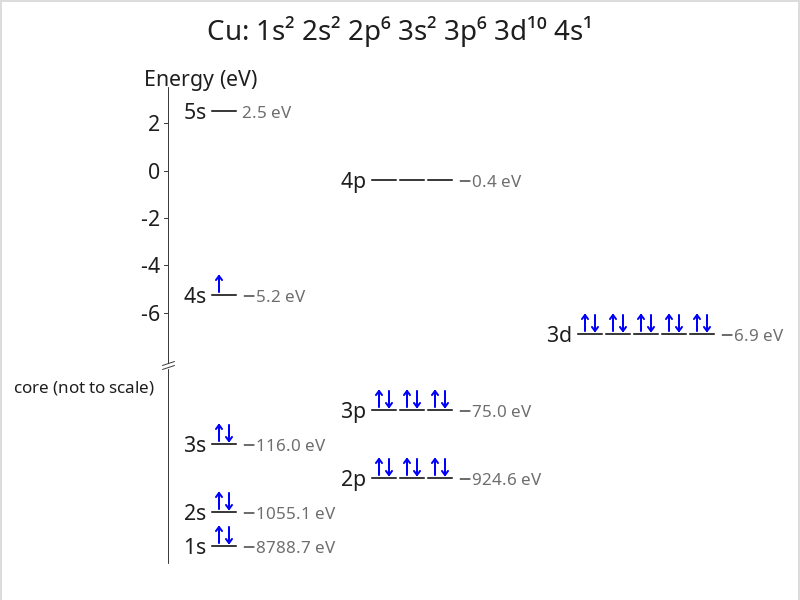
\includegraphics[width=0.8\linewidth]{periodic-trends/tm-mo-cu.ecce-9.5.3-dev.png}
	\caption{The \menu{MO Diagram} panel of copper (B3LYP), energies to scale, with the core below the axis break. The filled 3d level lies below the singly occupied 4s.}
	\label{fig:pt-tm}
\end{figure}

Do not teach the exceptions from this figure. Orbital energies do not decide the configuration; total energies do, and 3d$^4$4s$^2$ chromium or 3d$^9$4s$^2$ copper would each be a separate calculation. The topic has only the observed configurations, so it cannot show that they are the lower ones. The empty orbitals of calcium depend on the basis set, so their order is not to be taught either. \XXX[ check whether ECCE-QM can hold copper in 3d$^9$4s$^2$.]
\index{Exceptions to the Aufbau order}\index{Aufbau principle!exceptions}

\section{Effective nuclear charge}
\index{Effective nuclear charge!from orbital energies}
We take the energy of the highest occupied orbital from the \menu{MOs} panel of the Hartree-Fock calculations in \menu{Koopmans' theorem}, where the column \menu{E (Hartree)} gives it in the unit that equation~\eqref{eq:zeff} needs. For lithium the 2s orbital of \menu{Li\_HF} lies at $-0.1964$~hartree, so that
\begin{equation*}
	Z_\mathrm{eff} = 2\sqrt{2 \times 0.1964} = 2\sqrt{0.3928} = 1.25 ,
\end{equation*}
and for neon the 2p orbitals of \menu{Ne\_HF} lie at $-0.8512$~hartree, which gives $Z_\mathrm{eff} = 2\sqrt{1.7024} = 2.61$. For the third period $n = 3$: the 3s orbital of sodium at $-0.1822$~hartree gives $3\sqrt{0.3644} = 1.81$. Figure~\ref{fig:pt-zeff} shows the same calculation for every atom from H to Ar. Across a period it rises by about 0.3 per element, from 1.25 (Li) to 2.61 (Ne) and from 1.81 (Na) to 3.26 (Ar), because each added proton is only partly screened by the electron added with it. It falls back at each alkali metal, where a new shell starts. The breaks at B, Al, O and S are the same as in the ionisation energies, since this $Z_\mathrm{eff}$ is the Koopmans IE in other units.

\begin{figure}[htbp]
	\centering
	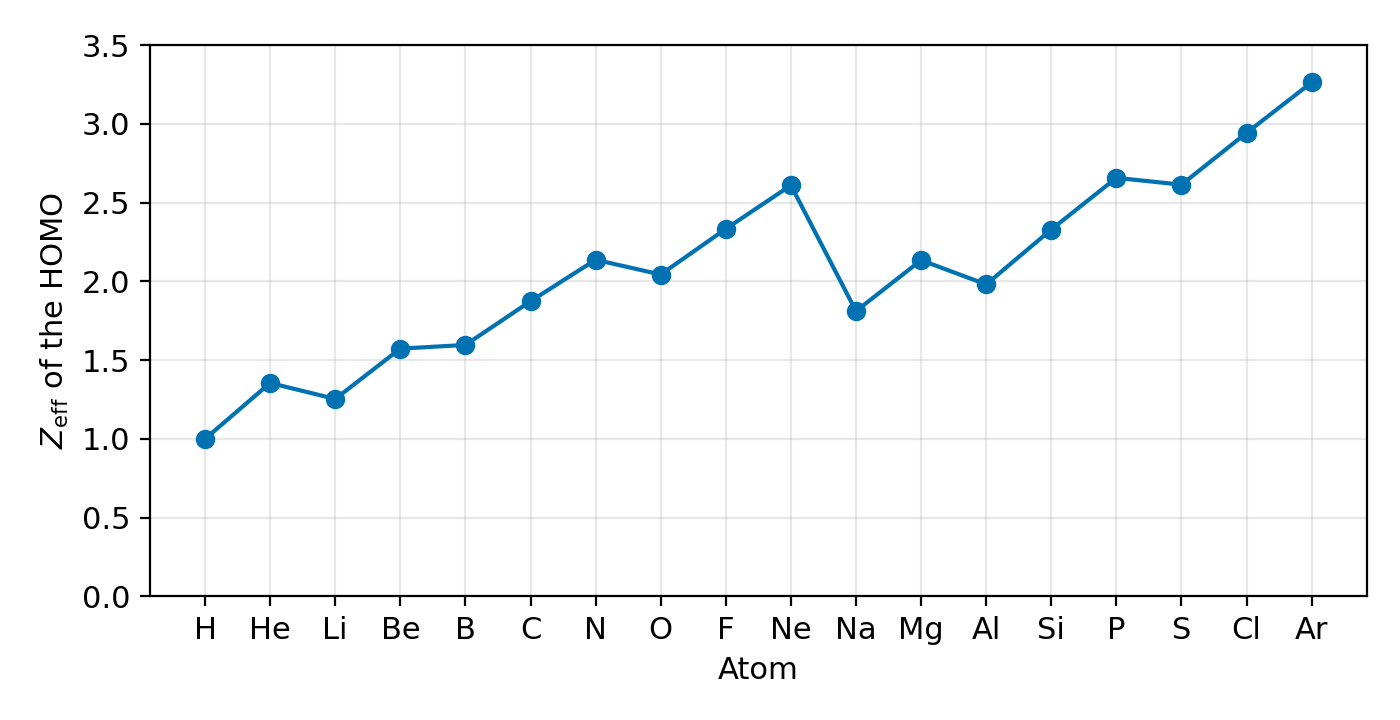
\includegraphics[width=0.85\linewidth]{periodic-trends/zeff.ecce-9.5.2-dev.png}
	\caption{Effective nuclear charge of the highest occupied orbital from equation~\eqref{eq:zeff} and Hartree-Fock/aug-cc-pVTZ orbital energies, plotted from the values in the \menu{MOs} panel.}
	\label{fig:pt-zeff}
\end{figure}

\index{Slater's rules}
For one electron outside a closed shell the estimate agrees with Slater's rules: 1.25 against 1.30 for lithium. For a full shell it does not: Slater gives 5.85 for the 2p of neon, equation~\eqref{eq:zeff} 2.61. The difference is the repulsion with the other seven $n = 2$ electrons, which the orbital energy contains. Teach the trend across a period; the absolute values depend on the definition.

\section{First ionisation energies}
\index{Ionisation energy!across a period}\index{Periodic trends!ionisation energy}\index{Comparing with experiment}
Table~\ref{tab:pt-ie} and figure~\ref{fig:pt-ie} compare the calculated values with experiment \cite{nistasd}. Koopmans' values show the whole textbook curve: the rise across a period, the maxima at the noble gases, the drops to Li and Na, the dips at O, S and Al. Hydrogen gives 13.60~eV, as it must for one electron.

\begin{table}[htb]
	\centering\small
	\caption{First ionisation energies in eV. Koopmans: $-\varepsilon_\mathrm{HOMO}$, Hartree-Fock/aug-cc-pVTZ. $\Delta$SCF: $E(\mathrm{A}^+) - E(\mathrm{A})$, Hartree-Fock/aug-cc-pVTZ. B3LYP: $-\varepsilon_\mathrm{HOMO}$. Experiment: NIST ASD \cite{nistasd}.}
	\label{tab:pt-ie}
	\begin{tabular}{l rrrr}
		\hline
		Atom & Koopmans & $\Delta$SCF & B3LYP & Experiment \\
		\hline
		H  & 13.60 &       &  8.68 & 13.60 \\
		He & 24.98 &       & 17.90 & 24.59 \\
		Li &  5.34 &  5.34 &  3.57 &  5.39 \\
		Be &  8.42 &  8.04 &  6.24 &  9.32 \\
		B  &  8.67 &       &  5.03 &  8.30 \\
		C  & 11.94 & 10.80 &  7.22 & 11.26 \\
		N  & 15.53 & 13.90 &  9.67 & 14.53 \\
		O  & 14.20 & 12.03 &  9.85 & 13.62 \\
		F  & 18.51 & 15.67 & 12.63 & 17.42 \\
		Ne & 23.16 & 19.69 & 15.57 & 21.56 \\
		Na &  4.96 &       &  3.41 &  5.14 \\
		Mg &  6.89 &       &  5.21 &  7.65 \\
		Al &  5.93 &       &  3.51 &  5.99 \\
		Si &  8.20 &       &  5.19 &  8.15 \\
		P  & 10.67 &       &  7.04 & 10.49 \\
		S  & 10.32 &       &  7.46 & 10.36 \\
		Cl & 13.09 &       &  9.47 & 12.97 \\
		Ar & 16.09 &       & 11.59 & 15.76 \\
		\hline
	\end{tabular}
\end{table}

\begin{figure}[htbp]
	\centering
	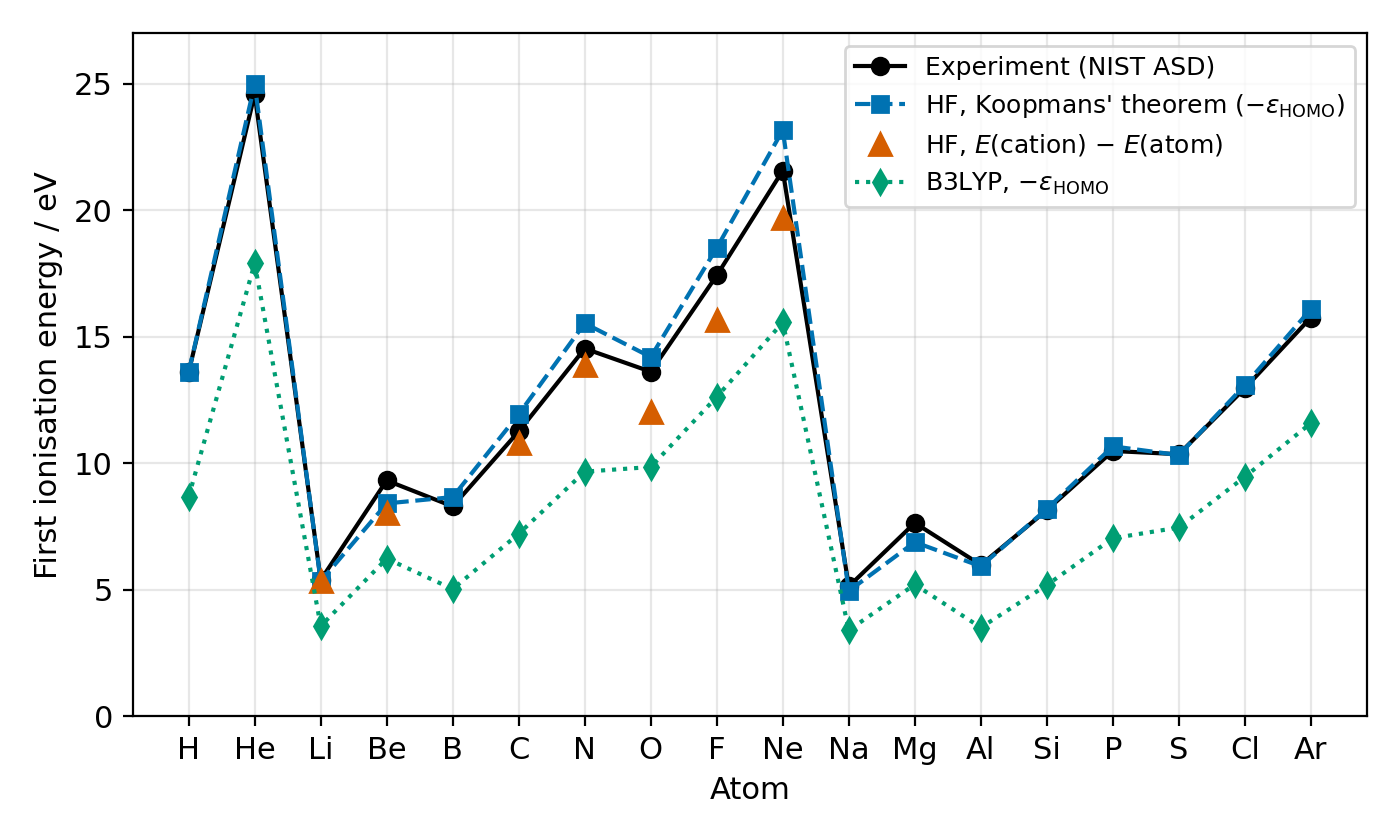
\includegraphics[width=\linewidth]{periodic-trends/ie.ecce-9.5.2-dev.png}
	\caption{First ionisation energies of H to Ar. Black: experiment \cite{nistasd}. Blue: Koopmans. Orange: $\Delta$SCF. Green: $-\varepsilon_\mathrm{HOMO}$ from B3LYP.}
	\label{fig:pt-ie}
\end{figure}

\index{Koopmans' theorem!errors}\index{Relaxation}
$\Delta$SCF is below experiment for all seven atoms, by 0.05~eV at Li and 1.6 to 1.9~eV at O, F and Ne: the missing correlation. Koopmans' values lie above $\Delta$SCF by the relaxation energy (1.1~eV for C, 3.5~eV for Ne). The two errors partly cancel, which is why Koopmans' theorem looks good in figure~\ref{fig:pt-ie}. Do not present it as the more accurate method. For lithium the relaxation is negligible: the Koopmans value, $0.1964~\text{hartree} = 5.344$~eV, and $\Delta$SCF, 5.342~eV from the Energy Calculator, agree to 0.002~eV, because removing the outer electron hardly changes the core.

\index{B3LYP!orbital energies}\index{Density functional theory!HOMO energy}
The B3LYP orbital energies follow the same pattern a few eV lower (8.68~eV for hydrogen). With a density functional, take ionisation energies from total energies, not orbital energies.

\section{The dips at boron and oxygen}
\label{sec:pt-dips}
\index{Ionisation energy!dip at boron}\index{Ionisation energy!dip at oxygen}\index{Boron}\index{Aluminium}\index{Sulfur}
The measured IE falls from Be to B, from N to O, and again from Mg to Al and from P to S. At B and Al the electron removed is the first p electron, which penetrates less than an s electron. At O and S it is the first electron to pair in a p orbital.

\index{Pairing energy}\index{Electron pairing}
The unrestricted Hartree-Fock calculations show the pairing directly. In nitrogen the three alpha 2p orbitals lie at $-0.571$~hartree and there is no beta 2p electron. In oxygen the fourth 2p electron is beta, paired in an orbital with an alpha electron, and lies at $-0.522$~hartree, above all the alpha 2p orbitals. Koopmans gives 14.20~eV for oxygen against 15.53~eV for nitrogen. $\Delta$SCF drops by 1.87~eV, twice the measured 0.92~eV (from the unrounded values 14.534 and 13.618~eV), since Hartree-Fock misses more correlation in oxygen, which has one more electron pair. The cations confirm the counts: O$^+$ is a quartet, N$^+$ a triplet.

\index{Koopmans' theorem!failure for beryllium}\index{Beryllium}
At boron Koopmans' theorem fails: its values \emph{rise} from Be to B (8.42 to 8.67~eV) where experiment falls. Beryllium is 0.90~eV too low, because its 2s$^2$ pair mixes strongly with the nearby empty 2p, a correlation Hartree-Fock omits. Between Mg and Al the gap is wide enough that Koopmans' values fall (6.89 to 5.93~eV). Show the s-to-p dip in the third period.

\section{Electron affinities}
\index{Electron affinity!across a period}\index{Anions}
Table~\ref{tab:pt-ea} gives the electron affinities from PBE0/aug-cc-pVDZ. Fluorine takes up an electron most readily (3.29~eV), filling its 2p. Carbon and oxygen give about 1.4~eV, lithium 0.49~eV. Beryllium and nitrogen come out negative: the anion is higher than the atom. In beryllium the new electron has to go into 2p; in nitrogen it has to pair. These are the same two effects as in the IE dips.

\begin{table}[htb]
	\centering\small
	\caption{Electron affinities, $E(\mathrm{A}) - E(\mathrm{A}^-)$, PBE0/aug-cc-pVDZ, with the multiplicities of atom and anion.}
	\label{tab:pt-ea}
	\begin{tabular}{l cc rr r}
		\hline
		Atom & $2S+1$ atom & $2S+1$ anion & EA / eV & EA / kJ\,mol$^{-1}$ & Experiment / eV \\
		\hline
		Li & 2 & 1 &  0.49 &  47.4 & \XXX \\
		Be & 1 & 2 & $-0.04$ & $-3.8$ & \XXX \\
		C  & 3 & 4 &  1.41 & 136.5 & \XXX \\
		N  & 4 & 3 & $-0.12$ & $-11.7$ & \XXX \\
		O  & 3 & 2 &  1.39 & 134.5 & \XXX \\
		F  & 2 & 1 &  3.29 & 317.6 & \XXX \\
		\hline
	\end{tabular}
\end{table}

\index{Electron affinity!negative}
A negative EA in a finite basis set is only an indication: an unbound anion has no stable state, and its computed energy depends on the basis set. Teach the sign, not the size. Never read an EA from the anion's orbital energies: the HOMO of Li$^-$ and C$^-$ lies above zero, although both anions are bound by total energy.

\section{History}
\index{History!Koopmans}\index{History!Slater}\index{History!Hund}
Slater published his screening rules in 1930 \cite{slater1930}, Koopmans his theorem in 1934 \cite{koopmans1934}. Hund's rules came from his analysis of atomic spectra \XXX[ citation and year].

\chapter{Polar covalent and ionic bonds}
\label{ch:t-polar-ionic}
\index{Polar bond}
\index{Ionic bond}
\index{Dipole moment}
\index{Localised orbitals}
\eccexample{Examples > General Chemistry > Polar bonds and dipole moments}

A textbook draws \chem{H2} with a shared electron pair, \chem{NaCl} as two ions and \chem{HF} somewhere in between, and students ask where the line between a covalent and an ionic bond lies. This chapter gives the teacher one number for each of six molecules that answers the question on the board: how much charge has moved from one atom to the other, worked out from the dipole moment and the bond length. The numbers show that the charge separation grows step by step from \chem{HBr} to \chem{NaCl}, with no jump, and the localised orbitals of \chem{HF} and \chem{LiF} show where a chemist stops drawing a bond between the two atoms.

\section*{This requires}
Nothing beyond ECCE: the calculations are in the General Chemistry example set.

\section{The calculations}
Six stored calculations of single molecules in the gas phase are used. \emph{HF\_dipole}, \emph{HCl} and \emph{HBr} are in the topic \menu{Polar bonds and dipole moments}, \emph{LiH} and \emph{LiF} in \menu{Molecular orbitals of diatomics}, and \emph{nacl\_ion\_pair} in \menu{Intermolecular interactions}. Each is an optimised structure, so the bond length is the one the calculation finds for the molecule at rest.
\XXX[LiF: the stored optimisation stopped after 100 steps without meeting its convergence criteria (bond length steady at 1.554~\AA, no frequencies). Rerun before release; the numbers below are from the last step.]

\section{Procedure}
\begin{enumerate}
	\item In the Organizer, choose \menu{File > Open Example Calculations}, pick \menu{General Chemistry} and click \menu{OK}.
	\item Open \emph{HF\_dipole} in the Viewer. With \menu{Measure} (Chapter~\ref{ch:first-calculation}), measure the H--F distance.
	\item Open \menu{Properties > Electric properties > Dipole Moment} and read the total dipole moment in debye.
	\item Repeat for \emph{HCl}, \emph{HBr}, \emph{LiH}, \emph{LiF} and \emph{nacl\_ion\_pair}.
	\item In \emph{HF\_dipole} and \emph{LiF}, open \menu{Properties > Orbitals > MOs}, choose \menu{Localised MO} in the box next to \menu{Compute}, and read the \menu{Bond type} column.
\end{enumerate}
\index{Dipole moment!showing}

\section{How much charge has moved}
A dipole moment $\mu$ is a charge $q$ times the distance $R$ that separates it from an equal and opposite charge, $\mu = qR$. If one whole electron had moved from one atom to the other, the dipole moment would be $eR$; with $R$ in \AA{} and $\mu$ in debye (D, the unit in which dipole moments are tabulated) that is $4.803\,R$~D. Dividing the dipole moment by this value gives the fraction of an electron that has moved, $q/e = \mu/(4.803\,R)$: 0 for a bond shared equally, 1 for two whole ions. This number needs only the dipole moment and the bond length, and both can be measured, so calculation and experiment can be put side by side (table~\ref{tab:pi-q}).

\begin{table}[htbp]
	\centering
	\caption{Bond length $R$, dipole moment $\mu$ and the fraction of an electron moved, $q/e=\mu/(4.803\,R)$, for six molecules in the gas phase. Calculated values from the stored ECCE calculations; measured bond lengths from the NIST Chemistry WebBook \cite{nistwebbook}, measured dipole moments from the NIST CCCBDB \cite{cccbdb}.}
	\label{tab:pi-q}
	\begin{tabular}{lrrrrrr}
		\toprule
		& \multicolumn{3}{c}{calculated} & \multicolumn{3}{c}{measured} \\
		\cmidrule(lr){2-4}\cmidrule(lr){5-7}
		Molecule & $R$ (\AA) & $\mu$ (D) & $q/e$ & $R$ (\AA) & $\mu$ (D) & $q/e$ \\
		\midrule
		\chem{HBr}  & 1.428 & 1.01 & 0.15 &       & 0.83 & \\
		\chem{HCl}  & 1.290 & 1.47 & 0.24 &       & 1.09 & \\
		\chem{HF}   & 0.935 & 1.86 & 0.42 & 0.917 & 1.83 & 0.42 \\
		\chem{LiH}  & 1.622 & 5.63 & 0.72 &       & 5.88 & \\
		\chem{LiF}  & 1.554 & 5.58 & 0.75 & 1.564 & 6.28 & 0.84 \\
		\chem{NaCl} & 2.364 & 8.59 & 0.76 & 2.361 & 8.97 & 0.79 \\
		\bottomrule
	\end{tabular}
\end{table}

The table shows that the charge separation rises steadily down the list, from 0.15 of an electron in \chem{HBr} to about 0.8 in \chem{LiF} and \chem{NaCl}, because the difference in electronegativity between the two atoms grows down the list. Hence no molecule marks the point where a bond suddenly turns ionic; polar covalent and ionic are the two ends of one scale. The measured values say the same: \chem{HF} moves 0.42 of an electron in both columns, and \chem{LiF} and \chem{NaCl} come out at 0.84 and 0.79. Even in \chem{NaCl}, the textbook ionic compound, the measured dipole moment is only 79\,\% of what two whole charges would give, because the positive sodium ion pulls the electron cloud of the chloride ion a little back toward itself.

The calculated dipole moments of \chem{HCl} and \chem{HBr} are a quarter to a third larger than the measured ones, and those of \chem{LiH}, \chem{LiF} and \chem{NaCl} a little smaller, so for these molecules the table is best read for its order, which is the same in both columns.

\section{Where a chemist stops drawing a bond}
The localised orbitals of the procedure divide the electrons of a molecule into cores, bonds and lone pairs, the pieces of a Lewis structure. In \chem{HF} one of the four valence electron pairs is listed as \texttt{sigma H1-F2}, a pair shared between the two atoms, and the other three as lone pairs on fluorine. In \chem{LiF} all four valence pairs are listed as lone pairs on fluorine and none as a bond. This shows that the pair that \chem{HF} shares with hydrogen has become, in \chem{LiF}, a fourth lone pair of a fluoride ion, because lithium holds its valence electron far less tightly than hydrogen does. Hence the orbitals switch from ``bond'' to ``ion pair'' somewhere between 0.42 and 0.75 of an electron moved, while the dipole moment changes smoothly: Li$^+$F$^-$ is the better Lewis structure for \chem{LiF}, and H--F the better one for \chem{HF}.
\index{Lewis structure}

\section{In class}
Write the six molecules on the board in the order of the table and ask the class where to draw the line between covalent and ionic. The fraction $q/e$ then shows that any line is a choice, and the localised orbitals show where the usual choice puts it.

\section{History}
Debye introduced the permanent dipole moment of a molecule in 1912 \cite{debye1912}. Pauling built his electronegativity scale in 1932 from the extra energy of a bond between two unlike atoms over the mean of the two like bonds \cite{pauling1932}; the larger the difference in electronegativity, the more ionic the bond.
\index{Debye, Peter}\index{Pauling, Linus}

\chapter{Resonance}
\label{ch:t-resonance}
\XXX[to be written: ozone, nitrate, the carboxylate: one structure with delocalised orbitals, equal bond lengths]

\chapter{Molecular shapes from electron domains}
\label{ch:t-shapes}
\XXX[to be written: four, five and six domains: CH4, NH3, H2O, PF5, SF4, ClF3, SF6; isomers that relax to the same shape]

\chapter{Molecular dipole moments}
\label{ch:t-dipoles}
\index{Dipole moment}
\index{Bond dipole}
\index{Carbon dioxide}\index{Sulfur dioxide}\index{Water}
\eccexample{Examples > General Chemistry > Polar bonds and dipole moments}

Students learn that a molecule with polar bonds can still be non-polar, and that the shape decides. This chapter gives the teacher the numbers to show it: the charges on the atoms, which say how polar each bond is, next to the dipole moment of the whole molecule, which says whether the bond dipoles cancel. \chem{CO2} and \chem{SO2} make the central pair, two molecules with the same kind of bonds, one linear and one bent, and \chem{BF3}, \chem{CH4} and \chem{SF6} show the same cancellation in three dimensions.

\section*{This requires}
Nothing beyond ECCE: the calculations are in the General Chemistry example set.

\section{The calculations}
All eight molecules are in the topic \menu{Polar bonds and dipole moments}: \emph{CO2}, \emph{SO2}, \emph{CH3F}, \emph{H2O\_dipole}, \emph{NH3\_dipole}, \emph{BF3\_dipole}, \emph{CH4\_dipole} and \emph{SF6\_dipole}. Each is a single molecule in the gas phase at its optimised structure, and all were calculated in the same way, with a basis set chosen to give good dipole moments.

\section{Procedure}
\begin{enumerate}
	\item In the Organizer, choose \menu{File > Open Example Calculations}, pick \menu{General Chemistry} and click \menu{OK}.
	\item Open \emph{CO2} in the Viewer. Open \menu{Properties > Charges > CHELPG / ESP-Fitted Charges} to see the charge on each atom, and \menu{Properties > Electric properties > Dipole Moment} for the dipole moment of the molecule.
	\item With \menu{Measure} (Chapter~\ref{ch:first-calculation}), measure the angle O--C--O.
	\item Repeat for \emph{SO2} (angle O--S--O), \emph{H2O\_dipole} (H--O--H), \emph{NH3\_dipole}, \emph{CH3F}, \emph{BF3\_dipole}, \emph{CH4\_dipole} and \emph{SF6\_dipole}.
	\item In \emph{CO2}, \emph{SO2} and \emph{H2O\_dipole}, open \menu{Properties > Orbitals > MOs}, choose \menu{ESP on Density} in the box next to \menu{Compute} and click \menu{Compute}.
\end{enumerate}
\index{Dipole moment!showing}\index{Charges!ESP-fitted}

\section{Polar bonds, polar molecules}
The charges are the ones that best reproduce the electric field the calculated molecule produces around itself, so they say how the molecule looks to a neighbouring charge; a positive number means the atom has given up part of an electron. The dipole moment is in debye (D): one debye is about a fifth of the dipole of one electron and one proton \SI{1}{\angstrom} apart.

\begin{table}[htbp]
	\centering
	\caption{Charge on the central atom (in units of the proton charge), bond angle and dipole moment $\mu$ of eight molecules. Calculated values from the stored ECCE calculations; measured dipole moments in the gas phase from the NIST CCCBDB \cite{cccbdb}. A dash means the molecule's symmetry makes the dipole moment exactly zero.}
	\label{tab:dp}
	\begin{tabular}{lrrrr}
		\toprule
		Molecule & central atom charge & angle & $\mu$ calc.\ (D) & $\mu$ meas.\ (D) \\
		\midrule
		\chem{CO2} & C $+0.78$ & \ang{180} & 0 & -- \\
		\chem{BF3} & B $+0.91$ & \ang{120} & 0 & -- \\
		\chem{CH4} & C $-0.32$ & \ang{109.5} & 0 & -- \\
		\chem{SF6} & S $+0.59$ & \ang{90} & 0 & -- \\
		\chem{SO2} & S $+0.59$ & \ang{117.5} & 1.92 & 1.63 \\
		\chem{H2O} & O $-0.67$ & \ang{104.7} & 1.85 & 1.86 \\
		\chem{NH3} & N $-0.85$ & \ang{106.8} & 1.52 & 1.48 \\
		\chem{CH3F} & F $-0.26$ & & 1.91 & 1.85 \\
		\bottomrule
	\end{tabular}
\end{table}

Table~\ref{tab:dp} shows that the first four molecules have strongly charged central atoms and still no dipole moment, because their bonds point symmetrically in opposite directions and the bond dipoles cancel. In \chem{CO2} the carbon carries $+0.78$ and each oxygen $-0.39$, so each C=O bond is clearly polar, but the two bonds point away from carbon along one line, and the two bond dipoles, equal in size and opposite in direction, add up to zero. In \chem{BF3} three bond dipoles at \ang{120} cancel in the plane, and in \chem{CH4} and \chem{SF6} four and six cancel in space. Hence a molecule is non-polar whenever its polar bonds are arranged so that the centre of the negative charge falls on the centre of the positive charge.

\chem{SO2} has the same kind of bonds as \chem{CO2}, sulfur positive and oxygen negative, but it is bent at \ang{117.5}, and its dipole moment is 1.92~D (measured 1.63~D). The two bond dipoles now point partly the same way, toward the side of the oxygen atoms, and no longer cancel. Hence the shape, and not the bonds alone, decides whether a molecule is polar; why \chem{SO2} is bent and \chem{CO2} is not is the subject of Chapter~\ref{ch:t-shapes}.

\section{Where the dipole moment comes from}
The dipole moment that ECCE shows is worked out from the whole charge of the molecule: each nucleus is a positive point charge at its position, and the electrons are a cloud of negative charge spread over the molecule, the electron density of the calculation. Each piece of charge is multiplied by its position and all of them are added up. For a neutral molecule the result does not depend on where the positions are measured from, and it is zero exactly when the centre of the positive charge and the centre of the negative charge fall on the same point. In physics the dipole points from the centre of negative charge to the centre of positive charge; chemists usually draw the arrow the other way, towards the negative end, as in the figures of this chapter.
\index{Dipole moment!how it is calculated}

Bond dipoles are a way of splitting this one vector into pieces a class can draw. Give each atom its charge from the table and take the outer atom of each bond: its charge times the bond, as an arrow along the bond, is that bond's dipole. Added as arrows, head to tail, the bond dipoles of a neutral molecule give exactly the dipole of the atomic charges, and that is close to the dipole moment worked out from the whole charge cloud: for water 1.90~D against 1.85~D.

\begin{figure}[htbp]
	\centering
	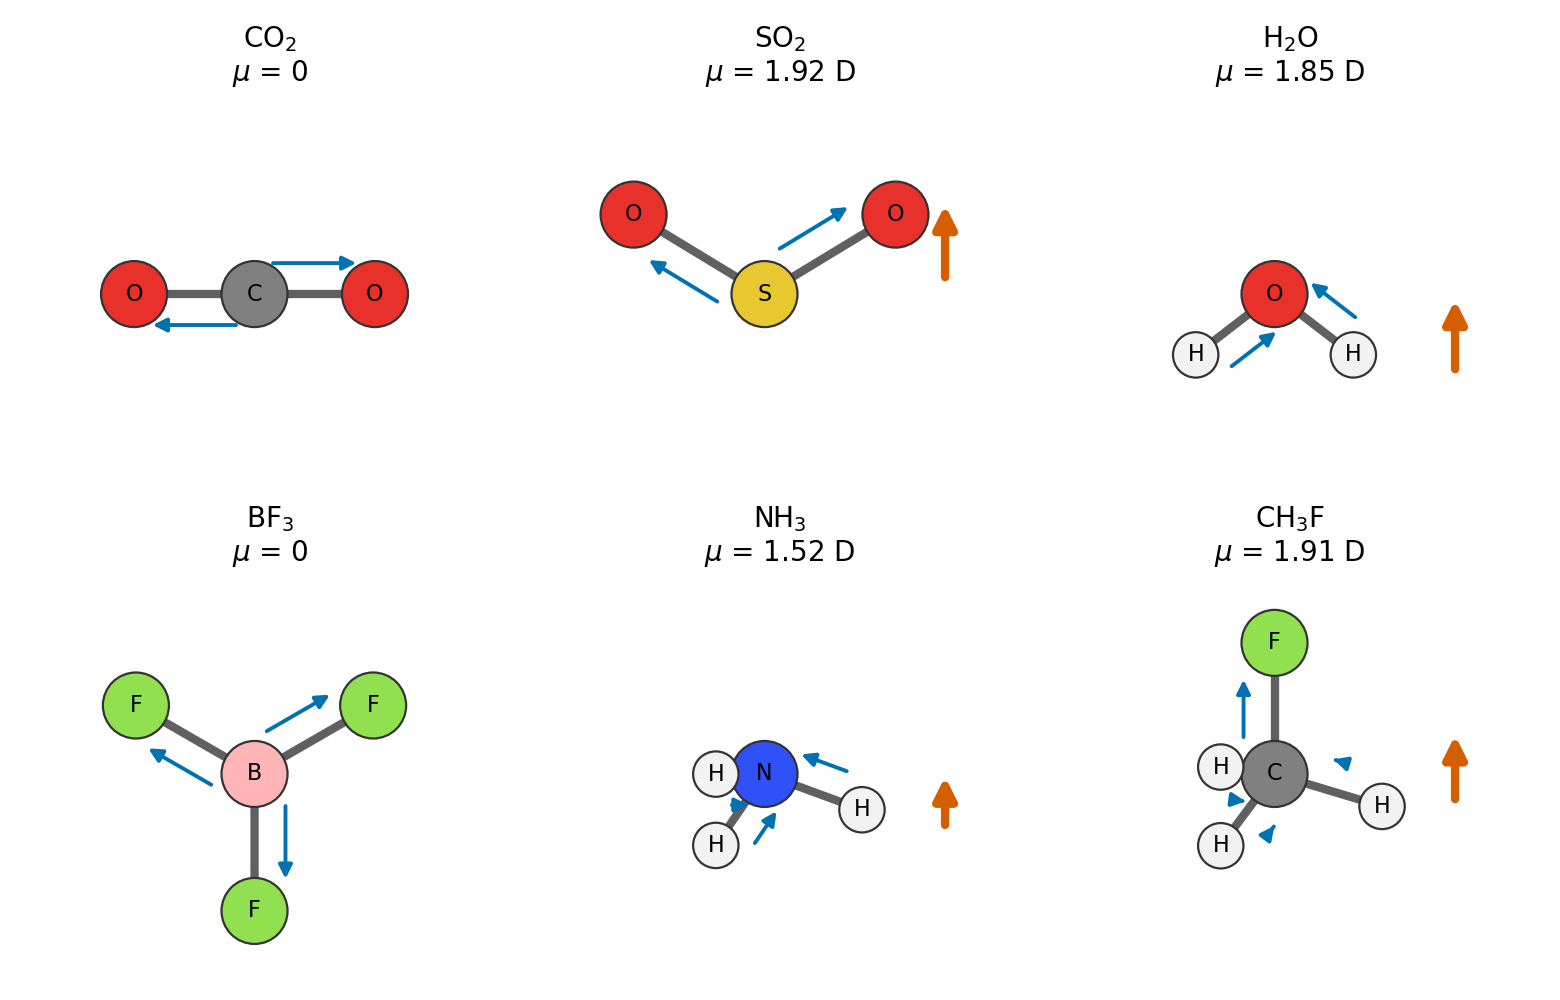
\includegraphics[width=0.95\linewidth]{dipoles/bond-dipoles.ecce-9.5.3-dev.png}
	\caption{Bond dipoles (thin blue arrows, one beside each bond) and the dipole moment of the whole molecule (thick orange arrow, drawn beside the molecule) of six of the molecules of table~\ref{tab:dp}, all pointing towards the negative end. Each bond dipole is the charge of its outer atom times the bond, from the stored atomic charges; the molecular dipole is the calculated dipole moment, at the same scale. \chem{NH3} and \chem{CH3F} are seen from a little above, so that all their atoms show. Drawn from the stored ECCE results.}
	\label{fig:dp-arrows}
\end{figure}

Figure~\ref{fig:dp-arrows} shows the bond dipoles of \chem{CO2} pointing away from each other along one line and those of \chem{BF3} pointing to the corners of a triangle, while those of \chem{SO2}, \chem{H2O}, \chem{NH3} and \chem{CH3F} all lean towards one side of the molecule. This is because the arrows add head to tail: two equal arrows in opposite directions, or three at \ang{120}, end where they started, while arrows that share a direction leave a sum. Hence the thick arrow appears only on the bent and pyramidal molecules and on \chem{CH3F}, whose one strong C--F bond dipole is not balanced by the three weak C--H ones.

\begin{figure}[htbp]
	\centering
	\begin{tabular}{ccc}
		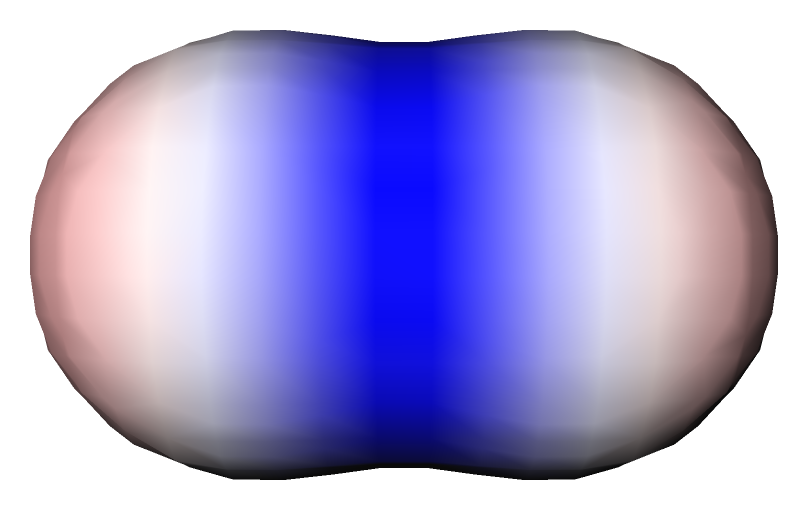
\includegraphics[height=2.6cm]{dipoles/co2-esp.ecce-9.5.3-dev.png} &
		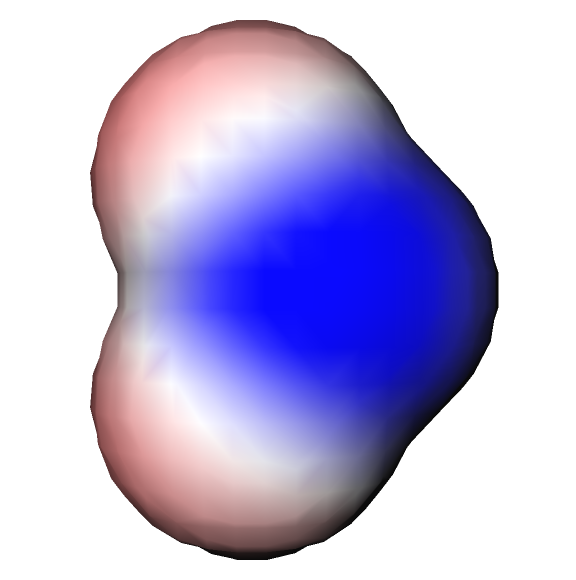
\includegraphics[height=2.6cm]{dipoles/so2-esp.ecce-9.5.3-dev.png} &
		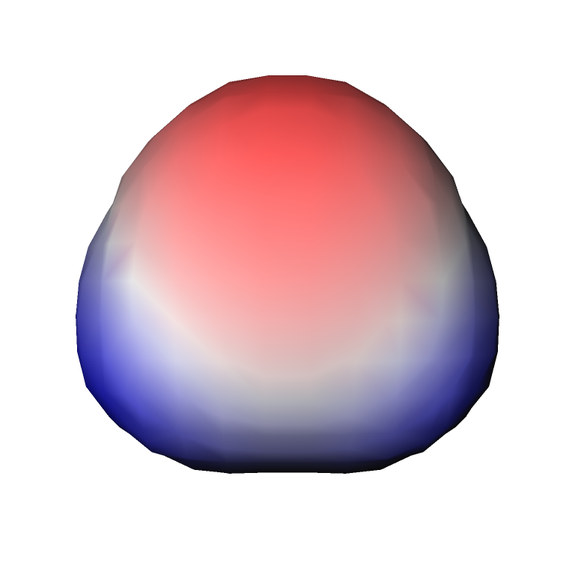
\includegraphics[height=2.6cm]{dipoles/h2o-esp.ecce-9.5.3-dev.png} \\
		\chem{CO2} & \chem{SO2} & \chem{H2O} \\
	\end{tabular}
	\caption{The electric potential on a surface of constant electron density (\menu{ESP on Density} in the \menu{MOs} panel), red negative and blue positive, each picture on its own colour scale (\menu{ESP range: Auto}). \chem{CO2}: the O atoms at the left and right ends, C in the middle. \chem{SO2}: the two O atoms on the left, S on the right. \chem{H2O}: O at the top, the two H atoms at the lower corners.}
	\label{fig:dp-esp}
\end{figure}

Figure~\ref{fig:dp-esp} shows where the charge sits on the outside of each molecule. \chem{CO2} is red at both ends and blue round the middle, symmetric front to back, while \chem{SO2} and \chem{H2O} are red on one side and blue on the other, because a straight molecule puts its negative oxygen atoms at the two ends and a bent one puts them on the same side. Hence a molecule with one red side and one blue side has a dipole moment, and a molecule whose colours are arranged symmetrically has none, which a class can judge from the picture before reading the number.

\section{Adding bond dipoles}
For a bent molecule with two equal bonds the addition can be done on the board. Each bond dipole $\mu_\mathrm{b}$ points along its bond; the components across the molecule cancel and the components along the axis add, so $\mu = 2\mu_\mathrm{b}\cos(\theta/2)$, where $\theta$ is the bond angle. With the calculated values, water ($\mu = 1.85$~D, $\theta = \ang{104.7}$) has a bond dipole of 1.52~D per O--H bond, and \chem{SO2} ($\mu = 1.92$~D, $\theta = \ang{117.5}$) one of 1.85~D per S=O bond. This shows that the bond dipoles of the two molecules are of a similar size, because both bonds join an electronegative atom to a less electronegative one. Hence the angle decides most of the difference between bent and straight molecules: the factor $\cos(\theta/2)$ is 0.61 at \ang{104.7}, 0.52 at \ang{117.5}, and at \ang{180}, the angle of \chem{CO2}, it is zero.
\index{Bond dipole!addition}

The calculated dipole moments of \chem{H2O}, \chem{NH3} and \chem{CH3F} are within 3\,\% of the measured ones; that of \chem{SO2} is 18\,\% too large, so in the calculated column \chem{SO2} comes out as the most polar of the four, while measured it is third. The zeros of the symmetric molecules and the contrast between \chem{CO2} and \chem{SO2} hold exactly in both columns; to rank the four polar molecules, use the measured one.

\section{In class}
Show \chem{CO2} and \chem{SO2} side by side with their charges switched on or their ESP surfaces drawn, ask whether each molecule is polar, and then show the dipole moments. Draw the two bond dipoles as arrows on each molecule; the class can see that the arrows of \chem{CO2} point away from each other along one line and those of \chem{SO2} add up.

\section{History}
Debye introduced the permanent dipole moment of a molecule in 1912 to explain how the dielectric constant of a substance depends on temperature \cite{debye1912}, and collected the theory and the measured values in his book \emph{Polar Molecules} of 1929 \cite{debye1929}.
\index{Debye, Peter}

\chapter{Electron domains and hybridisation}
\label{ch:t-hybridisation}
\XXX[to be written: what the orbitals of methane, ethene and ethyne look like, and what hybridisation describes]

\chapter{The chemical bond in \chem{H2}}
\label{ch:t-h2-bond}
\XXX[to be written: the potential curve, bond length and dissociation energy; restricted and unrestricted at long distance]

\chapter{Bonds, antibonds and bond order}
\label{ch:t-bond-order}
\index{Bond order}
\index{Antibonding orbital}
\index{Hydrogen molecule}\index{Helium dimer}
\eccexample{Examples > General Chemistry > Molecular orbitals of diatomics}

Molecular orbital theory explains why two hydrogen atoms form a molecule and two helium atoms do not with one rule: electrons in a bonding orbital hold the atoms together, electrons in an antibonding orbital push them apart, and the bond order is half the difference. This chapter gives the teacher four molecules that make the rule concrete, \chem{H2+}, \chem{H2}, \chem{He2+} and \chem{He2}, with bond orders \textonehalf, 1, \textonehalf{} and 0, and shows a class that the bond order predicts which bonds are shortest and stiffest, and that \chem{He2} has no bond at all.

\section*{This requires}
Nothing beyond ECCE: the calculations are in the General Chemistry example set.

\section{The calculations}
The topic \menu{Molecular orbitals of diatomics} holds \emph{H2\_cation}, \emph{H2}, \emph{He2\_cation} and \emph{He2}. The first three are optimised structures with their vibrational frequencies. \emph{He2} cannot be optimised, because the two atoms do not bind; it is a single calculation with the atoms held \SI{3.0}{\angstrom} apart.

\section{Procedure}
\begin{enumerate}
	\item In the Organizer, choose \menu{File > Open Example Calculations}, pick \menu{General Chemistry} and click \menu{OK}.
	\item Open \emph{H2} in the Viewer and choose \menu{Properties > Orbitals > MOs}. Note which orbitals are occupied and draw the lowest occupied and the lowest empty orbital with \menu{Compute}.
	\item With \menu{Measure} (Chapter~\ref{ch:first-calculation}), measure the H--H distance, and open \menu{Properties > Vibrational spectra > Vibrational Frequencies} for the stretching frequency.
	\item Repeat for \emph{H2\_cation}, \emph{He2\_cation} and \emph{He2} (\emph{He2} has no frequencies).
\end{enumerate}
\index{MOs panel}

\section{Bond order}
Two 1s orbitals combine into two molecular orbitals: $\sigma$, with the electron density gathered between the nuclei, and $\sigma^*$, with a node half way between them. Filling the orbitals from the bottom gives table~\ref{tab:bo}: \chem{H2+} has one electron in $\sigma$, \chem{H2} two, \chem{He2+} two in $\sigma$ and one in $\sigma^*$, and \chem{He2} two in each. The bond order is (bonding electrons $-$ antibonding electrons)/2.

\begin{figure}[htbp]
	\centering
	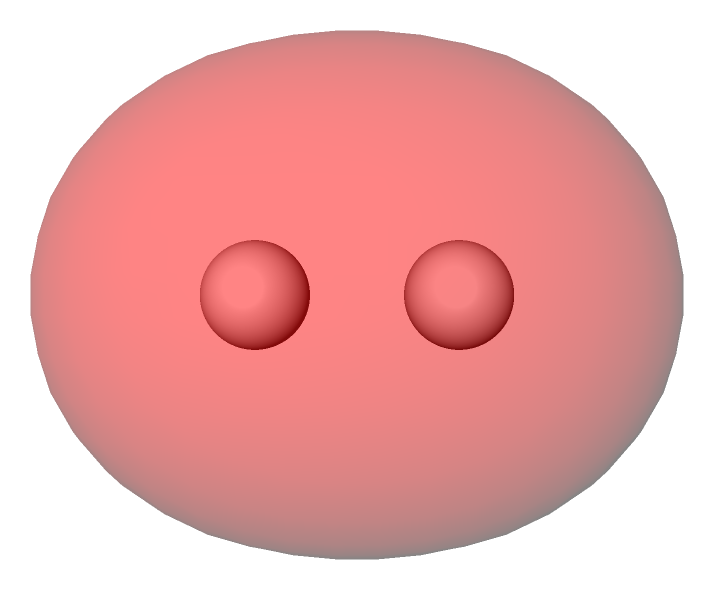
\includegraphics[width=0.3\linewidth]{bond-order/h2-sigma.ecce-9.5.3-dev.png}\hspace{4mm}
	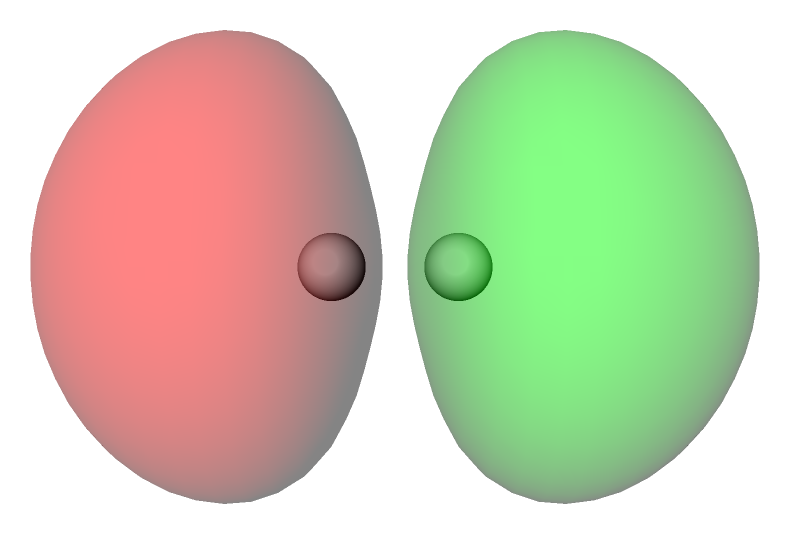
\includegraphics[width=0.3\linewidth]{bond-order/h2-sigmastar.ecce-9.5.3-dev.png}\\[3mm]
	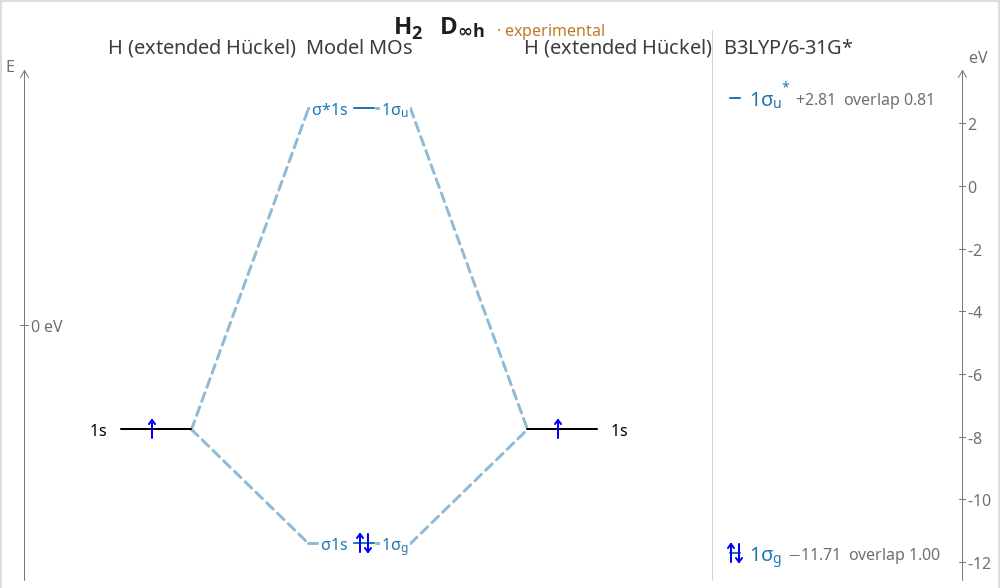
\includegraphics[width=0.75\linewidth]{bond-order/h2-diagram.ecce-9.5.3-dev.png}
	\caption{Top: the bonding $\sigma$ orbital (left) and the empty antibonding $\sigma^*$ orbital (right) of \chem{H2}, drawn in the \menu{MOs} panel; the two colours are the two signs of the orbital. Bottom: the MO diagram of \chem{H2} (\menu{Properties > Orbitals > MO Diagram}): the 1s levels of the two atoms on the left and right, the $\sigma$ and $\sigma^*$ levels between them, and on the far right the levels of the calculation with their energies in eV.}
	\label{fig:bo-h2}
\end{figure}

Figure~\ref{fig:bo-h2} shows that the $\sigma$ orbital is one surface around both nuclei, while $\sigma^*$ is cut in two by an empty plane between them, because in $\sigma$ the two 1s orbitals add and in $\sigma^*$ they cancel half way between the atoms. Hence the electrons in $\sigma$ sit between the nuclei and pull them together, and electrons in $\sigma^*$ sit outside and do not; in the diagram this is the $\sigma$ level below the two 1s levels and the $\sigma^*$ level above them. Each pair of electrons in $\sigma$ is one bond, and each electron in $\sigma^*$ undoes the effect of one in $\sigma$, which is what the bond order counts.

\begin{table}[htbp]
	\centering
	\caption{Electrons in the bonding and antibonding orbitals, bond order, calculated bond length and stretching frequency of the four molecules. The frequency is in wavenumbers (cm$^{-1}$): the higher it is, the stiffer the bond. From the stored ECCE calculations. Measured \cite{nistwebbook}: \chem{H2} \SI{0.741}{\angstrom}; \chem{H2+} \SI{1.052}{\angstrom} and \SI{2322}{cm^{-1}}.}
	\label{tab:bo}
	\begin{tabular}{lccccr}
		\toprule
		Molecule & $\sigma$ & $\sigma^*$ & bond order & bond length (\AA) & frequency (cm$^{-1}$) \\
		\midrule
		\chem{H2}  & 2 & 0 & 1 & 0.743 & 4449 \\
		\chem{H2+} & 1 & 0 & \textonehalf & 1.057 & 2334 \\
		\chem{He2+} & 2 & 1 & \textonehalf & 1.075 & 1746 \\
		\chem{He2} & 2 & 2 & 0 & no bond & -- \\
		\bottomrule
	\end{tabular}
\end{table}

The table shows that \chem{H2}, with bond order 1, has by far the shortest bond, and that the two molecules with bond order \textonehalf{} have bonds about 1.4 times as long, \SI{1.06}{\angstrom} and \SI{1.08}{\angstrom} against \SI{0.74}{\angstrom}. \chem{H2+}, made of the same atoms as \chem{H2}, also vibrates at about half the frequency, so its bond is much softer. This is because each electron in $\sigma$ adds to the glue between the nuclei, and \chem{H2+} has only one such electron, while \chem{He2+} has two but loses most of their effect to the third electron in $\sigma^*$. Hence the bond order, a number worked out by counting, predicts the order of bond lengths and bond strengths without any further calculation.
\index{Bond order!and bond length}

\section{Why \chem{He2} does not exist}
In \chem{He2} the two bonding and two antibonding electrons cancel, and at \SI{3.0}{\angstrom} the $\sigma$ and $\sigma^*$ orbitals lie at $-17.63$ and $-17.54$~eV, almost the same energy (eV, electronvolt, is the energy unit of the MO panel). This shows that the two atoms do not interact at this distance, because orbitals that do not overlap neither lower nor raise each other's energy. Hence there is nothing to gain by moving the atoms closer: bringing them together would lower $\sigma$ but raise $\sigma^*$ by more, and with both full the pair is pushed apart. Helium is a monatomic gas for this reason, while removing one electron, as in \chem{He2+}, leaves bond order \textonehalf{} and a real bond.
\index{Helium dimer!no bond}

\section{In class}
Draw the $\sigma$ and $\sigma^*$ orbitals of \chem{H2} once, then fill in the electrons for the four molecules on the board and let the class predict the order of bond lengths before showing table~\ref{tab:bo}.

\section{History}
Pauling explained the bond of \chem{He2+} in 1933 as a bond held by three electrons \cite{pauling1933}, the case of bond order \textonehalf{} in table~\ref{tab:bo}.
\index{Pauling, Linus}

\chapter{Homonuclear diatomics of the second period}
\label{ch:t-diatomics}
\index{Diatomic molecules}
\index{Molecular orbital diagram}
\index{s--p mixing}
\index{Oxygen!paramagnetism}
\eccexample{Examples > General Chemistry > Molecular orbitals of diatomics}

The molecular orbital diagram of the second-period diatomics is where most students first use MO theory for something a Lewis structure cannot do. This chapter gives the teacher stored calculations of \chem{Li2}, \chem{N2}, \chem{O2} and \chem{F2} for three points of that diagram: the bond order from the diagram predicts the bond lengths and stiffnesses, the order of the $\sigma$ and $\pi$ orbitals made from 2p switches between \chem{N2} and \chem{F2}, and \chem{O2} has two unpaired electrons, which is why liquid oxygen is drawn to a magnet.

\section*{This requires}
Nothing beyond ECCE: the calculations are in the General Chemistry example set.

\section{The calculations}
The topic \menu{Molecular orbitals of diatomics} holds \emph{Li2}, \emph{N2}, \emph{O2} and \emph{F2}, each optimised in the gas phase, with its vibrational frequency. \emph{O2} was calculated with two unpaired electrons, the ground state of the molecule. Orbital energies are in electronvolts (eV); the more negative the energy, the more tightly the orbital holds its electrons.
\XXX[\chem{B2} and \chem{C2} are not in the example set; add them (B$_2$ with two unpaired electrons) to show the consequence of the switched orbital order on the left of the period.]

\section{Procedure}
\begin{enumerate}
	\item In the Organizer, choose \menu{File > Open Example Calculations}, pick \menu{General Chemistry} and click \menu{OK}.
	\item Open \emph{N2} in the Viewer and choose \menu{Properties > Orbitals > MOs}. Draw the highest occupied orbital and the two below it with \menu{Compute}: one is a $\sigma$ orbital along the axis, the other two a pair of $\pi$ orbitals with the same energy.
	\item Repeat for \emph{F2}.
	\item Open \emph{O2} and look at the occupation of the two highest occupied orbitals, the $\pi^*$ pair.
	\item In each molecule, measure the bond length with \menu{Measure} (Chapter~\ref{ch:first-calculation}) and open \menu{Properties > Vibrational spectra > Vibrational Frequencies}.
\end{enumerate}
\index{MOs panel}

\section{Bond order, length and stiffness}
Filling the MO diagram gives bond orders of 1 for \chem{Li2}, 3 for \chem{N2}, 2 for \chem{O2} and 1 for \chem{F2}. Table~\ref{tab:da} shows that from \chem{N2} to \chem{F2} the bond gets longer and softer as the bond order falls, because each pair of electrons added to the antibonding $\pi^*$ orbitals cancels the effect of one bonding pair. Hence the MO diagram predicts the order of the bonds in this series, and the measured bond lengths follow the calculated ones to within \SI{0.01}{\angstrom}. \chem{Li2} has bond order 1 like \chem{F2}, but its bond is twice as long and much softer, because it is held by two 2s electrons far from two small, tightly bound cores.

\begin{table}[htbp]
	\centering
	\caption{Bond order, calculated and measured bond length and calculated stretching frequency of four second-period diatomics. The frequency is in wavenumbers (cm$^{-1}$): the higher it is, the stiffer the bond. Calculated values from the stored ECCE calculations; measured bond lengths from the NIST Chemistry WebBook \cite{nistwebbook}.}
	\label{tab:da}
	\begin{tabular}{lcrrr}
		\toprule
		Molecule & bond order & $R$ calc.\ (\AA) & $R$ meas.\ (\AA) & frequency (cm$^{-1}$) \\
		\midrule
		\chem{Li2} & 1 & 2.730 &       & 341 \\
		\chem{N2}  & 3 & 1.105 & 1.098 & 2457 \\
		\chem{O2}  & 2 & 1.214 & 1.208 & 1656 \\
		\chem{F2}  & 1 & 1.406 & 1.412 & 1055 \\
		\bottomrule
	\end{tabular}
\end{table}

\section{The switch of $\sigma$ and $\pi$}
The 2p orbitals of the two atoms make one bonding $\sigma$ orbital along the axis and two bonding $\pi$ orbitals across it. In \chem{F2} the $\sigma$ orbital lies below the $\pi$ pair, at $-15.9$~eV against $-14.1$~eV, the order of the simplest MO diagram. In \chem{N2} the order is reversed: the $\sigma$ orbital is the highest occupied orbital, at $-11.5$~eV, above the $\pi$ pair at $-12.5$~eV. The drawn surfaces show why. The $\sigma$ orbital of \chem{F2} is made almost only of 2p (88\,\% p), but that of \chem{N2} has a third of its character from 2s (32\,\% s), with large lobes pointing outward from each atom. This is because in nitrogen the 2s and 2p orbitals are close enough in energy to mix, which pushes this $\sigma$ orbital up, while in fluorine the 2s orbital lies too far below 2p to mix. Hence the left of the period, up to \chem{N2}, uses the diagram with $\sigma$ above $\pi$, and \chem{F2} the one with $\sigma$ below $\pi$. \chem{O2} lies at the switch: its $\sigma$ and $\pi$ orbitals are within \SI{1.4}{eV} of each other and their order is not a clean example either way.
\index{s--p mixing!N$_2$ and F$_2$}

\section{Paramagnetic oxygen}
\chem{O2} has twelve valence electrons, two more than \chem{N2}, and they go into the two $\pi^*$ orbitals, which have the same energy. The MO panel shows each $\pi^*$ orbital holding one electron, and both with the same spin, because two electrons in different orbitals of the same energy repel each other least with parallel spins (Hund's rule). Hence \chem{O2} has two unpaired electrons and is paramagnetic: liquid oxygen poured between the poles of a strong magnet stays there, while liquid nitrogen runs through. The Lewis structure O=O, with all electrons paired, gets the double bond right but cannot explain this; the MO diagram explains both.
\index{Oxygen!unpaired electrons}

\section{In class}
Draw the highest occupied orbital of \chem{N2} and the $\sigma$ orbital of \chem{F2} side by side: the extra outward lobes of the \chem{N2} orbital show the 2s mixing that moves it up. Then show the two singly occupied $\pi^*$ orbitals of \chem{O2} together with the liquid-oxygen demonstration, or a video of it.

\section{History}
Lennard-Jones built the molecular orbitals of the second-period diatomics from combinations of atomic orbitals in 1929 and explained with them the paramagnetism of \chem{O2}, which the electron-pair bond of Lewis could not \cite{lennardjones1929}.
\index{Lennard-Jones, John}

\chapter{Polarised bonds and non-bonding orbitals}
\label{ch:t-polarised-bonds}
\XXX[to be written: HF, CO and LiH: unequal sharing in the orbitals]

\chapter{Molecular orbital diagrams from symmetry}
\label{ch:t-symmetry-mos}
\XXX[to be written: H2O, NH3, BH3: orbitals of the ligands combined by symmetry]

\chapter{Methane: canonical and localised orbitals}
\label{ch:t-methane-orbitals}
\XXX[to be written: one orbital at -25 eV and three at -14 eV, and four equal localised bonds from the same density]

\chapter{Benzene and aromaticity}
\label{ch:t-aromaticity}
\XXX[to be written: delocalised pi orbitals, equal bonds, and the stabilisation]

\chapter{Colour from conjugation}
\label{ch:t-conjugation-colour}
\XXX[to be written: longer conjugated chains absorb at longer wavelengths: the polyenes]

\chapter{Vibrational spectra from symmetry}
\label{ch:t-vibrations-symmetry}
\XXX[to be written: which modes are IR or Raman active, and why]

\chapter{Greenhouse gases}
\label{ch:t-greenhouse}
\XXX[to be written: the IR-active bending and stretching modes of CO2, H2O and CH4 against N2 and O2]

\chapter{Crystal and ligand field: colours of complexes}
\label{ch:t-ligand-field}
\XXX[to be written: d-orbital splitting in octahedral complexes, and the colour it gives]

\chapter{Maxwell's distribution of speeds}
\label{ch:t-maxwell}
\XXX[to be written: speeds of gas molecules from a molecular dynamics run, against the formula]

\chapter{Gases, liquids and solids}
\label{ch:t-phases}
\XXX[to be written: the same molecules in three phases from molecular dynamics: water vapour, liquid and ice]

\chapter{Ion-dipole interactions}
\label{ch:t-ion-dipole}
\XXX[to be written: Na+ with water: the energy and the orientation of the molecules]

\chapter{The hydrogen bond: the water dimer}
\label{sec:hydrogen-bond}
\index{Hydrogen bond}
\index{Water dimer}
\index{Intermolecular interactions}
\checkedwith{9.5.3-dev}{6dd630422}
\eccexample{Examples > General Chemistry > Intermolecular interactions}
\helppage{density-map}

\helppage{electron-density-views}

The hydrogen bond is usually drawn as a dotted line between a hydrogen atom and an oxygen or nitrogen atom of another molecule. This chapter gives the teacher pictures and numbers to show a class what that line stands for, all taken from two stored calculations of the General Chemistry example set: the water dimer, the smallest case of the bond, and the single water molecule. Each section takes one sign of the bond that students meet in a course, namely the energy that holds the pair together, the short distance between the molecules and the longer O--H bond of the donor, the lower and stronger O--H stretch in the infrared spectrum, and the electron density between the molecules, and names the ECCE panel that shows it and the chemical point it makes.

\section*{This requires}
Nothing beyond ECCE: the calculations are in the General Chemistry example set.

\section{Background}
This section gives the chemistry that the pictures in the rest of the chapter are read against. In O--H$\cdots$O the donor O--H group gives up a little electron density to the region between H and the acceptor oxygen. The attraction is mostly electrostatic: the positive end of one O--H dipole points at the negative region of the other molecule. In the water dimer the donor O--H points almost straight at the acceptor oxygen, and the acceptor's two hydrogens lie out of the plane of the bond.

A hydrogen bond between neutral molecules is far weaker than a covalent bond and several times stronger than the attraction between molecules of similar size without one. That is enough to give water its high boiling point and ice its open structure.

\section{The calculation}
The topic \menu{Intermolecular interactions} has two calculations made for this chapter, the water dimer \emph{h2o\_dimer} and the single molecule \emph{h2o\_monomer}. Both were optimised and their vibrations calculated with the same method, so their energies, structures and spectra can be compared directly.

\section{Procedure}
The steps show where in ECCE each number and picture of this chapter comes from; the sections that follow take them in the same order.
\begin{enumerate}
	\item In the Organizer, choose \menu{File > Open Example Calculations}, pick \menu{General Chemistry} and click \menu{OK}.
	\item In \menu{Examples > Intermolecular interactions}, select \emph{h2o\_dimer} and \emph{h2o\_monomer} and compare their total energies in the Organizer's table, or with \menu{Tools > Energy Calculator...}: dimer minus twice the monomer.
	\item Open \emph{h2o\_dimer} in the Viewer. With \menu{Measure} (Chapter~\ref{ch:first-calculation}), measure the distances O1--O4, H2--O4 and O1--H2, and the angle O1--H2--O4. Measure O--H in \emph{h2o\_monomer} too.
	\item Open \menu{Properties > Vibrational spectra > Vibrational Frequencies} in both and compare the O--H stretches above 3000~cm$^{-1}$, with their IR intensities.
	\item In the dimer, click \menu{Density Map}, choose the plane \menu{Through three atoms A, B, C} with O1, H2 and O4, and \menu{Show: Total density}. Click \menu{Density Profile} for the same density along the line from O1 to O4.
	\item Open \menu{Properties > Orbitals > Surfaces} and choose \menu{NCI}.
\end{enumerate}
\index{Energy Calculator}\index{Measure}\index{NCI}

\section{Interaction energy}
The first question for a class is whether the two molecules hold together at all, and how strongly. The dimer is \SI{26}{kJ.mol^{-1}} lower in energy than two separate molecules ($-152.862864$ against $2\times-76.426490$~hartree, the unit in which ECCE lists these energies; one hartree is \SI{2625.5}{kJ.mol^{-1}}). That is the energy it takes to pull the pair apart, the strength of this one hydrogen bond. It is about ten times $RT$ at room temperature (\SI{2.5}{kJ.mol^{-1}}), the typical energy that molecules exchange in collisions, because the positive end of the donor's O--H dipole sits right against the negative region of the acceptor oxygen. Hence a hydrogen bond survives many collisions before it breaks, which is why the molecules of liquid water stay held by their neighbours, while the bond is still weak enough to break and form again all the time.

\section{Geometry}
The bond also shows in the structure, measured with \menu{Measure}. O1--O4 is \SI{2.90}{\angstrom} and H2--O4 \SI{1.93}{\angstrom}, well inside the sum of the van der Waals radii of H and O (about \SI{2.7}{\angstrom}), the distance at which an H atom and an O atom of two molecules touch without any bond between them. The angle O1--H2--O4 is \ang{172.6}, nearly linear. The donor's O1--H2 bond is \SI{0.971}{\angstrom}, \SI{0.008}{\angstrom} longer than O--H in the single molecule (\SI{0.963}{\angstrom}).

The short H2--O4 distance shows that the molecules are pulled closer together than two molecules merely in contact, because H2 is attracted to O4, and the longer O1--H2 shows that this attraction weakens the donor's own bond, because it draws some of the density of that bond towards O4. Hence the hydrogen bond can be seen in the structure alone, and the weaker donor bond is what the infrared spectrum picks up next.

\section{Infrared spectrum}
The infrared spectrum is where a hydrogen bond is most often seen in a laboratory, and the \menu{Vibrational Frequencies} panel shows the calculated spectrum. The single molecule has its two O--H stretches at 3782 and 3888~cm$^{-1}$. In the dimer the stretch of the bonded O--H is at 3668~cm$^{-1}$, \SI{114}{cm^{-1}} lower, with an IR intensity of 315~km/mol against 4 and 44~km/mol in the single molecule. The intensity says how strongly a band absorbs infrared light, so the band of the bonded O--H is seven times as strong as the stronger O--H band of the single molecule. The other three stretches of the dimer, at 3780, 3858 and 3880~cm$^{-1}$, stay close to those of the free molecule.

The lower frequency follows from the structure, since the longer, weaker O1--H2 bond vibrates more slowly, and only the stretch of the bonded O--H shifts, which shows that the effect is confined to the bond that points at the acceptor. A low and strong O--H band, broad in a measured spectrum, is how a hydrogen bond is recognised in the laboratory.
\index{Infrared spectrum!hydrogen bond}\index{Red shift}

\section{Electron density}
The \menu{Density Map} and \menu{Density Profile} panels show where the electrons are between the two molecules, which is the way to ask what the dotted line of the textbook stands for. In the plane of the bond (figure~\ref{fig:hb-density}) the inner contours of the total density close around each molecule separately, and only the outer, low levels enclose both, with a narrow waist between H2 and O4, so the dimer remains two molecules held close together.

\begin{figure}[htbp]
	\centering
	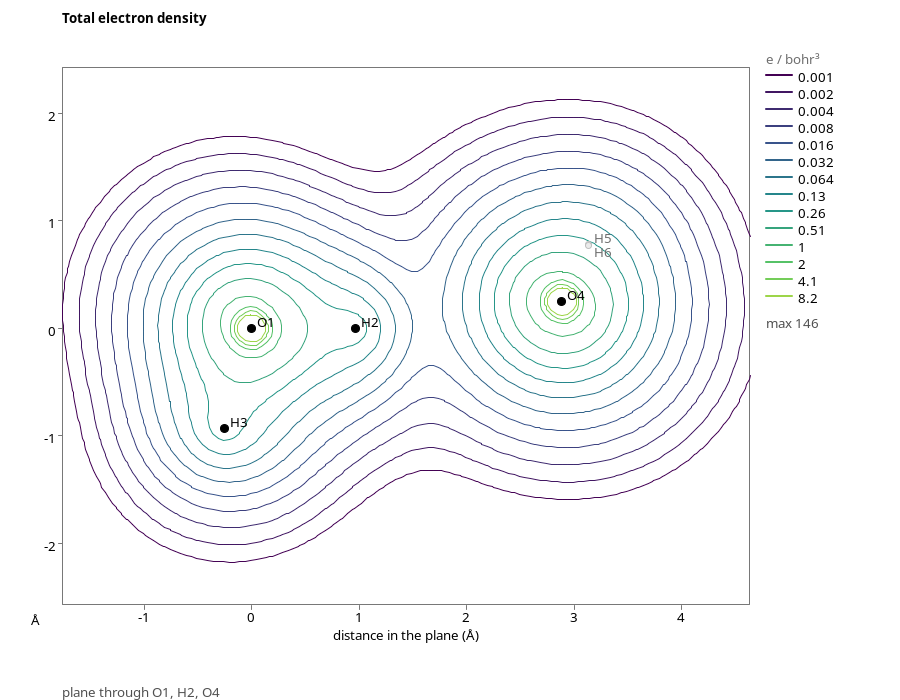
\includegraphics[width=0.8\linewidth]{hydrogen-bond/total-density.ecce-9.5.3-dev.png}
	\caption{Total electron density of the water dimer in the plane through O1, H2 and O4 (\menu{Density Map}). The contour levels double from 0.001~e/bohr$^3$ (0.001, 0.002, 0.004, \ldots), so each ring inward has twice the density of the one outside it. Only the outermost rings enclose both molecules.}
	\label{fig:hb-density}
\end{figure}

The \menu{Density Profile} along the line from O1 to O4, which passes almost through H2, puts numbers on the waist of the map (figure~\ref{fig:hb-profile}). The density is in electrons per cubic bohr (one bohr is \SI{0.529}{\angstrom}), on a logarithmic axis where each grid line is ten times the one below. Between H2 and O4 the density falls to a minimum of 0.0255~e/bohr$^3$, 0.66~\AA\ from H2. In the covalent O1--H2 bond it does not fall below 0.34~e/bohr$^3$, about thirteen times as much. The profile shows that the two molecules share very little electron density, because the hydrogen bond is mostly the electrostatic attraction of two separate molecules rather than an electron pair shared between them. Hence it is far weaker than a covalent bond, while the small density between H2 and O4 is still there, and the next view shows what kind of contact it is.
\index{Density Profile!hydrogen bond}

\begin{figure}[htbp]
	\centering
	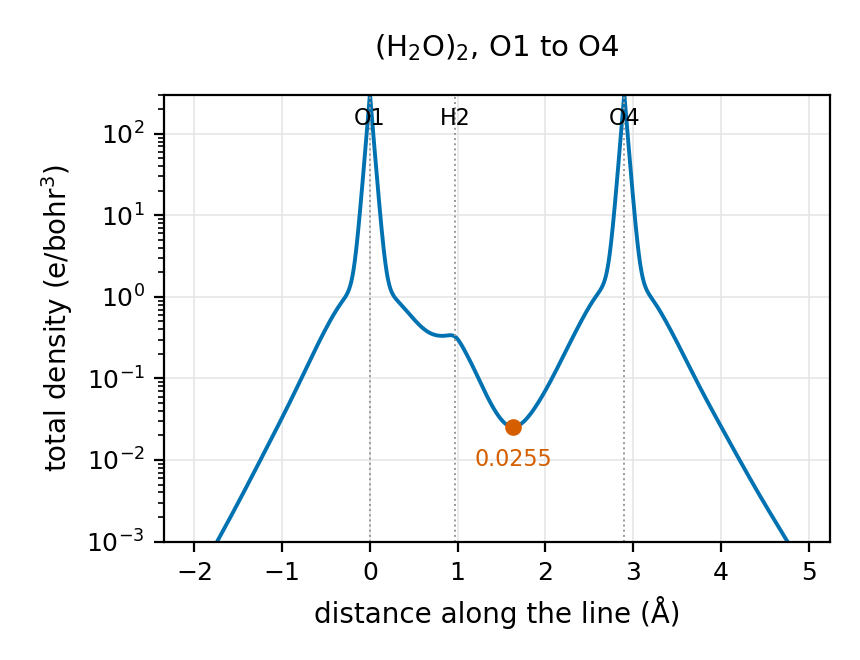
\includegraphics[width=0.6\linewidth]{hydrogen-bond/density-profiles.ecce-9.5.3-dev.png}
	\caption{Total electron density along the line from O1 to O4 of the water dimer (\menu{Density Profile}, logarithmic axis). The dot marks the lowest density between H2 and O4, 0.0255~e/bohr$^3$, about a thirteenth of the lowest density in the covalent O1--H2 bond.}
	\label{fig:hb-profile}
\end{figure}

\section{Non-covalent interactions}
The density map shows that there is a little density between H2 and O4, but not whether it pulls the molecules together or pushes them apart. The \menu{NCI} surface (non-covalent interactions) answers that, and it puts the hydrogen bond in one place in the picture (figure~\ref{fig:hb-nci}). ECCE draws the surface only where the electron density is low and changes slowly, which is true between molecules but not inside the covalent bonds or around the nuclei, so the bonds of each water molecule carry no surface and only the contacts between molecules do. It then colours the surface by the density there, with a sign that tells whether the density is gathered between two atoms or pushed apart: blue for attraction such as a hydrogen bond, green for weak contacts with little density, such as two molecules merely touching, and red for repulsion between atoms crowded too close. The colours run on one fixed scale for every calculation, so a blue surface in one molecule means the same as a blue surface in another.

In the water dimer the only surface is a small disc between H2 and O4, across the line between them, and it is blue. This shows that the density between the two molecules marks an attraction, because it is gathered between H2 and O4 rather than pushed apart. Hence the dotted line of the textbook has a place in the molecule, and the disc is where it crosses from one water molecule to the other.

\begin{figure}[htbp]
	\centering
	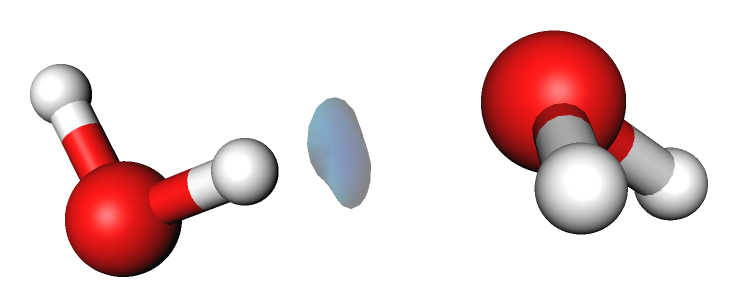
\includegraphics[width=0.6\linewidth]{hydrogen-bond/nci.ecce-9.5.3-dev.png}
	\caption{NCI surface of the water dimer (\menu{Properties > Orbitals > Surfaces}, \menu{NCI}), donor on the left and acceptor on the right. The only surface is the small disc between H2 and O4. Its colour tells the kind of contact on a fixed scale: blue attraction, as in a hydrogen bond; green a weak contact with little density; red repulsion. The disc is blue, an attraction; the surface is drawn partly transparent, which makes the blue look pale on a white background.}
	\label{fig:hb-nci}
\end{figure}

\section{In class}
Show the evidence in the order energy, distance, infrared, density: each is one more piece of evidence for the same bond, and the first three can be measured in a laboratory. The density map is the place to ask what the dotted line in the textbook stands for. It is not a line of electrons; the molecules stay separate, and what the map shows is a small extra amount of density between H and O on top of the overlap of two molecules. The NCI surface then puts the bond in one place, the blue disc between H2 and O4.

\section{History}
For a class, the origin of the idea shows that the hydrogen bond was proposed to explain the properties of water, the same properties the Background starts from. Latimer and Rodebush proposed in 1920 that a hydrogen atom held between two strongly electronegative atoms could bind them, to explain the properties of water and of hydrogen fluoride \cite{latimer1920}. Pauling made the hydrogen bond a part of structural chemistry in the 1930s, and it became central to biochemistry when it was shown to hold the base pairs of DNA and the helices and sheets of proteins together.
\index{Latimer, Wendell}\index{Rodebush, Worth}\index{Pauling, Linus}

\chapter{London dispersion}
\label{ch:t-dispersion}
\index{London dispersion}
\index{Argon dimer}
\index{Intermolecular interactions}
\eccexample{Examples > General Chemistry > Intermolecular interactions}

Two argon atoms carry no charge and no dipole, and their electron shells are closed, yet argon condenses when it is cold enough, so something must hold the atoms together. The attraction is London dispersion: the electron clouds of the two atoms fluctuate, and the fluctuations in one atom are correlated with those in the other, so that the pair is on average a little lower in energy close together than far apart. This chapter gives the teacher one curve, the energy of two argon atoms against their distance, to show a class that this attraction exists, how weak it is next to a hydrogen bond, and why it still matters. The argon dimer is the cleanest case to show, since nothing else contributes.

\section*{This requires}
Nothing beyond ECCE: the calculation is in the General Chemistry example set.

\section{The calculation}
The topic \menu{Intermolecular interactions} holds the argon dimer \emph{ar\_dimer}, optimised in ECCE in the same way as the water dimer of Chapter~\ref{sec:hydrogen-bond}. For the curve of figure~\ref{fig:disp-curve} the Ar--Ar distance was scanned (Chapter~\ref{ch:scans}), from \SI{0.4}{\angstrom} inside the optimised distance out to \SI{10}{\angstrom}. Each point is the energy of the pair relative to two argon atoms calculated separately, in kJ/mol, the energy per mole of pairs; a negative value means that the pair is held together by that much energy.

\section{The curve}
The curve shows how deep the attraction is and how it changes with distance. Its lowest point is at \SI{3.78}{\angstrom}, only \SI{1.2}{kJ.mol^{-1}} below two separate argon atoms (table~\ref{tab:disp-curve}). Spectroscopy of argon dimers in the gas phase puts the bottom of the real well at \SI{3.76}{\angstrom} and \SI{1.19}{kJ.mol^{-1}} (99.2~cm$^{-1}$) below the separate atoms \cite{herman1988}, so the calculated curve has both the position and the depth of the measured one. The two sides of the well are very different: moving the atoms \SI{0.4}{\angstrom} closer than the minimum raises the energy by \SI{1.3}{kJ.mol^{-1}}, more than the whole depth of the well, while moving them \SI{0.4}{\angstrom} apart costs only \SI{0.3}{kJ.mol^{-1}}. The steep inner wall is the repulsion of the two closed shells, which sets in abruptly once they touch, and the shallow outer side is the dispersion attraction, which dies away slowly with distance. Hence the curve shows both halves of the familiar picture of atoms as soft spheres, a hard core with a weak, long attractive tail. Beyond about \SI{8}{\angstrom} the points scatter by a few hundredths of a kJ/mol around zero; that is the numerical precision of the calculation, not a feature of the attraction.

\begin{figure}[htbp]
	\centering
	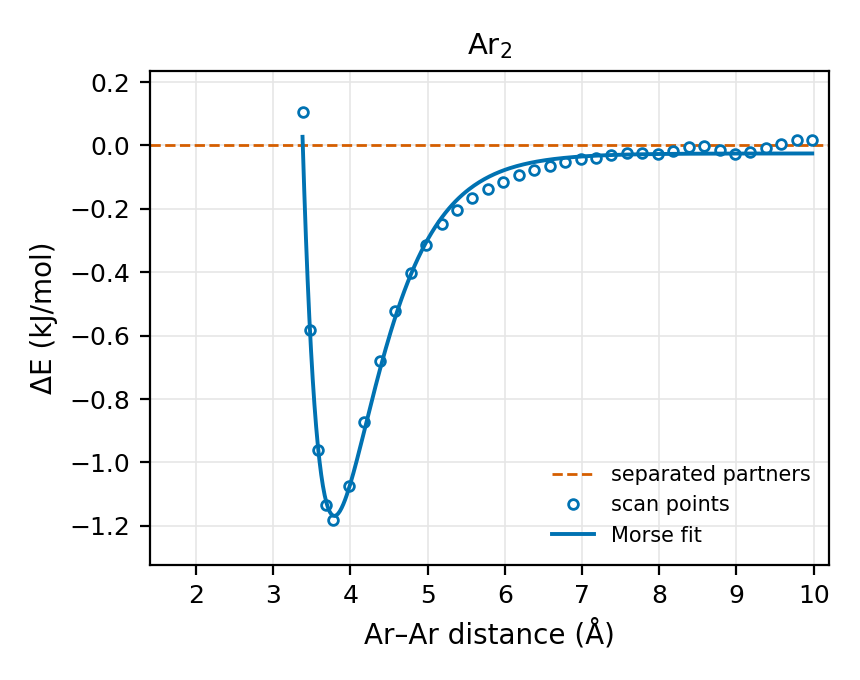
\includegraphics[width=0.6\linewidth]{dispersion/dispersion-curve.ecce-9.5.3-dev.png}
	\caption{Energy of the argon dimer against the Ar--Ar distance, from a relaxed scan in ECCE. Zero (dashed) is two argon atoms calculated separately. Note the energy scale, about twenty times smaller than that of the water dimer in figure~\ref{fig:hb-curve}.}
	\label{fig:disp-curve}
\end{figure}

\begin{table}[htbp]
	\centering
	\caption{The curve of figure~\ref{fig:disp-curve}. $\Delta E_\mathrm{min}$ is the lowest point, at the distance $R_\mathrm{min}$, and $\Delta E(R_\mathrm{max})$ the point at the largest distance $R_\mathrm{max}$, both relative to two separate argon atoms. Energies in kJ/mol.}
	\label{tab:disp-curve}
	\begin{tabular}{rrrr}
		\toprule
		$R_\mathrm{min}$ (\AA) & $\Delta E_\mathrm{min}$ & $\Delta E(R_\mathrm{max})$ & $R_\mathrm{max}$ (\AA) \\
		\midrule
		3.78 & $-1.2$ & 0.0 & 9.98 \\
		\bottomrule
	\end{tabular}
\end{table}

The comparison with the hydrogen bond puts the depth in proportion. The water dimer, scanned in the same way, is \SI{25.9}{kJ.mol^{-1}} deep (Chapter~\ref{sec:hydrogen-bond}), about twenty times deeper than the argon well. At room temperature $RT$, the typical energy that molecules exchange in collisions, is \SI{2.5}{kJ.mol^{-1}}, twice the depth of the argon well, so collisions break an argon pair apart almost as soon as it forms. Hence argon is a gas at room temperature and becomes a liquid only when it is cooled far enough for collisions to be gentle compared with the depth of the well. Argon boils at \SI{87.3}{K} (\SI{-185.9}{\celsius}) \cite{gosman1969}, where $RT$ is \SI{0.73}{kJ.mol^{-1}}, less than the depth of the well.
\index{Relaxed scan!interaction curves}

\section{Non-covalent interactions}
The \menu{NCI} surface (\menu{Properties > Orbitals > Surfaces}, \menu{NCI}), described with the water dimer in Chapter~\ref{sec:hydrogen-bond}, shows the contact between the two argon atoms in the same way. ECCE draws it only where the electron density is low and changes slowly, and colours it on one fixed scale: blue for an attraction with density gathered between two atoms, as in a hydrogen bond, green for a weak contact with very little density, and red for atoms crowded too close. In the argon dimer at its minimum the only surface is a single disc halfway between the two atoms, across the line joining them, and it is green (figure~\ref{fig:disp-nci}).

This figure shows that the two atoms meet in a contact with very little electron density, because green is the colour the fixed scale gives where the density between the atoms is close to zero. Hence we can see that the argon atoms are only touching, held by the weak attraction of the shallow well in figure~\ref{fig:disp-curve}, and not by an attraction with density gathered between them as in a hydrogen bond.
\index{NCI}

\begin{figure}[htbp]
	\centering
	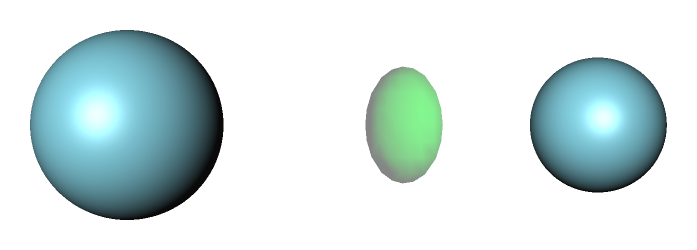
\includegraphics[width=0.6\linewidth]{dispersion/nci.ecce-9.5.3-dev.png}
	\caption{NCI surface of the argon dimer at its minimum (\menu{Properties > Orbitals > Surfaces}, \menu{NCI}). The only surface is the disc halfway between the two atoms. Its colour tells the kind of contact on a fixed scale: blue attraction, as in a hydrogen bond; green a weak contact with little density; red repulsion. The disc is green. The molecule is turned so that the disc shows; the left atom is nearer the viewer and looks larger.}
	\label{fig:disp-nci}
\end{figure}

\section{Three contacts side by side}
The NCI surfaces of three chapters set side by side (figure~\ref{fig:disp-nci-three}) give a class the kinds of contact in one picture: the argon dimer of this chapter, the water dimer of Chapter~\ref{sec:hydrogen-bond} and Na$^+\cdots$H$_2$O of Chapter~\ref{ch:t-ion-dipole}. Each has one disc between the partners. The argon disc is green, while the discs of the hydrogen bond and of the ion--water contact are both pale blue and look much alike, so the colour separates a weak dispersion contact from an attraction with density between the partners, but not a hydrogen bond from an ion--dipole contact; their strengths are told apart by the energies of the curves. None of the three shows red, since at the optimised distance no atoms are pushed together too closely.

This figure shows that dispersion is a different kind of contact from the hydrogen bond and the ion--dipole attraction, because the same fixed colour scale makes the argon disc green and the other two blue. Hence we can see in one picture that argon atoms are held by a weaker kind of contact than the one that holds two water molecules together or a water molecule to a dissolved ion.

\begin{figure}[htbp]
	\centering
	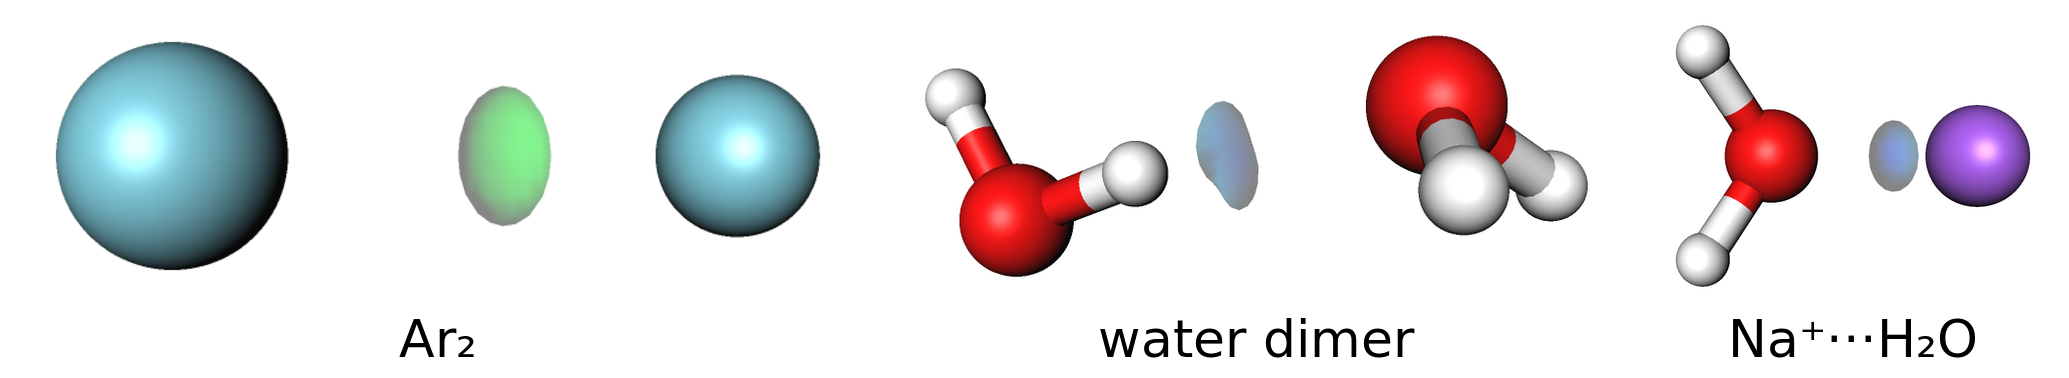
\includegraphics[width=\linewidth]{dispersion/nci-three.ecce-9.5.3-dev.png}
	\caption{NCI surfaces of the argon dimer (left, figure~\ref{fig:disp-nci}), the water dimer (middle, figure~\ref{fig:hb-nci}) and Na$^+\cdots$H$_2$O (right, figure~\ref{fig:id-nci}), each at its optimised structure, on the same fixed colour scale: blue attraction, green a weak contact with little density, red repulsion. The argon disc is green, the other two are blue; the surfaces are drawn partly transparent, which makes the blue look pale on a white background.}
	\label{fig:disp-nci-three}
\end{figure}

\section{In class}
Start with the question why argon, with no charges, no dipoles and full shells, becomes a liquid at all, and then show figure~\ref{fig:disp-curve} with its numbers next to those of the water dimer. Figure~\ref{fig:disp-nci-three} then shows the difference in colour: green for argon, blue for the hydrogen bond and for the ion next to a water molecule. The attraction between two single atoms is weak, but dispersion acts between every pair of atoms in contact, so it adds up for large molecules; this is why the boiling points of the straight-chain alkanes rise with chain length.

\section{History}
Van der Waals gave real gases an attraction between their molecules in his thesis of 1873, as the constant $a$ of his equation of state, without saying where the attraction came from \cite{vanderwaals1873}. Debye in 1920 and Keesom in 1921 traced it to the electric moments of the molecules: a permanent dipole or quadrupole induces a dipole in its neighbour (Debye), and permanent moments that rotate attract each other on average (Keesom) \cite{debye1920,keesom1921}. Neither mechanism applies to atoms of the noble gases, which have no permanent moments, and yet argon condenses. Jones (later Lennard-Jones) fitted an intermolecular potential with an attractive and a repulsive power of the distance to the equation of state of argon in 1924 \cite{jones1924}, and in 1931 settled on the form with $R^{-6}$ attraction and $R^{-12}$ repulsion that carries his name \cite{lennardjones1931}.
\index{van der Waals, Johannes Diderik}\index{Debye, Peter}\index{Keesom, Willem Hendrik}\index{Lennard-Jones, John}

The $R^{-6}$ attraction itself was explained by quantum mechanics. Eisenschitz and London calculated it for two hydrogen atoms in 1930, and London gave the general treatment the same year: the momentary dipoles of the two electron distributions are correlated, which lowers the energy of the pair by an amount that falls off as $R^{-6}$ \cite{eisenschitz1930,london1930}. London called the effect dispersion, after its connection with the optical dispersion of the atoms, and his 1937 paper in the Transactions of the Faraday Society gave the theory in English \cite{london1937}.
\index{London, Fritz}\index{Eisenschitz, Robert}

\chapter{Packing and unit cells}
\label{ch:t-packing}
\XXX[to be written: close packing, unit cells and coordination numbers in metals and salts]

\chapter{Molecular, covalent and layered solids}
\label{ch:t-solids}
\XXX[to be written: ice, dry ice, quartz, diamond and graphite compared]

\chapter{Bragg's law and X-ray diffraction}
\label{ch:t-bragg}
\XXX[to be written: a powder pattern from a crystal, and what the peaks mean]

\chapter{Photograph 51 and the alpha helix}
\label{ch:t-photograph-51}
\XXX[to be written: fibre diffraction patterns of DNA and a helical protein]

\chapter{Reaction energies and activation}
\label{ch:t-reaction-energies}
\XXX[to be written: an SN2 reaction: reaction energy, barrier and the Arrhenius equation]

\chapter{Acids and bases}
\label{ch:t-acids-bases}
\XXX[to be written: proton affinities and the site a proton prefers]

\chapter{Chemical equilibrium}
\label{ch:t-equilibrium}
\XXX[to be written: equilibrium constants from calculated free energies]

\chapter{Hartree-Fock and density functional theory}
\label{ch:t-hf-dft}
\XXX[to be written: what each method leaves out, shown on the same molecule]

\chapter{Basis sets}
\label{ch:t-basis-sets}
\XXX[to be written: how a property converges as the basis set grows]

\chapter{Restricted and unrestricted calculations}
\label{ch:t-restricted-unrestricted}
\XXX[to be written: closed and open shells, and spin contamination]



\appendix
\part{Appendices}
\chapter{Organizer menus and settings}
\label{ch:menus-organizer}
\checkedwith{9.5.3-dev}{e6ff4018a}
\index{Organizer!menus}
\index{Organizer!Preferences}

\helppage{organizer-menus}
\helppage{organizer-menubar}
\eccesource{src/apps/organizer data/client/config/ResourceDescriptor.xml src/wxgui/wxdialogs/GlobalPrefs.C}

This appendix goes through the Organizer menu by menu: the menu bar, the toolbar, the right-click menus of the tree and the project table, and the pages of the \menu{Preferences} window. Each entry says in a line or two what the item does, so that you can look up an item you have not used before without opening it. Keep in mind that several menus are rebuilt every time the selection changes, which means that what a menu offers, and which entries are grey, depends on what you have selected and, for a calculation, on its run state. Where that matters, the entry says so. Keyboard shortcuts are given where ECCE defines them.

\section{File}
\index{File menu}
The \menu{File} menu is rebuilt with every change of selection.
\begin{description}
	\item[\menu{New}] A submenu of what can be created in the nearest project or folder at or above the selection, or in the home folder when nothing is selected: a project, a calculation for each registered code, an MD study or a workflow. The entries are the same as those of \menu{New...} in the right-click menu.
	\index{File menu!New}
	\item[\menu{Upload File...}] Copies a file from this computer into the selected calculation; offered only when a calculation is selected.
	\index{File menu!Upload File...}
	\item[\menu{Download File...}] Saves the selected file to this computer; offered when a file, rather than a folder or a calculation, is selected.
	\index{File menu!Download File...}
	\item[\menu{New Structure...}] (\textsf{Ctrl+N}) Opens an empty Builder.
	\index{File menu!New Structure...}
	\item[\menu{Import Calculation from Output File...}] Makes a new calculation from the output file of a calculation that was run outside ECCE. It is offered whatever is selected.
	\index{File menu!Import Calculation from Output File...}\index{Importing an output file}
	\item[\menu{Import GROMACS Run...}] Makes a GROMACS study from the run directory of a simulation run outside ECCE.
	\index{File menu!Import GROMACS Run...}
	\item[\menu{Open Example Calculations}] Shows the example calculations that come with ECCE in the Organizer.
	\index{File menu!Open Example Calculations}
	\item[\menu{Export > Supporting Information...}] Writes the selected calculations, or all calculations below a selected folder, as one multi-structure XYZ file with the final geometry of each in \AA{}. The comment line of each structure holds the name, charge, multiplicity, total and Gibbs energies as stored, the code and the method. ECCE then asks whether to write a CSV or \LaTeX{} table of the same values beside the XYZ file, and, when some calculations are marked as excluded, whether to include them. The same files can be written from a terminal with \cmd{ecce-si-export}.
	\index{File menu!Export}\index{Supporting information}\index{ecce-si-export}
	\item[\menu{Quit}] (\textsf{Ctrl+Q}) Closes the Organizer and ends the session; it asks first when \menu{Ask for confirmation on exit} is set in Preferences.
	\index{File menu!Quit}
\end{description}

\section{Edit}
\index{Edit menu}
The first three items make a new calculation from the selected one. They are the same as the three items of \menu{New from This} in the right-click menu, under longer names.
\begin{description}
	\item[\menu{Duplicate for Rerun}] A copy of the calculation with the same structure and settings, reset and ready to launch (\menu{New from This > Rerun}).
	\index{Edit menu!Duplicate for Rerun}\index{Rerun}
	\item[\menu{Duplicate Setup with Last Geometry}] A copy that starts from the geometry the calculation ended on (\menu{Continue from Last Geometry}).
	\index{Edit menu!Duplicate Setup with Last Geometry}
	\item[\menu{Duplicate with Final Orbitals}] As the previous item, but the copy also starts from the final orbitals of the calculation (\menu{Continue from Final Orbitals}).
	\index{Edit menu!Duplicate with Final Orbitals}
	\item[\menu{Cut}] (\textsf{Ctrl+X}) Puts the selection on the Organizer's clipboard, so that \menu{Paste} moves it.
	\item[\menu{Copy}] (\textsf{Ctrl+C}) Puts the selection on the clipboard, so that \menu{Paste} copies it.
	\item[\menu{Paste}] (\textsf{Ctrl+V}) Moves or copies what is on the clipboard into the selected project or folder.
	\index{Edit menu!Cut}\index{Edit menu!Copy}\index{Edit menu!Paste}
	\item[\menu{Rename}] Renames the selected item; one item at a time.
	\item[\menu{Delete}] (\textsf{Del}) Deletes the selection, asking first when \menu{Confirm Deletes} is on. Backspace does the same in the tree.
	\index{Edit menu!Rename}\index{Edit menu!Delete}
	\item[\menu{Annotation...}] Opens an editor for the annotation of the selected item, which is a free-text note kept with it.
	\index{Edit menu!Annotation...}\index{Annotation}
	\item[\menu{Find...}] (\textsf{Ctrl+F}) Opens the Find window, which lists the items below the folder given in \menu{From} whose name, or path from that folder, contains the text you type. Note that the search distinguishes upper and lower case. \ctrl{Open} selects the chosen result in the tree.
	\index{Edit menu!Find...}
	\item[\menu{Change Access Control...}] Sets who may read or change a project on a data server. It is grey for a local folder, which has only one user, and when more than one item is selected.
	\index{Edit menu!Change Access Control...}\index{Access control}
	\item[\menu{Preferences...}] Opens the \menu{ECCE Preferences} window (Section~\ref{sec:org-prefs}).
	\index{Edit menu!Preferences...}
\end{description}

\section{Options}
\index{Options menu}
The check items of this menu are kept between sessions; those marked (on) are on by default.
\begin{description}
	\item[\menu{Show Toolbar}] (on) Shows or hides the toolbar.
	\item[\menu{Show Run State Legend}] (on) Shows or hides the legend of the run-state icons.
	\item[\menu{Show Lines in Tree View}] (on) Draws the lines that join the items of the tree.
	\item[\menu{Show Run States in Tree}] (on) Shows the run-state icon of each calculation in the tree.
	\item[\menu{Show ECCE Internal Files}] Shows the files that ECCE keeps inside a calculation for its own use.
	\index{Options menu!Show Toolbar}\index{Options menu!Show Run State Legend}\index{Options menu!Show Lines in Tree View}\index{Options menu!Show Run States in Tree}\index{Options menu!Show ECCE Internal Files}
	\item[\menu{Set Home as Root}] Makes your home folder the top of the tree, which is rebuilt when you switch this.
	\item[\menu{Ask for File Name at Creation}] (on) Asks for a name when you create a project, a calculation or another item; when it is off, the item is named after its type. A workflow step is named in its own dialog either way.
	\item[\menu{Invoke Default Tool at Creation}] Opens the default tool of a new item as soon as it is created.
	\item[\menu{Confirm Deletes}] (on) Asks before \menu{Delete} removes anything.
	\item[\menu{Confirm Resets}] (on) Asks before an editor resets a task for a rerun, since the reset removes the output of the previous run.
	\index{Options menu!Set Home as Root}\index{Options menu!Ask for File Name at Creation}\index{Options menu!Invoke Default Tool at Creation}\index{Options menu!Confirm Deletes}\index{Options menu!Confirm Resets}
	\item[\menu{Sort Tree by}] Orders the tree by \menu{Type}, \menu{Name} or \menu{Date}, each also in reverse.
	\index{Options menu!Sort Tree by}
	\item[\menu{Project View}] Chooses the columns of the project table: \menu{Basic Properties}, \menu{Setup Properties}, \menu{Launch Properties} or \menu{All Properties}.
	\index{Options menu!Project View}\index{Project table!columns}
\end{description}

\section{Go}
\index{Go menu}
The \menu{Go} menu moves the selection through the tree in the way a file manager or a web browser does.
\begin{description}
	\item[\menu{Home}] (\textsf{Alt+Home}) Selects your home folder on the current server.
	\item[\menu{Up}] (\textsf{Alt+Up}) Selects the folder above the selection; grey at the top of the tree.
	\item[\menu{Back}] (\textsf{Alt+Left}) Returns to the place selected before.
	\item[\menu{Forward}] (\textsf{Alt+Right}) Goes forward again after \menu{Back}.
	\item[History list] Below a separator, the last 15 places selected, newest first, with the current one ticked; choosing one selects it.
	\index{Go menu!Home}\index{Go menu!Up}\index{Go menu!Back}\index{Go menu!Forward}\index{Go menu!history}
\end{description}

\section{Bookmarks}
\index{Bookmarks menu}
\begin{description}
	\item[\menu{Add to Bookmarks}] (\textsf{Ctrl+D}) Bookmarks the selected item.
	\item[\menu{Manage Bookmarks...}] Opens the Bookmark Editor, where you edit the name and the address of a bookmark, and where \ctrl{Add}, \ctrl{Delete}, \ctrl{Move Up} and \ctrl{Move Down} change the list.
	\item[Bookmark list] Below a separator, one entry per bookmark; choosing one selects that item in the tree.
	\index{Bookmarks menu!Add to Bookmarks}\index{Bookmarks menu!Manage Bookmarks...}\index{Bookmark Editor}
\end{description}

\section{Run Mgmt}
\index{Run Mgmt menu}
The \menu{Run Mgmt} menu acts on the selected calculation, and since what can be done with a job depends on how far it has come, its entries follow the run state. The states given below are those registered for the quantum-chemistry codes. With several calculations selected, the menu holds only \menu{Launch Selected...}, \menu{Reconnect Selected...}, \menu{Terminate Selected...} and \menu{Re-Parse Outputs}, and with anything other than calculations selected it is grey. The entries are listed in the order of the menu.
\begin{description}
	\item[\menu{Tail -f on Output File...}] (\textsf{Alt+L}) Opens a terminal that follows the output file as the job writes it; for running or waiting jobs.
	\item[\menu{Shell in Calculation Run Directory...}] (\textsf{Alt+S}) Opens a terminal in the run directory on the compute machine, from submission on.
	\item[\menu{Terminate Calculation...}] Stops the job on the compute machine; for submitted, running or waiting jobs.
	\item[\menu{Check Job Monitoring}] Reports whether the job monitor of the calculation is still running; for submitted, running or waiting jobs.
	\item[\menu{Check Job on Machine}] Asks the compute machine, over ECCE's own login, whether the process or queue job is still there and when the output was last written. Note that it only reports: the state is still set by the job monitor or by a reconnect.
	\item[\menu{Reconnect Job Monitoring}] Starts a new job monitor for a job started earlier. When the job cannot be reconnected the item is grey, and its help text gives the reason.
	\item[\menu{Force State to Failed}] Sets the state of a submitted, running or waiting job to failed without touching the job itself.
	\index{Run Mgmt menu!Tail -f on Output File...}\index{Run Mgmt menu!Shell in Calculation Run Directory...}\index{Run Mgmt menu!Terminate Calculation...}\index{Run Mgmt menu!Check Job Monitoring}\index{Run Mgmt menu!Check Job on Machine}\index{Run Mgmt menu!Reconnect Job Monitoring}\index{Run Mgmt menu!Force State to Failed}
	\item[\menu{Reset to Rerun}] (\textsf{Alt+R}) Resets a finished calculation so that it can be launched again, which removes the outputs of the previous run. Imported calculations are skipped with a message, because the reset would delete the only copy of their results.
	\item[\menu{Reset for Restart}] Sets the state back to ready and clears the reviewed mark, while the outputs stay.
	\item[\menu{Reset State}] A submenu that changes the state alone: \menu{Reset to completed}, \menu{Reset to incomplete}, \menu{Reset to imported} and \menu{Reset to killed}, each offered only from the other states.
	\item[\menu{Mark as Reviewed}] Marks the calculation as reviewed and records the date.
	\item[\menu{Mark as Unreviewed}] Removes the reviewed mark and its date.
	\index{Run Mgmt menu!Reset to Rerun}\index{Run Mgmt menu!Reset for Restart}\index{Run Mgmt menu!Reset State}\index{Run Mgmt menu!Mark as Reviewed}\index{Run Mgmt menu!Mark as Unreviewed}
	\item[\menu{Cleanup Run Directory Files}] Removes the files of the calculation from its run directory on the compute machine; for finished, killed or failed calculations.
	\item[\menu{View Run Log...}] Shows the log that ECCE kept of the launch and the monitoring of the job.
	\item[\menu{View Input file...}] (\textsf{Alt+I}) Opens the input file in the editor set in Preferences.
	\item[\menu{View Output File...}] (\textsf{Alt+O}) Opens the output file in that editor; for finished, imported, killed or failed calculations.
	\index{Run Mgmt menu!Cleanup Run Directory Files}\index{Run Mgmt menu!View Run Log...}\index{Run Mgmt menu!View Input file...}\index{Run Mgmt menu!View Output File...}
	\item[\menu{Launch Selected...}] Launches the selected calculations; offered for a calculation that is created or ready.
	\item[\menu{Reconnect Selected...}] Reconnects the job monitoring of the selection; grey when no selected job can be reconnected.
	\item[\menu{Terminate Selected...}] Stops the jobs of the selected calculations; only with several selected.
	\item[\menu{Re-Parse Outputs}] Runs the parsers again over the outputs stored with a finished calculation.
	\index{Run Mgmt menu!Launch Selected...}\index{Run Mgmt menu!Reconnect Selected...}\index{Run Mgmt menu!Terminate Selected...}\index{Run Mgmt menu!Re-Parse Outputs}
\end{description}

\section{Tools}
\index{Tools menu}
The \menu{Tools} menu has two parts. The upper part is the same whatever is selected, while the lower part lists the tools of the selected item under the grey heading \menu{For \textit{name}:}. With two calculations selected only the upper part is shown, and with more than two the menu is grey.
\begin{description}
	\item[\menu{Register Machines...}] Opens the Machine Registration window, where a compute machine is defined.
	\item[\menu{Machine Browser...}] Opens the Machine Browser, which shows the registered machines.
	\item[\menu{Allocations...}] Lists each cluster account of your machine profiles and how much of it is used, read in the background over logins that are already open.
	\index{Tools menu!Register Machines...}\index{Tools menu!Machine Browser...}\index{Tools menu!Allocations...}
	\item[\menu{Periodic Table...}] (\textsf{Ctrl+P}) Opens the periodic table.
	\item[\menu{Energy Calculator...}] Opens the Energy Calculator, which gives the energy difference between sums of calculations, such as the two sides of a reaction.
	\item[\menu{New Calculations in Another Code...}] Makes one new calculation in another code from each selected calculation, with a setup that you make once for all of them.
	\index{Tools menu!Periodic Table...}\index{Tools menu!Energy Calculator...}\index{Tools menu!New Calculations in Another Code...}
	\item[\menu{Batch Add from SMILES...}] Makes one calculation per row of a table of names, SMILES strings and measured values, from a template calculation in the folder.
	\item[\menu{QSAR Table...}] Builds the descriptor table of the selected folder or calculations from the descriptor groups ticked in a list: counts, topological indices, property models, Gasteiger charges, surface areas, and the HOMO, LUMO, gap, dipole and charges of the calculations.
	\item[\menu{QSAR Analysis...}] A principal component analysis of the descriptor table of the selected folder, and a PLS regression against a measured column, with the report and the plots.
	\index{Tools menu!Batch Add from SMILES...}\index{Tools menu!QSAR Table...}\index{Tools menu!QSAR Analysis...}\index{QSAR}
	\item[\menu{Builder}] Shown instead of the lower part when the selection has no tools of its own; opens an empty Builder, as \menu{File > New Structure...} does.
	\item[\menu{Electronic Structure Editor...}] (\textsf{Ctrl+E}) Opens the Calculation Editor of the selected calculation.
	\item[\menu{Builder...}] (\textsf{Ctrl+B}) Opens the structure of the selected calculation in the Builder.
	\item[\menu{Basis Set Tool...}] (\textsf{Ctrl+S}) Opens the Basis Set Tool for the selected calculation.
	\item[\menu{Launcher...}] (\textsf{Ctrl+L}) Opens the Launcher of the selected calculation, from the ready state on.
	\item[\menu{Viewer...}] (\textsf{Ctrl+R}) Opens the results of the selected calculation in the viewer.
	\item[MD editors] For an MD task, the editor of its kind: \menu{\textit{code} MD Prepare Editor...}, or the Optimize, Energy or Dynamics editor (\textsf{Ctrl+E}), named after the code of the task, NWChem or GROMACS.
	\index{Tools menu!Electronic Structure Editor...}\index{Tools menu!Builder...}\index{Tools menu!Basis Set Tool...}\index{Tools menu!Launcher...}\index{Tools menu!Viewer...}\index{Tools menu!MD editors}
\end{description}
Which tools a code offers, and in which run states, is registered for each code in \cmd{ResourceDescriptor.xml}. For a quantum-chemistry calculation, all of the tools above except the Launcher are offered in every state.

\section{Help}
\index{Help menu}
\begin{description}
	\item[\menu{ECCE Help}] (\textsf{Ctrl+H}) Opens ECCE's help in the web browser set in Preferences.
	\item[\menu{Running Codes on This Computer}] Opens the help page on running the computational codes on this computer.
	\item[\menu{Report a Problem...}] Collects what is needed to find out what went wrong into a folder \cmd{ecce-bug-\textit{date}} in your home folder, and packs it as a zip archive beside it. On Linux and macOS the archive holds the ECCE version, a description of the system, the logs of the services and the results of ECCE's diagnostic checks; on Windows it holds the ECCE version, the Windows version, the ECCE logs and the last ECCE crash records of the Windows event log. ECCE sends nothing itself, so you attach the archive to your report.
	\item[\menu{How to Cite ECCE...}] Opens the help page on citing ECCE.
	\item[\menu{About ECCE...}] Shows the version of ECCE and, for a development build, its commit.
	\index{Help menu!ECCE Help}\index{Help menu!Running Codes on This Computer}\index{Help menu!Report a Problem...}\index{Help menu!How to Cite ECCE...}\index{Help menu!About ECCE...}\index{Reporting a problem}
\end{description}

\section{Developer}
\index{Developer menu}
The \menu{Developer} menu is there only when the environment variable \cmd{ECCE\_DEVELOPER} is set.
\begin{description}
	\item[\menu{Generate Theory/RunType Test Suite}] Makes a project \cmd{\textit{name}\_TestSuite} beside the selected calculation, with one calculation for each combination of theory and run type of its code.
	\item[\menu{View Properties...}] Shows the stored properties (metadata) of the selected item.
	\item[\menu{Manage Data Servers...}] Opens the list of data servers; the tree is rebuilt when the list is closed. For everyday use, \menu{Preferences > Data} and the \menu{Servers} button on the toolbar do the same job.
	\index{Developer menu!Generate Theory/RunType Test Suite}\index{Developer menu!View Properties...}\index{Developer menu!Manage Data Servers...}
\end{description}

\section{Toolbar}
\index{Organizer!toolbar}
From left to right, named by the tooltip of each button:
\begin{description}
	\item[\menu{Go to user home on current server}, \menu{Go up}, \menu{Go back}, \menu{Go forward}] As \menu{Home}, \menu{Up}, \menu{Back} and \menu{Forward} in the \menu{Go} menu.
	\item[\menu{Cut}, \menu{Copy}, \menu{Paste}, \menu{Rename}, \menu{Delete}] As in the \menu{Edit} menu.
	\item[\menu{Search File...}] As \menu{Edit > Find...}.
	\item[\menu{Refresh}] Reads the selected part of the tree again from where it is stored.
	\item[\menu{Upload File...}, \menu{Download File...}] As in the \menu{File} menu.
	\item[\menu{View Properties...}] As \menu{Developer > View Properties...}, but on the toolbar it is there without \cmd{ECCE\_DEVELOPER} too.
	\item[\menu{Servers}] A menu of the remembered SSH folders and ECCE servers, each ticked while connected; ticking an entry connects to it and clearing the tick disconnects. Below them, \menu{Add Server...} remembers another location and \menu{Manage Servers...} opens \menu{Preferences > Data}. Note that the central server configured for the session is not listed.
	\index{Organizer!toolbar!Servers}\index{Servers menu}
\end{description}

\section{Right-click menus}
\index{Organizer!right-click menu}\index{Context menu|see{Organizer, right-click menu}}
Right-clicking an item in the tree, or rows of the project table, opens a menu that is built from the selection, so that most entries below appear only for the kind of item they apply to.
\begin{description}
	\item[\menu{New...}] As \menu{File > New} for the nearest project or folder, and below a separator \menu{Import Calculation from Output File...}; grey where nothing can be created.
	\item[\menu{Cut}, \menu{Copy}, \menu{Paste}] As in the \menu{Edit} menu; \menu{Paste} is grey while the clipboard is empty.
	\item[\menu{Move to...}, \menu{Copy to...}] Open a list of the folders of every tree the Organizer shows, servers included, and move or copy the selection into the one you choose.
	\item[\menu{Rename}, \menu{Delete}] As in the \menu{Edit} menu. For a system folder these and \menu{Cut} are grey.
	\index{Organizer!right-click menu!Move to...}\index{Organizer!right-click menu!Copy to...}
	\item[\menu{Duplicate for Rerun}] On a task of an MD study: a copy of the task that keeps its place in the study.
	\item[\menu{New from This}] On a calculation: \menu{Rerun}, \menu{Continue from Last Geometry} and \menu{Continue from Final Orbitals}, the three \menu{Duplicate} items of the \menu{Edit} menu. The last is grey, with the reason as its help text, when the code or the stored results cannot provide a starting guess. In the project table the submenu also holds \menu{In Another Code...}, the same as \menu{Tools > New Calculations in Another Code...}. For a periodic calculation, \menu{Screen Sites with MLP...} makes one MLP calculation for each interstitial site or vacancy pair of the host.
	\index{Organizer!right-click menu!New from This}\index{Screen Sites with MLP}
	\item[\menu{Make Workflow...}] On a calculation: moves it into a new workflow as its first step; grey, with the reason, when it cannot be moved.
	\item[\menu{Move into Workflow}] On a calculation: a submenu of the workflows in the same folder, which moves the calculation into the one chosen.
	\item[\menu{Run}] On a calculation: \menu{Launch...}, \menu{Reconnect...}, \menu{Terminate}, \menu{Re-Parse Outputs} and \menu{Shell in Run Directory}, each grey when it does not fit the run state. With calculations selected in the project table instead: \menu{Launch Selected...}, \menu{Reconnect Selected...}, \menu{Terminate Selected...} and \menu{Re-Parse Outputs}.
	\index{Organizer!right-click menu!Make Workflow...}\index{Organizer!right-click menu!Move into Workflow}\index{Organizer!right-click menu!Run}
	\item[\menu{Make Workflow from Selected...}, \menu{Move Selected into Workflow}] With two or more calculations selected in the project table: move them into a new workflow, with links between them, or into a workflow of the folder.
	\item[\menu{Compare Energies...}] With two or more calculations selected in the project table, or with a folder selected: the energies of those calculations relative to each other.
	\item[\menu{Site Screening Results}] In the folder of a site screen, which holds a calculation named \cmd{host}: $E - E(\mathrm{host})$ of the finished site calculations, as an ensemble that can be shown in the Builder.
	\item[\menu{Terminate Calculation...}, \menu{Shell in Calculation Run Directory...}] On a task of an MD study, in the states where they apply.
	\index{Organizer!right-click menu!Compare Energies...}\index{Compare Energies}\index{Organizer!right-click menu!Site Screening Results}
\end{description}
\index{Organizer!server tree}
The root of a remembered server's tree has a right-click menu of its own, with \menu{Connect} or \menu{Disconnect}, and \menu{Remove from list}. \menu{Disconnect} closes the Organizer's logins to the server and folds its tree, while \menu{Remove from list} forgets the entry without deleting anything on the server.

\section{Preferences}
\label{sec:org-prefs}
\index{Preferences}
\menu{Edit > Preferences...} opens the \menu{ECCE Preferences} window. Each change is saved as you make it, so there is nothing to confirm: \ctrl{Close} hides the window, and \ctrl{Reset All} returns every setting to its default. The settings apply to all ECCE applications, not only to the Organizer.

\subsection*{General}
\index{Preferences!General}
\begin{description}
	\item[\menu{Font Size}] \menu{Small}, \menu{Medium}, \menu{Large} or \menu{Extra Large}.
	\item[\menu{Use the system font size}] Uses the font size of the desktop instead of ECCE's 10\,pt; takes effect when the applications are next started.
	\item[\menu{Date Format}, \menu{Time Format}] How dates and times are written in ECCE's windows.
	\item[\menu{Units}] The units in which energies, lengths and angles are shown: \menu{AU} (hartree, bohr, radian), \menu{CGS} (kcal\,mol\textsuperscript{$-1$}, \AA, degree) or \menu{SI} (kJ\,mol\textsuperscript{$-1$}, nm, radian).
	\item[\menu{Beep on errors}, \menu{Beep on warnings}] Sound the bell with an error or a warning message.
	\item[\menu{Focus follows mouse over input fields}] An input field takes the keyboard while the pointer is over it.
	\item[\menu{Ask for confirmation on exit}] Asks before the session ends.
	\item[\menu{Close remote shells on exit}] Closes the terminals opened on compute machines when the session ends.
	\item[\menu{Save data and compute server passwords between sessions}] Keeps the passwords, so that you are not asked for them at the next start.
	\item[\menu{Check for new releases}] At most once a day, asks GitHub which releases exist, sending only ECCE's version; nothing is downloaded or installed. The setting is locked when \cmd{ECCE\_NO\_UPDATE\_CHECK} is set or when the administrator of the installation has switched the check off.
	\item[\menu{Also tell me about previews (alpha and beta releases)}] Includes preview releases in the check.
	\item[\menu{Quick transparency}] Draws transparent orbitals and isosurfaces faster, but less accurately where lobes overlap; takes effect the next time one is shown in the Builder.
	\item[\menu{Show the MO diagram for ECCE-QM calculations}] Offers the MO diagram for ECCE-QM calculations; for the other codes it is always offered. It takes effect the next time a calculation is opened in the Builder, and it is grey when the administrator has switched the MO diagram off.
	\index{Preferences!Units}\index{Preferences!Check for new releases}\index{Preferences!Quick transparency}\index{Preferences!MO diagram}
\end{description}

\subsection*{Colours}
\index{Preferences!Colours}
\begin{description}
	\item[\menu{Colour scheme}] \menu{Jmol} or \menu{ECCE (classic)}, the element colours of the 3-D viewer, the periodic table and the thumbnails. An open Builder changes at once, and other windows when they are next opened.
	\item[\menu{Style}] \menu{Flat} or \menu{Shaded} run-state icons in the Organizer tree and its legend.
	\index{Preferences!element colours}\index{Preferences!run-state icons}
\end{description}

\subsection*{External programs}
\index{Preferences!External programs}
Each row offers a list of presets and \menu{Other}, which takes a command with its arguments.
\begin{description}
	\item[\menu{Editor}] The editor for input and output files. \menu{Default} uses \cmd{VISUAL} or \cmd{EDITOR} when either is set, and otherwise \cmd{vi} (\cmd{open -t} on macOS). Terminal editors run in the terminal set in the next row.
	\item[\menu{Terminal}] The terminal for terminal editors and for the shells that the Organizer, the Launcher and MD Prepare open, locally or on a compute machine. \menu{Default} is \cmd{xterm} on Linux and Terminal on macOS.
	\item[\menu{Web browser}] The browser for Help. \menu{Automatic} uses \cmd{xdg-open}, \cmd{x-www-browser} or \cmd{sensible-browser}, whichever is found first.
\end{description}
When \cmd{ECCE\_EDITOR}, \cmd{ECCE\_TERMINAL} or \cmd{ECCE\_BROWSER} is set, it overrides the setting, and the page says so.

\subsection*{Data}
\index{Preferences!Data}
\begin{description}
	\item[\menu{Folder}] Where the calculations on this computer are kept. \ctrl{Change...} picks another folder, and \ctrl{Open} shows the folder in the file manager.
	\item[\menu{Servers}] The list of remembered servers, with \menu{Name}, \menu{Type} and \menu{Address}. \ctrl{Add Server...} and \ctrl{Edit...} open the server dialog, whose \menu{Connect at start} decides whether the Organizer connects when it starts, and \ctrl{Remove} takes a server out of the list without deleting anything on it.
	\item[\menu{Discard the programs' own binary files once results.h5 is written}] Applies to jobs that finish after it is set, and at present to Gaussian 16 checkpoint files only; \menu{Continue from Final Orbitals} then reads the orbitals from \cmd{results.h5}.
	\index{Preferences!Servers}\index{results.h5}
\end{description}

\subsection*{Advanced}
\index{Preferences!Advanced}
This page holds switches for testing and troubleshooting. Each of them sets an environment variable for the ECCE applications; when the variable is already set in the environment, that value wins, and the page says so.
\begin{description}
	\item[\menu{OpenGL drawing}] \menu{Automatic}, \menu{Software-safe} or \menu{Hardware}. \menu{Automatic} decides from the OpenGL renderer that the 3-D view runs on (\cmd{ECCE\_GL\_PATH}).
	\item[\menu{Native (C++) Details dialogs}] Opens the theory Details dialogs with the C++ engine instead of the Python one.
	\item[\menu{Per-pixel lighting off}] Draws the 3-D view with fixed-function lighting, for when the picture is wrong or blank.
	\item[\menu{No progress records for older calculations}] The Organizer does not work out a progress record for a calculation that has none.
	\item[\menu{3-D view diagnostics}] Writes the lighting path and the OpenGL visual to the error output.
	\item[\menu{Window and panel diagnostics}] Writes how windows are raised and panels placed to the error output.
	\item[\menu{MO-diagram symmetry log}] Appends the symmetry analysis behind the MO diagram to the file given (by default \cmd{mosym.log}).
	\item[\menu{Data-server login log}] Appends what happens during data-server logins to the file given (by default \cmd{davauth.log}).
	\item[\menu{Remembered ssh logins}] The hosts whose SSH passwords are kept by \menu{Remember on this computer}; \ctrl{Forget} removes one. The row is shown only where a password store is available.
	\index{Preferences!OpenGL drawing}\index{Preferences!Remembered ssh logins}
\end{description}

\subsection*{Gateway window}
\index{Preferences!Gateway window}
This page is present only when the Gateway window is in use, that is, when ECCE is started with \cmd{ECCE\_GATEWAY\_WINDOW=1}.
\begin{description}
	\item[\menu{Show system busy icon}] (on) The ECCE icon of the Gateway window moves while work is going on.
	\item[\menu{Always on top}] Keeps the Gateway window above other windows, although the window manager may override this.
	\item[\menu{Left click invokes new tool}] Swaps what a click on a tool button does: bring up the copy of the tool that is already open, or start a new one.
	\item[\menu{Horizontal Orientation}, \menu{Vertical Orientation}] The tool buttons of the Gateway window in a row or in a column.
\end{description}

\chapter{Builder and viewer menus and settings}
\label{ch:menus-builder}
\index{Builder!menus}
\index{Viewer!menus}
\index{Builder!Preferences}
\index{Properties list}

\helppage{viewer-panels}
\eccesource{src/apps/builder src/wxviz data/client/config/PropertyPanelDescriptor.xml}
\XXX[ chapter to be written]

\section{Background}

\section{What ECCE shows}

\section{Procedure}

\section{Results}


\chapter{Settings files and environment variables}
\label{ch:settings}
\index{Preferences}
\index{Environment variables}
\index{Settings files}


\eccesource{src/util/Preferences.C src/util/Ecce.C bin docs/AGENTS.md}
\XXX[ chapter to be written]

\section{Background}

\section{What ECCE shows}

\section{Procedure}

\section{Results}

\section{Coupling with other codes}
% What feeds this calculation (a cheaper screen, a structure from another code)
% and what it feeds (refinement, a property from the code best at it); which
% steps a workflow or recipe automates and which are a manual hand-off.




\backmatter

\printbibliography[heading=bibintoc, title={Bibliography}]

\cleardoublepage
\phantomsection
\addcontentsline{toc}{chapter}{Index}
\printindex

\end{document}
